% -- DÚVIDAS --
% -> No início de cada capítulo, seção ou subseção não há \par. Pq?
% Figura não sendo inserida na posição delimitada pelo código - Figura 17
% Necessita-se de parágrafos em todos os trechos de texto?
% Como centralizar verticalmente apenas uma célula em tabelas?
% Conversão de Tabelas http://www.tablesgenerator.com/latex_tables
% Manual ABNTeX2 http://mirror.unl.edu/ctan/macros/latex/contrib/abntex2/doc/abntex2.pdf
% Corrigir tab_2
% Dúvidas marcadas com um [?]
% Links autoref estão bugados, levando p/ a legenda da imagem ao invés da imagem
% Apendice sem identação correta e sem justificação
% Como referenciar capítulo?
% Adicionar \url{} nos links da bibliografia
% Escrever conclusão
% ----- Após revisão
% Alterar imagens com fundo transparente (Ex.: Figura 05)
% Corrigir notas de rodapé
% Alterar tamanho das imagens
%[?] COLOCAR LIVROS QUE UTILIZAMOS PARA APRENDER PADORES DE PROJETO?
% Verificar se falta alguma referencia
% Rever imagens, adicionar circulos, sublinhados, etc, necessários!


\documentclass[
% -- opções da classe memoir --
12pt,				% tamanho da fonte
openright,			% capítulos começam em pág ímpar (insere página vazia caso preciso)
oneside,			% para impressão em verso e anverso. Oposto a oneside
a4paper,			% tamanho do papel. 
% -- opções da classe abntex2 --
%chapter=TITLE,		% títulos de capítulos convertidos em letras maiúsculas
%section=TITLE,		% títulos de seções convertidos em letras maiúsculas
%subsection=TITLE,	% títulos de subseções convertidos em letras maiúsculas
%subsubsection=TITLE,% títulos de subsubseções convertidos em letras maiúsculas
% -- opções do pacote babel --
%english,			% idioma adicional para hifenização
%french,				% idioma adicional para hifenização
%spanish,			% idioma adicional para hifenização
brazil,				% o último idioma é o principal do documento
]{abntex2}


% ---
% PACOTES
% ---

% ---
% Pacotes fundamentais 
% ---
\usepackage{cmap}				% Mapear caracteres especiais no PDF
\usepackage{lmodern}			% Usa a fonte Latin Modern			
\usepackage[T1]{fontenc}		% Selecao de codigos de fonte.
\usepackage[utf8]{inputenc}		% Codificacao do documento (conversão automática dos acentos)
\usepackage{lastpage}			% Usado pela Ficha catalográfica
\usepackage{indentfirst}		% Indenta o primeiro parágrafo de cada seção.
\usepackage{color}				% Controle das cores
\usepackage{graphicx}			% Inclusão de gráficos
\usepackage{amsmath}
\usepackage{epstopdf}
\usepackage{float}
\usepackage{hyperref}
\usepackage{multirow}
\usepackage{ragged2e}
\usepackage{caption}
% ---

% ---
% Pacotes adicionais, usados apenas no âmbito do Modelo Canônico do abnteX2
% ---
\usepackage{lipsum}				% para geração de dummy text
\usepackage{mathtools}
% ---

% ---
% Pacotes de citações
% ---
\usepackage[brazilian,hyperpageref]{backref}	 % Paginas com as citações na bibl
\usepackage[alf]{abntex2cite}	% Citações padrão ABNT

% --- 
% CONFIGURAÇÕES DE PACOTES
% --- 

% ---
% Configurações do pacote backref
% Usado sem a opção hyperpageref de backref
\renewcommand{\backrefpagesname}{Citado na(s) página(s):~}
% Texto padrão antes do número das páginas
\renewcommand{\backref}{}
% Define os textos da citação
\renewcommand*{\backrefalt}[4]{
	\ifcase #1 %
	Nenhuma citação no texto.%
	\or
	Citado na página #2.%
	\else
	Citado #1 vezes nas páginas #2.%
	\fi}%
% ---




% ---
% Informações de dados para CAPA e FOLHA DE ROSTO
% ---
\titulo{Redes Veiculares: Tendências e Estudo de Caso}
\autor{ARTHUR ALBUQUERQUE ZOPELLARO SOARES\\
		LAURO DE LACERDA CAETANO}
\local{Campos dos Goytacazes}
\data{2016}
\orientador{MSc. VINÍCIUS BARCELOS} % [?] Verificar com o orientador
\instituicao{%
	Instituto Federal Fluminense -- IFF
	\par
	Campus Campos Centro
	\par
	Sistemas de Informação}
\tipotrabalho{Trabalho de Conclusão de Curso}
% O preambulo deve conter o tipo do trabalho, o objetivo, 
% o nome da instituição e a área de concentração 
\preambulo{Trabalho de conclusão de curso apresentado ao Instituto
	Federal de Educação, Ciência e Tecnologia Fluminense como requisito
	parcial para conclusão do curso de Bacharelado em Sistemas de Informação.}
% ---


% ---
% Configurações de aparência do PDF final

% alterando o aspecto da cor azul
\definecolor{blue}{RGB}{41,5,195}

% informações do PDF
\makeatletter
\hypersetup{
	%pagebackref=true,
	pdftitle={\@title}, 
	pdfauthor={\@author},
	pdfsubject={\imprimirpreambulo},
	pdfcreator={LaTeX with abnTeX2},
	pdfkeywords={abnt}{latex}{abntex}{abntex2}{trabalho acadêmico}, 
	colorlinks=true,       		% false: boxed links; true: colored links
	linkcolor=blue,          	% color of internal links
	citecolor=blue,        		% color of links to bibliography
	filecolor=magenta,      		% color of file links
	urlcolor=blue,
	bookmarksdepth=4
}
\makeatother
% --- 

% --- 
% Espaçamentos entre linhas e parágrafos 
% --- 

% O tamanho do parágrafo é dado por:
\setlength{\parindent}{1.3cm}

% Controle do espaçamento entre um parágrafo e outro:
\setlength{\parskip}{0.2cm}  % tente também \onelineskip

% ---
% compila o indice
% ---
\makeindex
% ---

% ----
% Início do documento
% ----
\begin{document}
	
	% Retira espaço extra obsoleto entre as frases.
	\frenchspacing 
	
	% ----------------------------------------------------------
	% ELEMENTOS PRÉ-TEXTUAIS
	% ----------------------------------------------------------
	% \pretextual
	
	% ---
	% Capa
	% ---
	\imprimircapa
	% ---
	
	% ---
	% Folha de rosto
	% (o * indica que haverá a ficha bibliográfica)
	% ---
	\imprimirfolhaderosto*
	% ---
	
	% ---
	% Inserir a ficha bibliografica
	% ---
	
	% Isto é um exemplo de Ficha Catalográfica, ou ``Dados internacionais de
	% catalogação-na-publicação''. Você pode utilizar este modelo como referência. 
	% Porém, provavelmente a biblioteca da sua universidade lhe fornecerá um PDF
	% com a ficha catalográfica definitiva após a defesa do trabalho. Quando estiver
	% com o documento, salve-o como PDF no diretório do seu projeto e substitua todo
	% o conteúdo de implementação deste arquivo pelo comando abaixo:
	%
	% \begin{fichacatalografica}
	%     \includepdf{fig_ficha_catalografica.pdf}
	% \end{fichacatalografica}
	\begin{fichacatalografica}
		\vspace*{\fill}					% Posição vertical
		\hrule							% Linha horizontal
		\begin{center}					% Minipage Centralizado
			\begin{minipage}[c]{12.5cm}		% Largura
				
				\imprimirautor
				
				\hspace{0.5cm} \imprimirtitulo  / \imprimirautor. --
				\imprimirlocal, \imprimirdata-
				
				\hspace{0.5cm} \pageref{LastPage} p. : il. (algumas color.) ; 30 cm.\\
				
				\hspace{0.5cm} \imprimirorientadorRotulo~\imprimirorientador\\
				
				\hspace{0.5cm}
				\parbox[t]{\textwidth}{\imprimirtipotrabalho~--~\imprimirinstituicao,
					\imprimirdata.}\\
				
				\hspace{0.5cm}
				1. Redes Veiculares.
				2. WAVE.
				3. VEINS.
				I. MSc. Vinícius Barcelos.
				II. Instituto Federal Fluminense.
				III. Campus Campos Centro.
				IV. Título\\ 			
				
				\hspace{8.75cm} CDU 02:141:005.7\\
				
			\end{minipage}
		\end{center}
		\hrule
	\end{fichacatalografica}
	% ---
	
	% ---
	% Inserir errata
	% ---
	% Comentar este preambulo caso não exista errata.
	
	%\begin{errata}
	%Elemento opcional da \citeonline[4.2.1.2]{NBR14724:2011}. Exemplo:
	%
	%\vspace{\onelineskip}
	%
	%FERRIGNO, C. R. A. \textbf{Tratamento de neoplasias ósseas apendiculares com
	%reimplantação de enxerto ósseo autólogo autoclavado associado ao plasma
	%rico em plaquetas}: estudo crítico na cirurgia de preservação de membro em
	%cães. 2011. 128 f. Tese (Livre-Docência) - Faculdade de Medicina Veterinária e
	%Zootecnia, Universidade de São Paulo, São Paulo, 2011.
	%
	%\begin{table}[htb]
	%\center
	%\footnotesize
	%\begin{tabular}{|p{1.4cm}|p{1cm}|p{3cm}|p{3cm}|}
	%  \hline
	%   \textbf{Folha} & \textbf{Linha}  & \textbf{Onde se lê}  & \textbf{Leia-se}  \\
	%    \hline
	%    1 & 10 & auto-conclavo & autoconclavo\\
	%   \hline
	%\end{tabular}
	%\end{table}
	%
	%\end{errata}
	% ---
	
	% ---
	% Inserir folha de aprovação
	% ---
	
	% Isto é um exemplo de Folha de aprovação, elemento obrigatório da NBR
	% 14724/2011 (seção 4.2.1.3). Você pode utilizar este modelo até a aprovação
	% do trabalho. Após isso, substitua todo o conteúdo deste arquivo por uma
	% imagem da página assinada pela banca com o comando abaixo:
	%
	% \includepdf{folhadeaprovacao_final.pdf}
	%
	\begin{folhadeaprovacao}
		
		\begin{center}
			{\ABNTEXchapterfont\large\imprimirautor}
			
			\vspace*{\fill}\vspace*{\fill}
			{\ABNTEXchapterfont\bfseries\Large\imprimirtitulo}
			\vspace*{\fill}
			
			\hspace{.45\textwidth}
			\begin{minipage}{.5\textwidth}
				\imprimirpreambulo
			\end{minipage}%
			\vspace*{\fill}
		\end{center}
		
		Trabalho aprovado. \imprimirlocal, %DATA:\\
		\vspace*{\fill}
		
		%O nome do orientador é inserido automaticamente
		\centering
		\rule{10cm}{.3mm}\\
		\textbf{\imprimirorientador\\INSTITUTO FEDERAL FLUMINENSE - IFF\\} Orientador
		\vspace*{\fill}
		
		\rule{10cm}{.3mm}\\
		\textbf{ D.Sc. \\INSTITUTO FEDERAL FLUMINENSE - IFF}
		\vspace*{\fill}
		
		\rule{10cm}{.3mm}\\
		\textbf{ M.Sc. BANCA 2\\INSTITUTO FEDERAL FLUMINENSE - IFF}
		\vspace*{\fill}
		
		\rule{10cm}{.3mm}\\
		\textbf{ M.Sc. BANCA 2\\INSTITUTO FEDERAL FLUMINENSE - IFF}
		\vspace*{\fill}
		
		\begin{center}
			\vspace*{0.5cm}
			{\large\imprimirlocal}
			\par
			{\large\imprimirdata}
			\vspace*{1cm}
		\end{center}
		
	\end{folhadeaprovacao}
	% ---
	
	% ---
	% Dedicatória
	% ---
	\begin{dedicatoria}
		\vspace*{\fill}
		\centering
		\noindent
		\textit{A nossos pais, mestres e amigos
			} \vspace*{\fill}
	\end{dedicatoria}
	% ---
	
	% ---
	% Agradecimentos
	% ---
	\begin{agradecimentos} % Agradecimentos do Lauro

		\par Minha gratidão a meu Deus por ter me dado este tema em um momento de angústia particular e ter me ensinado em Provérbios 3:13-14 que adquirir conhecimento é uma bênção.

		\par Agradeço aos meus pais pelo amor e motivação doados. Com carinho, meu obrigado aos amigos mais chegados pela força concedida durante a jornada deste trabalho.

		\par O meu agradecimento especial a todos os mestres, servidores e colegas de profissão do Instituto Federal Fluminense, com quem tanto aprendi e dividi dúvidas, incertezas, alegrias e desesperos nestes anos de curso. 

		\par Um notável agradecimento ao CNPq que, durante o período deste curso, me concedeu uma bolsa de intercâmbio no exterior, transformando-me em um estudante mais completo. 

		\par Obrigado a você também, leitor, pela apreciação deste trabalho monográfico. Espero que, de alguma forma, ele faça alguma diferença para as suas pesquisas.

		\begin{flushright}
			\textit{Lauro de Lacerda Caetano}
		\end{flushright}
		
	\end{agradecimentos} 

	\begin{agradecimentos} % Agradecimentos do Arthur

		\par Agradeço aos meus parentes pela base familiar provida durante todos estes anos, permitindo meu crescimento pessoal e acadêmico. Muito obrigado também ao apoio dos amigos nesta difícil jornada de conclusão de curso.

		\par Devo agradecer aos professores pelo suporte e conhecimento transmitido, sendo parte essencial, não só para conclusão do trabalho, mas como também durante toda a faculdade. Um agradecimento especial ao nosso Orientador Vinícius Barcelos pela paciência, clarividência e por nos mostrar os melhores caminhos a serem seguidos.

		\par E um agradecimento especial ao meu amigo Lauro de Lacerda pela confiança no meu trabalho e por me apresentar o potencial de Redes Veiculares. 

		\begin{flushright}
			\textit{Arthur Albuquerque Zopellaro Soares}
		\end{flushright}

	\end{agradecimentos}

	% ---

	% ---
	% Epígrafe
	% ---
	\newpage
	\begin{epigrafe}
		\vspace*{\fill}
		\begin{flushright}
			\textit{"Nothing is too wonderful to be true,\\
				 if it be consistent with the laws of nature."\\
				(Michael Faraday)}
		\end{flushright}
	\end{epigrafe}
	% ---
	
	% ---
	% RESUMOS
	% ---
% resumo em português
\setlength{\absparsep}{18pt} % ajusta o espaçamento dos parágrafos do resumo
\begin{resumo}

	\par Este trabalho descreve o desenvolvimento da tecnologia de redes veiculares, sua padronização e suas ferramentas. Em especial, a norma IEEE 1609 é investigada em maior detalhe. São citados diversos exemplos de aplicações possíveis para a tecnologia veicular. Encontram-se analisados diversos softwares de simulação que, quando integrados, permitem que simulações de veículos se conectem em rede. A tecnologia é simulada e analisada em um estudo de caso criado em cenário na cidade do Rio de Janeiro. Tutoriais de instalação e de criação de novos cenários de simulação estão adicionados neste trabalho.

	\vspace{\onelineskip}
			
	\textbf{Palavras-chaves}: Redes Veiculares, WAVE, VEINS
\end{resumo}
	
% resumo em inglês
\begin{resumo}[Abstract]
	\begin{otherlanguage*}{english}
		
		\par This work describes the development of the vehicular networking technology, its standardization and tools. Specifically, the IEEE 1609 standard is investigated in detail. Several examples of vehicular technology applications are given. A group of  simulation tools is analyzed and compared. When some of them are integrated, they allow vehicles to be connected in networks. The technology is simulated and scrutinized on a case study in a scenario in Rio de Janeiro city. Installation and implementation guides that help creating new scenarios are attached to this work.			
	 
		\vspace{\onelineskip}
		
		\noindent 
		\textbf{Key-words}: Vehicular Networks, WAVE, VEINS
		
	\end{otherlanguage*}
\end{resumo}
		
	% ---
	% inserir lista de ilustrações
	% ---
	\pdfbookmark[0]{\listfigurename}{lof}
	\listoffigures*
	\cleardoublepage
	% ---
	
	% ---
	% inserir lista de tabelas
	% ---
	\pdfbookmark[0]{\listtablename}{lot}
	\listoftables*
	\cleardoublepage
	% ---
	
	% ---
	% inserir lista de abreviaturas e siglas
	% ---
	\begin{siglas}
		\item[ANATEL] Agência Nacional de Telecomunicações
		\item[ASN.1] Abstract Syntax Notation One
		\item[BSM] Basic Safety Message
		\item[BSS] Basic Service Set
		\item[BSSID] BSS Identification
		\item[CCH] Control Channel
		\item[DNS] Domain Name System
		\item[DS] Distribution System
		\item[DSRC] Dedicated Short Range Communications
		\item[EDCA] Enhanced Distributed Channel Access
		\item[ETSI] European Telecommunications Standards Institute
		\item[FCS] Frame Check Sequence
		\item[FTP] File Transfer Protocol
		\item[GPS] Global Positioning System
		\item[HTTP] HyperText Transfer Protocol
		\item[IEEE] Institute of Electrical and Electronics Engineers
		\item[IBSS] Independent BSS 
		\item[IoV] Internet of Vehicles
		\item[ITS] Intelligent Transportation Systems 
		\item[LAN] Local Area Network
		\item[LLC] Logical Link Control
		\item[MAC] Media Access Control
		\item[MANET] Mobile Ad Hoc Network
		\item[MIMO] Multiple Input Multiple Output
		\item[MLME] MAC subLayer Management Entity
		\item[MLMEX] MAC subLayer Management Entity Extension
		\item[NED] Network Description
		\item[OFDM] Orthogonal Frequency Division Multiplexing
		\item[OSI] Open Systems Interconnection 
		\item[OCB] On the Context of BSS
		\item[OBU] On Board Unit
		\item[PHY] Physical Layer
		\item[PLME] Physical Layer Management Entity
		\item[PSC] Provider Service Context 
		\item[PSID] Provider Service Identifier
		\item[RSA] Roadside Alert
		\item[RSU] Roadside Unit 	
		\item[SAE] Society of Automotive Engineers
		\item[SCH] Service Channel 
		\item[SDEE] Secure Data Exchange Entity
		\item[SSME] Security Services Management Entity
		\item[SUMO] Simulator of Urban Mobility
		\item[TCP] Transfer Control Protocol
		\item[TraCI] Traffic Command Interface 
		\item[TPID] Transport Protocol Identification
		\item[UTC] Universal Time Coordinated
		\item[V2I] Vehicle-to-Infrastructure 
		\item[V2V] Vehicle-to-Vehicle 
		\item[VANET] Vehicle Ad Hoc Network 
		\item[VEINS] Vehicles in Network Simulation 
		\item[WAN] Wide Area Network
		\item[WAVE] Wireless Access in Vehicular Enviroments
		\item[WME] WAVE Management Entity 
		\item[WRA] WAVE Routing Advertisement 
		\item[WSA] WAVE Service Advertisement
		\item[WSM] WAVE Short Message
		\item[WSMP] WAVE Short Message Protocol
		\item[WSMP-N] WSMP Network 
		\item[WSMP-T] WSMP Transport
		
		
	\end{siglas}
	% ---
	
	% ---
	% inserir o sumario
	% ---
	\pdfbookmark[0]{\contentsname}{toc}
	\tableofcontents*
	\cleardoublepage
	% ---
	
	
	
	
	% ----------------------------------------------------------
	% ELEMENTOS TEXTUAIS
	% ----------------------------------------------------------
	\textual
	
	% ----------------------------------------------------------
	% Introdução
	% ----------------------------------------------------------
	\chapter[Introdução]{Introdução}
%	\addcontentsline{toc}{chapter}{Introdução}

	%\justify
	
	\par Com objetivo de promover integração mundial e contribuir para o crescimento da economia, cooperando no deslocamento de pessoas e mercadorias, os meios de transporte são objetos fundamentais na atual sociedade. Estes determinam aquilo que é chamado de “compressão do tempo e do espaço”, onde as distâncias do mundo se encurtam, ou seja, podem ser mais facilmente percorridas, reduzindo gastos e tempo de trajeto (Harvey, 1989).
	
	\par Aliados aos meios de transporte, os sistemas de comunicação cooperam para o aumento da segurança e da comodidade nos percursos. Em ambiente marítimo, itens como rádios auxiliam na conversação entre embarcações e bases marítimas. Transponders e sonares ajudam na transmissão de coordenadas e no descobrimento de embarcações próximas. 
	
	\par Nos transportes aéreos, o mesmo transponder passou a ser utilizado na aviação comercial, tornando-se item obrigatório. Este coopera para a comunicação de aviões com torres de comando além de ser parte importante dos sistemas anticolisão. Através da troca de informação entre estes sistemas, é possível que aviões projetem informações de outras aeronaves em um raio considerável, como localização, rumo, altitude e velocidade.
	
	\par Os transportes terrestres, contudo, não evoluíram na mesma velocidade em que os veículos marítimos e aéreos no que diz respeito aos sistemas de comunicação. Dadas as claras \textbf{externalidades}{\footnote{efeitos sociais, econômicos e ambientais indiretamente causados pela venda de um produto ou serviço}} negativas causadas pelos veículos nas cidades como trânsito, poluição e acidentes, vê-se como necessário o pronto desenvolvimento de ferramentas de comunicação que auxiliem na mitigação destas externalidades.

	\par Dotados de maior conscientização sobre os fatos, os governos têm examinado o papel do veículo na cadeia de valor da indústria automobilística, buscando tratar as externalidades citadas. Além disso, a comunidade científica tem trabalhado no desenvolvimento de mecanismos que visam melhorar a qualidade de vida dos seres humanos em ambiente veicular. 
	
	\par A Internet dos Veículos apresenta-se como um conceito que expande o grau de ubiquidade da tecnologia da informação para o meio veicular. Como tecnologia, a internet dos veículos tem por objetivo a aplicação de recursos para solução ou mitigação de problemas, além servir de ferramenta para a geração de novos conhecimentos. E como tecnologia da informação, esta permite o tratamento e a difusão de dados. Portanto, a eventual consolidação deste conceito no mercado possibilitaria o surgimento de um novo paradigma de Internet, abrindo um amplo horizonte para a ciência com o surgimento de novas ferramentas de comunicação, entretenimento e segurança.
	
	\par Vista como subclasse da Internet das Coisas, a Internet dos Veículos é uma rede que também integra dispositivos incorporados de sensores (veículos, itens de sinalização, unidades de acostamento), software e rede de dados, possibilitando que veículos e mais objetos coletem e troquem informações. A partir do processamento das informações, os veículos podem tornar-se mais inteligentes, sendo capazes de auxiliar na tomada de decisões até de maneira parcial ou totalmente autônomas, visando a segurança e bem estar dos passageiros e pedestres.
	
	\par As redes de comunicação veiculares, parte fundamental para incremento da inteligência no meio veicular, continuam em plena evolução. O estudo do funcionamento destas tem mais de uma década, sendo iniciado pelas VANETs (\textit{Vehicular Ad Hoc NETworks} ou Redes Ad Hoc Veiculares), passando por diversos protocolos de teste, até chegar ao estabelecimento de famílias de padrões. Duas destas se destacam, a primeira família chamada de Acesso sem fio em Ambientes Veiculares (WAVE) contém um conjunto de padrões criados pelo Instituto de Engenheiros Elétricos e Eletrônicos(IEEE) que foram submetidos a diversas baterias de testes e provas de conceito. Na Europa, a família de padrões para Sistemas de Transportes Inteligentes do Instituto de Padrões de Telecomunicações Europeu(ETSI) se iguala em notoriedade na comunidade científica.
	
	\par Segundo expectativas de mercado, 75\% dos carros do mundo estarão conectados em 2020, e o crescimento da Internet dos Veículos trará em torno de US\$2,94 bilhões em receitas{\footnote{http://press.trendforce.com/node/view/1880.html (acesso em 13 de maio 2016)}}. Com um amplo apoio do Departamento de Transporte dos Estados Unidos, a comunicação entre veículos está perto de se tornar obrigatória para automóveis em circulação neste país{\footnote{https://www.transportation.gov/fastlane/dialogue-industry-conversation-between-cars(acesso em 14 de maio 2016)}}. Na Europa, a implantação da comunicação veicular também está acelerada. Foi criado um consórcio chamado Car2Car a partir da iniciativa de fabricantes de veículos europeus. Este consórcio sem fins lucrativos tem por objetivo aumentar a eficiência e segurança no tráfego rodoviário a partir da utilização de redes veículares.
	
	\par As redes veiculares apresentam-se como área promissora para a ciência e para o mercado de trabalho. É possível que nos próximos anos apareçam \textit{startups} focadas no desenvolvimento de aplicações voltadas para entretenimento e segurança veicular. Além disso, empresas de tecnologia 3G e 4G podem se aproveitar de uma ampliação do alcance das comunicações interveiculares para oferecer planos de dados, transformando os veículos numa extensão da atual Internet. Ademais, com o advento dos veículos autônomos servindo-se da imprescindível existência de redes de comunicação, podemos visionar o aumento da segurança dos transportes e do bem estar de condutores  e passageiros.
	
	
	\section{Justificativa}
	
	\par O atual mercado conta com diversas ferramentas para irradiação de informações no trânsito. Assim como painéis digitais em vias de alta densidade veicular cooperam para melhor fluidez do trânsito, redes sociais como o Waze alertam eventuais acidentes no caminho de condutores. 
	
	\par Entretanto, foi percebido que os atuais meios de comunicação de tráfego rodoviário ainda são limitados no que diz respeito à propagação rápida de mensagens de emergência no trânsito. Isto ocorre pois a maioria das ferramentas dependem do processamento de seus servidores antes da entrega da informação.
	
	\par As Redes Veiculares, por usarem comunicação ponto-a-ponto, propagam a informação com menor atraso e por isso podem ser usadas para enviar informações de situações em tempo real a motoristas, ajudando na tomada de decisão dos condutores e prevenindo possíveis acidentes.
	
	\par Equipes de resgate são constantemente acionadas para o socorro de pessoas e necessitam de tráfego livre no trajeto até o socorrido. Quando há trânsito no perímetro urbano ou em rodovias, as equipes de resgate têm seu trabalho atrapalhado por obstruções na passagem. Mesmo com giroscópio e sirene emitindo sinais visual e sonoro, o atraso no atendimento pode ser gerado por um efeito estocástico de obstruções. Como consequência do atraso até o local de atendimento, a demora para socorro de vítimas pode ser fatal.
	
	\par Há, portanto, que se testar a utilização de métodos mais eficientes de propagação de mensagens utilizando-se de Redes Veiculares. Antes de entrar em produção, é preciso utilizar métodos de avaliação em caráter de simulação a fim de testar a transmissão destas mensagens de emergência entre unidades de acostamento e veículos. Seria possível antecipar situações de prováveis obstruções enviando mensagens aos carros das redondezas, acelerando a liberação de vias para um resgate com menor atraso. 	
	
	\section{Objetivos}
	
	\par Neste trabalho pretende-se desenvolver um estudo de caso em ambiente de simulação de tráfego urbano empregando redes veiculares para a propagação em broadcast de mensagens oriundas de veículos de segurança pública. 
	
	\par Também é objetivo contribuir com uma ampla revisão bibliográfica para análise da família padrões IEEE 1609, especialmente as normas já homologadas pelo IEEE. Estes padrões formarão uma consistente base teórica para o estudo de caso.
	
	\par Além disso, este trabalho tem finalidade de orientar por meio de tutoriais:
	
	\begin{itemize}
		\item a instalação de um conjunto de softwares para a simulação de redes veiculares;
		\item a criação de novos cenários e experimentos de simulação utilizando esta tecnologia.
	\end{itemize}
	
	\section{Metodologia}
	
	\par Como base teória para um estudo de caso, serão discorridos conceitos de redes de computadores e de redes veiculares, que foram padronizados pelo IEEE e outras organizações por meio das normas IEEE 802.11p, IEEE 1609 WAVE e SAE J2735. 
	
	\par Serão analisados simuladores de tráfego urbano e simuladores de redes a fim de encontrar um grupo que melhor trabalhe com simulações de redes veiculares. 
	
	\par Após definição deste grupo, será desenvolvido um estudo de caso em redes veiculares analisando os efeitos de uma aplicação, criada pelos autores deste trabalho, que transmite mensagens de emergência no trânsito. 

	\par Como fruto do desenvolvimento do estudo de caso serão criados tutoriais para facilitar a instalação e a criação de novos estudos que investiguem as redes veiculares.
	
	\newpage
	
	% ----------------------------------------------------------
	% PARTE - Fundamentação Teórica
	% ----------------------------------------------------------
	\chapter{Introdução à Redes sem fio} % verificar com o orientador
	
	\par Este capítulo apresenta as bases teóricas no estudo de redes de comunicação, seus principais padrões e características. Também serão estabelecidos conceitos iniciais de comunicação sem fio e suas normas, que servirão de base para um melhor entendimento dos padrões de redes veiculares que serão posteriormente discutidos neste trabalho.
		
	\section{Modelos de Referência}
	
	\par O estudo de redes de comunicação inicia no entendimento das duas mais relevantes arquiteturas de rede, os modelos de referência OSI e TCP/IP. 

	\subsection{Modelo OSI}
	
	\par No começo dos anos 80, diversas empresas perceberam que deveriam sair do modelo proprietário dos sistemas de rede para resolver problemas de incompatibilidade e falta de comunicação. O modelo de referência OSI foi o primeiro modelo criado para redes de comunicação e teve, à época, o objetivo de ajudar estas organizações a criar redes que pudessem ser compatíveis e interoperáveis umas com as outras.
	
	\par O modelo OSI foi liberado em 1984 contendo um conjunto de padrões que garantiram maior compatibilidade e operabilidade entre os vários tipos de tecnologias de rede produzidos por empresas ao redor do mundo. Apesar de outros modelos terem existido, o modelo de referência OSI é considerado a melhor ferramenta disponível para o envio e recebimento de dados em uma rede.
	
	\par O Modelo OSI foi dividido em 7 níveis que se inter-relacionam. Foi feito desta maneira para facilitar o entendimento de como a informação viaja através de uma rede. Cada nível ilustra uma função particular da rede. Uma camada conta com a próxima camada inferior para realizar funções mais primitivas e ocultar os detalhes destas funções. Para exemplificar, o modelo OSI descreve como os dados trafegam de uma aplicação através de um meio de rede até uma aplicação localizada em outro computador, mesmo que o emissor e o receptor estejam utilizando meios de rede diferentes. A \autoref{fig_1} apresenta a estrutura do modelo, composto de sete camadas ordenadas.
	
	% INSERIR FIGURA Modelo OSI
	\begin{figure} [H]
		\centering
		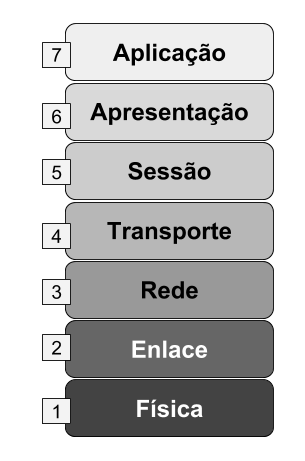
\includegraphics[scale=.5]{figuras/cap2/01ModeloOSI}
		\caption{\label{fig_1}Modelo OSI}
	\end{figure}
		
	\par Cada camada OSI contém um conjunto de funções executadas por programas para fazer os dados viajarem de uma origem até o destino de uma rede.
	
	\par A camada de aplicação é a mais próxima do usuário e provê serviços de rede para as aplicações. Esta, diferente dos outros níveis do modelo, não oferece serviços para outras camadas OSI superiores. Entretanto, realiza ajustes em procedimentos de recuperação de erros e no controle da integridade dos dados.
	
	\par A camada de apresentação garante que os dados da camada de aplicação de um sistema são legíveis pela camada de aplicação de outro sistema. Se necessário, a camada de apresentação traduz e estrutura múltiplos formatos de dados, usando um formato comum.
	
	\par Além de reportar problemas das camadas superiores, a camada de sessão fornece a estrutura de controle para comunicação entre as aplicações. Esta camada estabelece, gerencia e termina as conexões entre as aplicações.
	
	\par A camada de transporte segmenta os dados do sistema emissor e reúne os dados em um fluxo único no sistema recipiente. Isto possibilita a transferência de dados confiável e transparente entre as extremidades, oferecendo recuperação de erro e controle de fluxo de ponta a ponta. 
	
	\par A camada de rede oferece conectividade e seleção de caminho entre dois sistemas que podem estar em redes separadas geograficamente. Nela há o roteamento de pacotes e é a responsável por estabelecer, manter e terminar as conexões.
	
	\par A camada de enlace define como os dados são formatados para transmissão e como o acesso à rede é controlado. Envia \textit{frames} para sincronismo, controle de erro e controle de fluxo, se necessário. 
	
	\par A camada física define as especificações elétricas, mecânicas, procedurais e funcionais para ativação, manutenção e desativação de uma conexão física entre sistemas. A transmissão dos dados é binária. Características como níveis de voltagem, sincronismo das variações de tensão, taxas de dados físicos, distâncias máximas de transmissão, conectores físicos e outros atributos similares são definidos nas especificações da camada física.
	
	%-------
	
	\subsection{Modelo TCP/IP}
	
	\par Embora o modelo de referência OSI seja reconhecido mundialmente, há um outro padrão que tem uma visão histórica e sobremaneira técnica da Internet: a pilha de protocolos TCP/IP.
	
	\par A pilha de protocolos TCP/IP tem quatro camadas: Aplicação, Transporte, Internet e Acesso à Rede. Apesar de algumas camadas do modelo TCP/IP serem homônimas de algumas do modelo OSI, estas têm diferentes funções em cada modelo. A \autoref{fig_2} compara as camadas do modelo OSI e TCP/IP.
	
	% INSERIR IMAGEM Modelo OSI e TCP/IP	
	\begin{figure} [H]
		\centering
		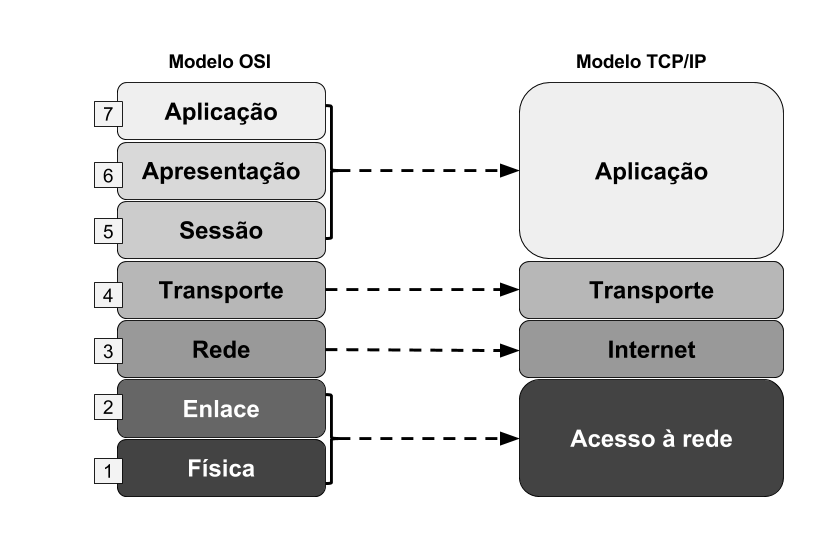
\includegraphics[scale=.5]{figuras/cap2/02ModeloOSIeTCP}
		\caption{\label{fig_2}Modelo OSI e TCP/IP}
	\end{figure}
	
	\par A camada de aplicação controla protocolos de alto nível, incluindo questões de representação, codificação e controle de diálogo. O modelo TCP/IP combina todas as questões relacionadas às aplicações em um único nível e garante que esses dados sejam devidamente empacotados para o próximo nível. Há diversos protocolos de aplicação, como FTP e o HTTP.
	
	\par A camada de transporte lida com questões de Qualidade de Serviço (\textit{Quality of Service} ou QoS) como confiabilidade, controle de fluxo e correção de erros. Um de seus protocolos é o TCP (\textit{Transmission Control Protocol} ou Protocolo de Controle de Transmissão), que oferece comunicações de rede confiáveis. 
	
	\par A camada de Internet tem a responsabilidade de enviar pacotes através de redes. Para interligação dessas redes, é necessário que o envio de dados a partir de uma rede de origem chegue até a rede de destino. Este processo é chamado de roteamento ou encaminhamento.
	
	\par A camada de acesso à rede inclui Protocolos de LAN e WAN e todos os detalhes da camada Física e de Enlace do modelo OSI.
	
	\section{Encapsulamento de dados}
	
	\par Todas as comunicações em uma rede iniciam em uma origem e são enviadas a um destino. Esta seção explica como o processo de transmissão de dados funciona em redes.
	
	\par O conjunto de informações enviado em uma rede é chamado de quadro ou pacotes de dados. Se um computador deseja enviar dados para outro computador, os dados devem primeiro ser empacotados em um processo chamado encapsulamento. O encapsulamento “embrulha” os dados com informações necessárias do protocolo antes do envio do pacote na rede. Na medida em que os dados se movem da camada de aplicação até a camada física do modelo OSI, cada camada adiciona um cabeçalho (e um rodapé se for apropriado) aos dados antes da passagem para camada de baixo. 
	
	\par Os cabeçalhos contém informações de controle, garantindo que haja uma entrega apropriada dos dados e que o destinatário possa interpretar corretamente as informações.
	
	%INSERIR FIGURA Encapsulamento de dados
	\begin{figure} [H]
		\centering
		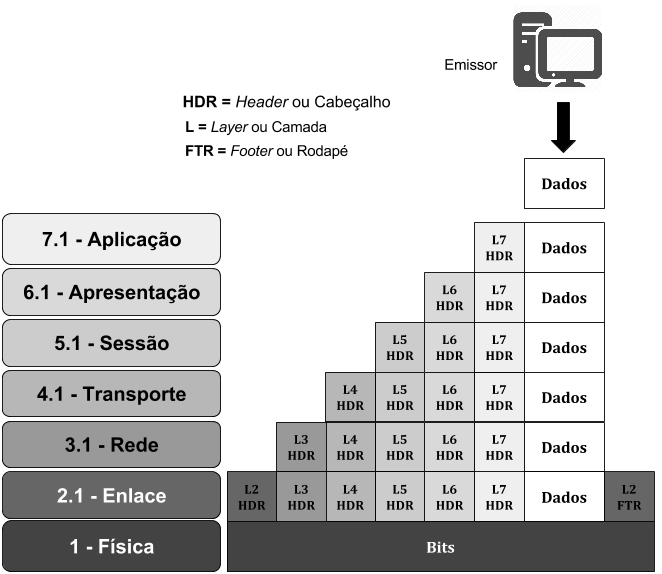
\includegraphics[scale=.5]{figuras/cap2/03EncapsulamentoDedados}
		\caption{\label{fig_3}Encapsulamento de dados}
	\end{figure}	
	
	\par Tomando como base o modelo OSI, o encapsulamento ocorre na seguinte ordem (\autoref{fig_3}):
	
	\begin{enumerate}
		\item Os dados são enviados de uma aplicação para a camada de aplicação.
		\item A camada de aplicação adiciona o seu cabeçalho aos dados. O pacote resultante é passado para a camada de apresentação.
		\item A camada de apresentação adiciona o seu cabeçalho aos dados. O pacote resultante é passado para a camada de sessão.
		\item A camada de sessão adiciona o seu cabeçalho aos dados. O pacote resultante é passado para a camada de transporte.
		\item A camada de transporte adiciona o seu cabeçalho aos dados. O pacote resultante é então passado para a camada de rede.
		\item A camada de rede adiciona o seu cabeçalho aos dados. O pacote resultante é então passado para a camada de enlace.
		\item A camada de enlace adiciona o seu cabeçalho e também o rodapé (chamado de \textit{footer} em inglês) aos dados. Este rodapé contém a checagem da sequência de quadros (FCS ou \textit{Frame Check Sequence}), que é usada pelo destinatário para verificar se há algum erro nos dados. O pacote resultante é então passado para a camada física.
		\item A camada física então transmite os bits para o meio de rede, que pode ser cabeado (fibra ótica, par trançado ou coaxial) ou sem fio(rádio, celular, infravermelho, \textit{Bluetooth}).
	\end{enumerate}

	%INSERIR FIGURA Desencapsulamento de dados
	\begin{figure} [H]
		\centering
		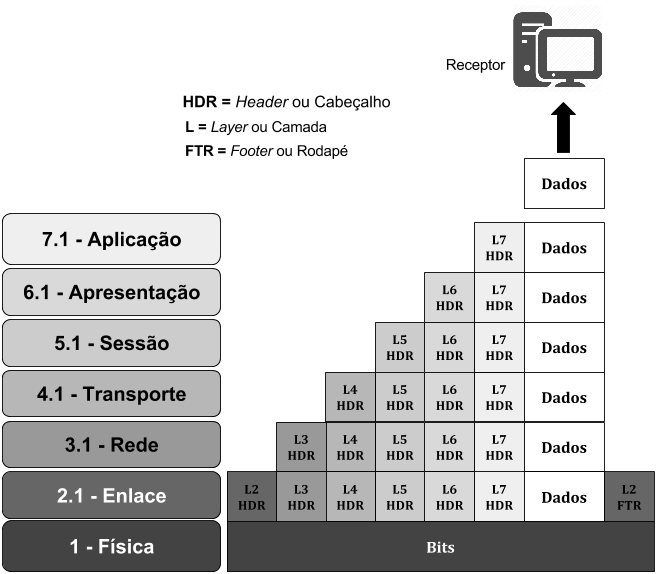
\includegraphics[scale=.5]{figuras/cap2/04DesencapsulamentoDedados}
		\caption{\label{fig_4}Desencapsulamento de dados}
	\end{figure}
	
	\par No desencapsulamento, vemos o processo acontecer de maneira invertida (\autoref{fig_4}).

	\begin{enumerate}
		\item O dispositivo destinatário recebe a sequencia de bits através do meio de rede e sua camada física entrega os bits para a camada de enlace.
		\item A camada de enlace executa as seguintes ações:
		\begin{itemize}
			\item Verifica o rodapé contendo o FCS para a detecção de erros.
			\item Se houver erros nos dados, o pacote pode ser descartado, e a camada de enlace pode solicitar a retransmissão dos dados.
			\item Se não houver erros,  a camada de enlace lê e interpreta as informações de controle no cabeçalho da camada de enlace.
			\item Retira o cabeçalho da camada de enlace e o rodapé, e então passa o restante dos dados até a camada de rede baseando-se nas informações de controle do cabeçalho.
		\end{itemize} 
		\item Das camadas de rede até apresentação os cabeçalhos são retirados e o restante dos dados entregue à camada de aplicação.
		\item A camada de aplicação recebe e interpreta os dados.		
	\end{enumerate}	
	
	\section{\textit{Unicast}, \textit{Multicast} e Broadcast}
	
	\par Existem três diferentes formas de compartilhamento de mensagens, chamados de \textit{Unicast}, \textit{Multicast} e Broadcast. Estes descrevem técnicas específicas para o envio da informação de acordo com cada possível cenário.
	
	\par \textit{Unicast} (\autoref{fig_5}) é o termo utilizado para descrever a comunicação onde uma mensagem é enviada de um ponto à outro. Neste caso, existe apenas um emissor e um destinatário por mensagem.
	
	%INSERIR IMAGEM 5 Unicast
	\begin{figure} [H]
		\centering
		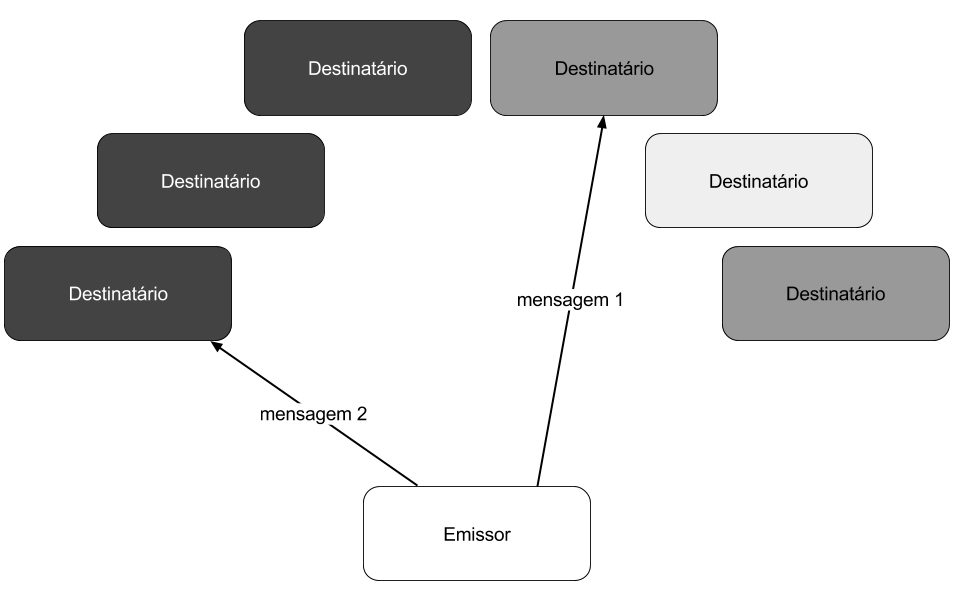
\includegraphics[scale=.45]{figuras/cap2/05Unicast}
		\caption{\label{fig_5}\textit{Unicast}}
	\end{figure}
		
	\par Broadcast (\autoref{fig_6}) representa a comunicação de uma mensagem enviada de um ponto para todos os outros pontos da rede. Neste método, existe apenas um emissor mas a mensagem é enviada para todos os destinatários conectados.
	
	%INSERIR IMAGEM 6 Broadcast
	\begin{figure} [H]
		\centering
		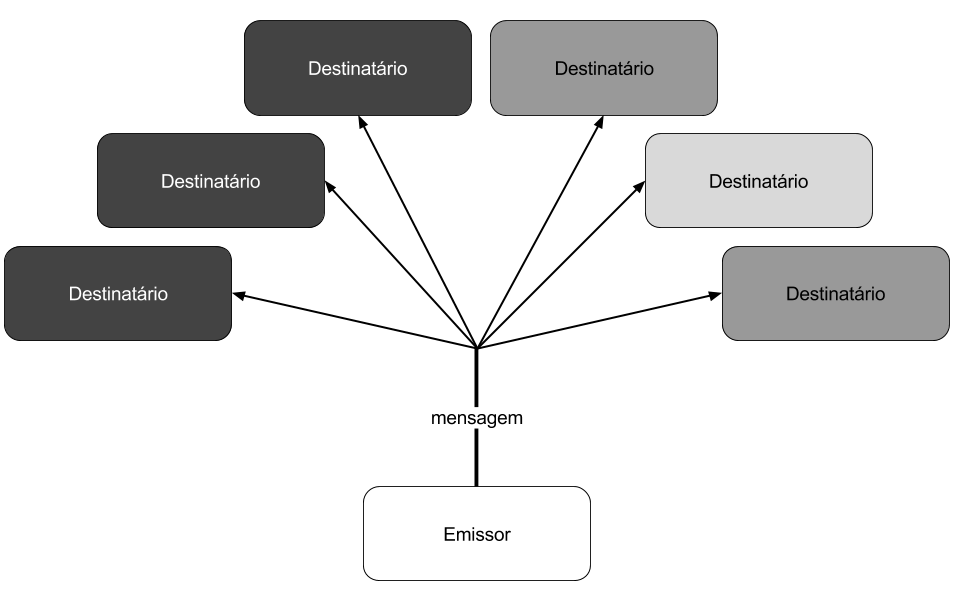
\includegraphics[scale=.45]{figuras/cap2/06Broadcast}
		\caption{\label{fig_6}Brodcast}
	\end{figure}
	
	\par \textit{Multicast} (\autoref{fig_7}) descreve a comunicação onde uma mensagem é enviada de um, ou mais pontos, para um conjunto de outros pontos. Neste método, pode-se ter um ou mais emissores e a mensagem é distribuída para um conjunto de destinatários (pode não existir nenhum destinatário ou qualquer número de destinatários).
	
	%INSERIR IMAGEM 7 Multicast
	\begin{figure} [H]
		\centering
		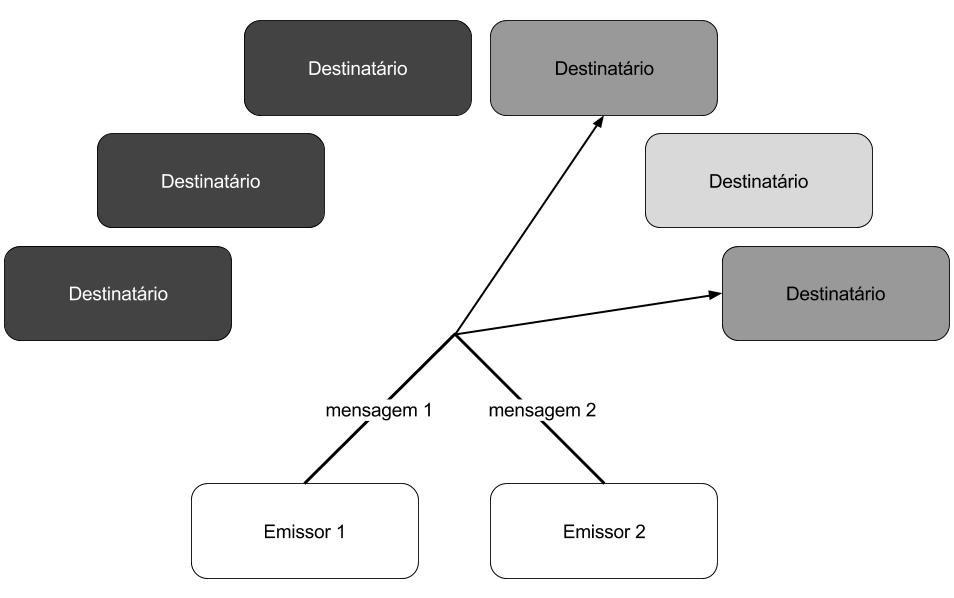
\includegraphics[scale=.45]{figuras/cap2/07Multicast}
		\caption{\label{fig_7}\textit{Multicast}}
	\end{figure}	

	\section{Redes LAN}
	
	\par As redes de comunicação têm geralmente duas categorias primárias, que podem ser diferenciadas pelo seu tamanho e área de cobertura. Existem as redes locais (LAN ou \textit{Local Area Networks}) e as redes de longo alcance (WAN ou \textit{Wide Area Networks}). As redes metropolitanas (MAN ou \textit{Metropolitan Area Networks}) se encaixam como categoria entre as LANs e WANs.
	
	\par As redes locais (LANs) são o tipo mais comum de redes, podendo ser encontradas na maioria das residências, empresas e instituições de ensino. É comumente privada e limitada a alguns poucos quilômetros.
	
	\par As LANs atuais são redes de alta velocidade (entre 100 Mbps a 10 Gbps), baixo índice de erros e cobrem uma área geográfica relativamente pequena (Tanenbaum, 2010). As LANs conectam estações de trabalho, periféricos, roteadores, \textit{switches} e outros dispositivos em um único prédio ou área geográfica. O padrão \textit{Ethernet} é de longe o tipo mais comum de LAN cabeada.
	
	\section{Família de padrões IEEE 802}
	
	\par O conjunto de padrões que lida com as redes LAN é o IEEE 802. Este padrão trata sobretudo das camadas física e de enlace do modelo OSI aplicadas em redes locais.
	
	\par O IEEE por meio do padrão referido subdividiu a camada de enlace em duas subcamadas nomeadas de LLC (\textit{Logical Link Control} ou Controle de Enlace Lógico) e MAC (\textit{Media Access Control} ou Controle de Acesso ao Meio).
	
	\par A subcamada de Controle de Enlace Lógico se localiza abaixo da camada de Rede do modelo OSI. Esta é responsável pelo processo de encapsulamento e desencapsulamento da camada de Enlace, lidando portanto com o controle de fluxo e erros. O cabeçalho criado pelo LLC é quem informa à camada de enlace o que fazer com o pacote quando esta recebe o \textit{frame}. Por exemplo, quando um \textit{host} recebe um \textit{frame}, este olha para o cabeçalho gerado pelo LLC para entender que o pacote está destinado ao protocolo IP na camada de Rede. A subcamada também é responsável pela multiplexação{\footnote{Combinação de dois ou mais canais de informação por apenas um meio de transmissão}} e decodificação de protocolos na camada de enlace.
	
	\par A subcamada MAC age como interface entre a camada LLC e a camada física da rede. O padrão IEEE 802.3 especifica os endereços MAC, que identificam unicamente múltiplos dispositivos da camada de enlace, como as placas de rede. A subcamada MAC mantém uma tabela de endereços MAC (ou endereços físicos) de dispositivos. Cada dispositivo deve ser um endereço MAC único para ingressar na rede.
	
	\par A subcamada MAC é quem provê serviços de comunicação \textit{Unicast}, \textit{Multicast} e \textit {Broadcast}.
	
	\section{Família de padrões IEEE 802.11}
	
	\par As redes Locais utilizam-se de meio cabeado e sem fio para a transmissão de bits entre os dispositivos da rede. As redes sem fio, também conhecidas como Redes \textit{Wifi} ou \textit{Wireless} foram uma grande novidade tecnológica dos últimos anos. A partir de 1997, o IEEE começou a definir uma série de padrões de transmissão e codificação para redes sem fio na família de padrões 802.11, que é aninhada à família de padrões IEEE 802. Como base, o referido padrão trata de especificações ligadas às camadas de rede e de enlace do modelo OSI voltados para Redes sem fio de Área Local (WLAN ou \textit{Wireless Local Area Networks}).
	
	\par Ao longo dos anos, uma miríade de padrões foram adicionados à família 802.11, sendo diferenciados por letras subsequentes ao número da norma. Em cada padrão adicionado à família 802.11, há uma série de especificidades que adequam-se às linhas gerais da norma. Como exemplo, são citadas algumas dessas normas na \autoref{tab_0}.
	
	%INSERIR TABELA padrões IEEE 802.11
	\begin{table}[H]
		\centering
		\renewcommand{\arraystretch}{1.5}
		\begin{tabular}{|c|p{12cm}|} \hline
		\textbf{Padrão IEEE} & \multicolumn{1}{c|}{\textbf{Descrição}} \\ \hline
		802.11a & Padrão de comunicação sem fio baseado na técnica de multiplexação por divisão de freqüência ortogonal (OFDM). Opera na frequência 5.8 GHz e alcança velocidades de até 54 Mbps, porém entrega em média 20 Mbps. Sofre menor interferência de sinal que o padrão 802.11b e possui melhor taxa de transferência.\\ \hline
		802.11b & Padrão de comunicação sem fio que opera na frequência 2.4 GHz usando o mesmo método de acesso ao meio do padrão 802.11 original. A faixa de frequência é a mesma utilizada em \textit{bluetooth}, microondas, celulares e alguns rádio amadores, e por isso sofre relativa interferência. É um dos padrões mais utilizados em roteadores sem fio devido ao baixo custo. Oferece velocidades na média de 11 Mbps.\\ \hline
		802.11e & Agrega Qualidade de Serviço (QoS) as redes 802.11. Permite a transmissão de classes de tráfego diferentes, o que otimiza a utilização da rede.\\ \hline
		802.11g & Utiliza a faixa de 2.4 GHz do 802.11b porém usa a técnica de transmissão OFDM assim como o padrão 802.11a. Também sofre interferências assim como o padrão 802.11b.\\ \hline
		802.11n & Utiliza técnicas de comunicação MIMO aliadas a canais de 40 MHz para entregar taxas de transferência entre 54 a 600 Mbps. Oferece suporte às frequências dos padrões 802.11a e 802.11b.\\ \hline
		802.11p & Emenda que faz parte da família de padrões WAVE. Implementação de redes sem fio para ambientes veiculares que também utiliza a técnica de modulação de sinal OFDM. \\ \hline		
		\end{tabular}
		\caption{\label{tab_0}Padrões IEEE 802.11}
	\end{table}
	
	\subsection{Modos de operação}
	
	\par As redes sem fio suportam basicamente dois modos de operação: Infra-estruturado e ad-hoc.
	
	\par O modo de operação infra-estruturado utiliza de pontos de acesso (\textit{Access Point} ou AP) para controlar os nós cobertos por determinada área geográfica. Como exemplo, na \autoref{fig_8} os nós de rede sem fio se comunicam com outros equipamentos ou com a rede cabeada por meio de um ponto de acesso, que é representado por um roteador sem fio.
	
	% INSERIR FIGURA 08 Modo infra-estruturado
	\begin{figure} [H]
		\centering
		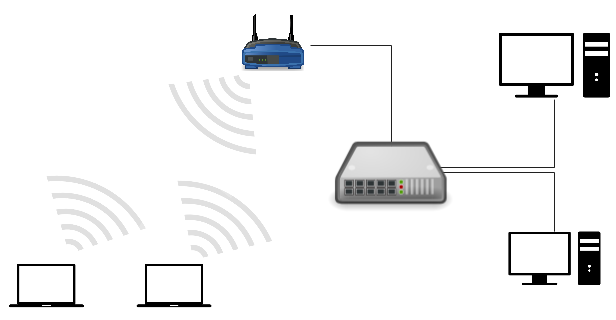
\includegraphics[scale=.5]{figuras/cap2/08ModoInfra-estruturado}
		\caption{\label{fig_8}Modo Infra-estruturado}
	\end{figure}		
	
	\par As Redes \textit{Ad Hoc} se diferenciam por serem redes sem fio onde não há um nó central servindo como ponto de acesso. As estações ou nós comunicam-se como se fossem, ao mesmo tempo, os \textit{hosts} e os roteadores da rede (\autoref{fig_9}).
	
	% INSERIR FIGURA 09 Modo de operação ad-hoc
	\begin{figure} [H]
		\centering
		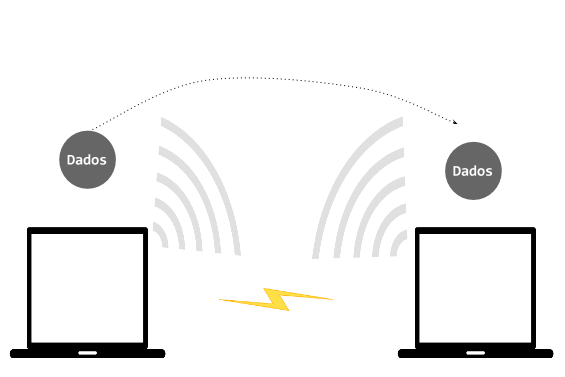
\includegraphics[scale=.3]{figuras/cap2/09ModosdeOperacaoAdHoc}
		\caption{\label{fig_9}Modo de Operação Ad-Hoc}
	\end{figure}
	
	\subsection{Arquitetura IEEE 802.11}
	
	\par Quando duas ou mais estações se comunicam umas com as outras, estas compartilham um Conjunto Básico de Serviços(BSS ou \textit{Basic Service Set}). Um BSS mínimo é formado entre dois nós. As redes locais 802.11 utilizam o BSS como um bloco de construção padrão.
	
	\par O BSS que não se conecta a um AP é chamado de BSS Independente (\textit{Independent} BSS ou IBSS). Este tipo de BSS é comumente visto em Redes \textit{Ad Hoc}. A formação de um IBSS pode ser melhor entendida na \autoref{fig_10}.
	
	% INSERIR FIGURA 10 Redes Ad Hoc - IBSS
	\begin{figure} [H]
		\centering
		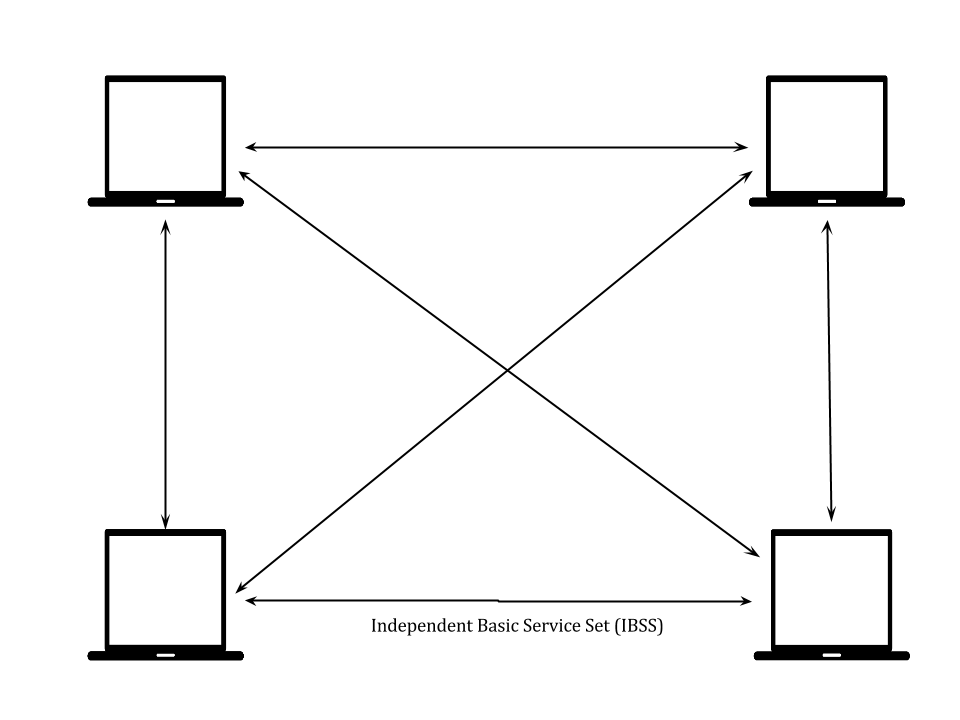
\includegraphics[scale=.35]{figuras/cap2/10ArquiteturaIEEE80211IBSS}
		\caption{\label{fig_10}Arquitetura IEEE 802.11 - IBSS}
	\end{figure}
	
	\par Em redes infra-estruturadas, cada estação conectada ao AP executa o mesmo protocolo MAC e compete pelo acesso ao mesmo meio sem fio compartilhado. O BSS controla o acesso a recursos e serviços do AP, filtrando os quadros transmitidos por outras estações que não pertencem ao BSS. Um BSS pode estar isolado ou pode se conectar a outro BSS utilizando um DS (\textit{Distribution System} ou Sistema de Distribuição). O ponto de acesso funciona como uma ponte neste caso. O conceito de DS aumenta a cobertura da rede, fazendo com que cada BSS se torne uma extensão de uma rede ainda maior.
	
	% INSERIR FIGURA 11 Redes Infra-estruturadas - BSS
	\begin{figure} [H]
		\centering
		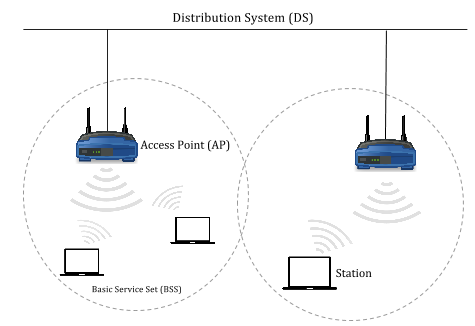
\includegraphics[scale=.6]{figuras/cap2/11ArquiteturaIEEE80211BSS}
		\caption{\label{fig_11}Arquitetura IEEE802.11 - BSS}
	\end{figure}
	
	\par Para entrar em um BSS, a estação deve primeiramente "ouvir" a frequência transmitida pelo ponto de acesso, e depois executar diversos passos que incluem processos de autenticação e associação. Os usuários de redes sem fio 802.11 identificam a presença de um BSS por meio do SSID (\textit{Service Set Identification} ou Identificação de Conjunto de Serviços) que é anunciado pelos transmissores sem fio. As interfaces de rádio identificam um BSS no nível da subcamada MAC por intermédio de seu BSSID (BSS \textit{Identification} ou Identificação BSS), que é um campo da dispositivo transmissor com formato de endereço MAC.
	
	\par Cada BSS deve ser identificado por um BSSID único, que em uma rede infraestruturada é frequentemente escolhido como o endereço MAC do ponto de acesso. Em um BSS Independente, normalmente é utilizado um endereço MAC administrado localmente, formado por um numero aleatório de 46 bits, e 2 bits identificando o endereço como “individual” (em vez de “grupo”) e “local” (em vez de “universal”). Ademais, o padrão IEEE 802.11 define um BSSID especial, com todos os 48 bits tendo valor binário 1.
	
	\subsection{Serviços IEEE 802.11}
	
	\par O IEEE define diversos serviços que precisam ser fornecidos pela LAN para prover funcionalidade equivalente às LANs cabeadas. Os serviços mais importantes são:
	
	\par \textbf{O serviço de Associação} estabelece uma associação inicial entre uma estação e um ponto de acesso. Antes que uma estação possa transmitir ou receber quadros em uma WLAN, sua identidade e endereço precisam ser conhecidos. Para esse fim, uma estação precisa estabelecer uma associação com um ponto de acesso. O ponto de acesso pode, então, comunicar essas informações com outros pontos de acesso para facilitar o roteamento e a entrega dos quadros endereçados.
	
	\par \textbf{O serviço de Reassociação} torna possível uma associação estabelecida transferir-se de um ponto de acesso para outro, permitindo o deslocamento de uma estação móvel.
	
	\par \textbf{O serviço de Desassociação} emite uma notificação por parte de uma estação ou de um ponto de acesso de que uma associação existente está terminada. Uma estação deve emitir esta notificação antes de deixar uma área ou de desligar. Entretanto, o recurso de gerenciamento do MAC se protege contra estações que desaparecem sem notificação.
	
	\par \textbf{O serviço de Autenticação} é usado para estabelecer identidade entre estações. Em uma LAN cabeada, geralmente se considera que o acesso a uma conexão física significa autorização para se conectar com a LAN. Essa não é uma suposição válida para uma LAN sem fio, na qual a conectividade é obtida simplesmente com uma antena corretamente sintonizada. O serviço de autenticação é usado pelas estações para estabelecer sua identidade em estações com as quais ela deseja se comunicar. O padrão não exige qualquer esquema de autenticação específico, que poderia variar de um protocolo relativamente inseguro a esquemas de criptografia de chave pública.
	
	\par \textbf{O Serviço de Privacidade} é usado para impedir que o conteúdo das mensagens seja lido por outras pessoas além do destinatário pretendido. O padrão sugere o uso opcional da criptografia para garantir privacidade.		
	
	\section{Redes Ad-hoc Móveis}
	
	\par As redes \textit{ad hoc} se destacam por serem redes onde não há um nó central - como um roteador ou um \textit{switch} - servindo como ponto de acesso. Os nós funcionam de forma similiar a roteadores. Estes nós que se conectam consomem e geram dados, assim como armazenam e entregam informações. Em redes \textit{ad hoc} são trocados quadros de arquitetura IBSS, se diferenciando das redes de infraestrutura, que utilizam quadros BSS. Além disso, as redes \textit{ad hoc} não possuem conexão direta com a Internet. Justamente por serem redes sem infraestrutura, as mesmas não possuem provedor de acesso.
	
	\par As redes sem fio de nós móveis que estão próximos uns aos outros são chamadas de MANETs (\textit{Mobile Ad Hoc Networks} ou Redes \textit{Ad Hoc} Móveis). Estes nós podem ser \textit{notebooks}, \textit{tablets}, \textit{smartphones}, etc. Por possuírem dispositivos que se movem constantemente, as MANETs estão sujeitas à constantes variações na topologia de rede, com nós que podem entrar e sair da rede em um curto intervalo de tempo, ocasionando a alteração rápida de rotas. 
	
	\par O roteamento de pacotes em redes \textit{ad hoc} é mais complexo do que em redes infraestruturadas e possui uma série de desafios. Para rotear os pacotes, os desafios encontrados são: mobilidade dos nós que impactam diretamente as rotas, implantação de Qualidade de Serviço (QoS) para os fluxos de aplicações multimídia e a escalabilidade da rede. Há também desafios com relação ao consumo de energia elétrica que os nós dispõem para realizar a transmissão e recepção dos dados além de realizar outros processos. Como a troca de informações entre os nós é intensa, a energia é gasta de maneira mais acelerada. Desafios que envolvem conectividade também preocupam. As redes \textit{ad hoc} apresentam condições inconstantes como taxas de erro de bit variáveis e interferências na comunicação por outros meios de transmissão.
	
	\par Ao longo dos anos, diversos protocolos de roteamento para MANETs foram criados. Seguindo uma primeira abordagem, os protocolos de redes \textit{ad hoc} móveis foram classificados baseando-se na topologia (Royer \& Toh, 1999) ou na posição (Giordano et al., 2004). Os protocolos baseados na topologia ainda podem ser subclassificados como pró-ativos, reativos e híbridos enquanto os protocolos baseados em posição podem ser classificados em roteamento guloso ou restrito. Alguns exemplos de protocolo são citados e categorizados na \autoref{fig_12}.
	
	% INSERIR FIGURA 12 Protocolos de roteamento de MANETs
	\begin{figure} [H]
		\centering
		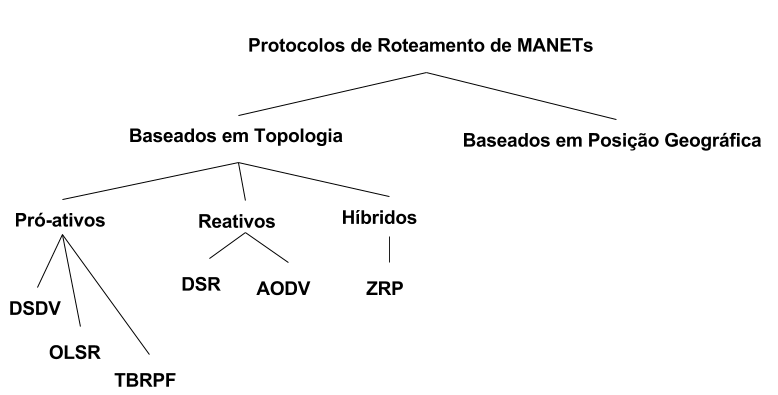
\includegraphics[scale=.5]{figuras/cap2/12ProtocolosDeRoteamentoMANETs}
		\caption{\label{fig_12}Protocolos de Roteamento em MANETs}
	\end{figure}	
	
	\par Não é de escopo deste trabalho abordar os detalhes dos protocolos mostrados, entretanto é importante salientar que o estudo de protocolos das MANETs serviu de base para o desenvolvimento do estudo das redes veiculares, principal tema deste trabalho. 
	

	%--------------------------------------------------------------
	
	\newpage
	\chapter{Redes de Comunicação Veiculares}

	\par Segundo a Organização Mundial de Saúde(OMS), acidentes de carro estão entre as 10 maiores causa de morte no mundo{\footnote{http://www.who.int/mediacentre/factsheets/fs310/en/ (acesso em 22 de jun. 2016)}}. Conforme relatado pela Universidade de Stanford, mais de 90\% dos acidentes têm origem em falha humana{\footnote{http://cyberlaw.stanford.edu/blog/2013/12/human-error-cause-vehicle-crashes (acesso em 25 de jun. 2016)}}. Tais dados são alarmantes para a sociedade visto que nenhum meio de transporte tira tantas vidas como o meio rodoviário.

	\par Se comparados com transporte de outros meios, os transportes terrestres são os menos seguros. Os outros meios, como o aquático, aéreo e ferroviário, sofrem menos acidentes porém eventuais catástrofes assumem maiores proporções por justamente serem transportes de massa. Estes meios de transporte entenderam melhor a carência de segurança na locomoção e por isso há algumas décadas vemos navios e aviões equipados com sistemas de comunicação utilizando transponders, que auxiliam na prevenção de acidentes e na escolha de novas rotas, seja por tráfego denso ou por condições climáticas adversas. Nos trens, o uso de tecnologias 3G e 4G pelos sistemas de comunicação também tem sido fundamental para proporcionar o aumento da segurança e da pontualidade nas ferrovias metropolitanas e intercidades.
	
	\par Atualmente, os condutores de veículos terrestres contam com itens de proteção como cintos de segurança, \textit{airbags}, sensores de obstáculo, alarmes de velocidade, e outros equipamentos. Contudo, alguns destes itens não têm provocado um efeito de compra pelos motoristas (pelo seu preço adicional em veículos novos) e muito menos causado uma substancial diminuição no número de acidentes. Segundo prevê a OMS, acidentes automobilísticos passarão da 9ª para a 7ª maior causa de morte de humanos entre todas as idades em 2030 (\textit{Global Status Report on Road Safety}, 2015). Por isto, governos e grandes empresas continuam a trabalhar no desenvolvimento de tecnologias para aumento da segurança veicular. O potencial advento de sistemas de comunicação entre veículos representa o próximo passo na evolução da segurança veicular, possibilitando a interação entre diferentes veículos para evitar acidentes. Segundo Yang et al (2014), os principais objetivos desses sistemas são (1) oferecer conectividade ubíqua para os usuários e (2) possibilitar a comunicação de veículo para veículo, oferecendo condições necessárias para que aplicações com diferentes requisitos sejam atendidas satisfatoriamente. Tais aplicações compõem um ITS (\textit{Intelligent Transportation System} ou Sistema de Transportes Inteligente). Exemplos destas aplicações incluem monitoração cooperativa do tráfego, controle de fluxos de tráfego, auxílio a cruzamentos sem sinalização, prevenção de colisões, propagação de mensagens de emergência, serviços de informação próximos, etc.
	
	\par Os sistemas de comunicação entre veículos formam as chamadas redes veiculares. Estas redes são compostas por veículos e equipamentos fixos geralmente localizados às margens de estradas ou de ruas. As redes veiculares se diferenciam de outras redes sem-fio principalmente pela natureza dos nós, que são compostos por veículos com interfaces de comunicação sem-fio, e por equipamentos fixos nos entornos das vias. 
	
	\par As redes veiculares possuem um conjunto de desafios para sua adoção em larga escala. De início, percebemos que os nós destas redes apresentam alto grau de mobilidade e limitam-se a trajetórias em vias públicas de acesso. Além disso, verifica-se o dinamismo dos cenários e a escalabilidade em termos do número de nós na rede. A perda de conectividade durante a transmissão de dados e o tempo reduzido em que os nós permanecem em contato são outros desafios. 
	
	\par Neste capítulo, veremos  o desenvolvimento das Redes Veiculares e os padrões que foram criados para sua eventual consolidação de mercado.
	
	\section{História}
	
	\indent Os primeiros estudos em comunicação veicular iniciaram no começo dos anos 80 quando o governo do Japão instou a JSK (Associação de Tecnologia Eletrônica de Tráfego de Automóvel e de Condução) a iniciar estudos sobre o desenvolvimento de Sistemas de Transporte Inteligentes. Alguns anos depois, o congresso americano ordenou a criação de um programa chamado IVHS (\textit{Intelligent Vehicle Highway System} ou Sistema de Rodovia Veicular Inteligente) baseado no ato pela Eficiência dos Transportes de Superfície (\textit{Intermodal Surface Transportation Efficiency} - ISTEA) de 1991. Depois, os programas de pesquisas americano PATH (da Universidade da Califórnia) e europeu CHAUFFEUR demonstraram técnicas para acoplamento eletrônico de veículos. 
	
	\par No início dos anos 2000, um projeto europeu chamado CarTALK2000 foi lançado com objetivo de investigar soluções relacionadas a condução confortável e segura baseada em comunicação interveicular. Nos últimos anos, sendo impulsionados pelos padrões de interfaces sem fio IEEE 802.11, o número de pesquisas na área de comunicação interveicular aumentou consideravelmente. Além disso, grandes empresas automobilísticas começaram a se interessar pelo assunto formando um consórcio sem fins lucrativos chamado Car2Car que tem por objetivo reforçar a eficiência e segurança no tráfego rodoviário, utilizando-se da comunicação interveicular (V2V) e contando com o amparo de infraestruturas de acostamento (V2I). Empresas como Audi, BMW, Ford, Hyundai, Jaguar, Renault, Volkswagen, Volvo e Yamaha são membros deste consórcio.
	
	\section{VANETs}
	
	\par Nos últimos anos, com o avanço no estudo das MANETs, foi iniciado o estudo em massa das redes móveis no campo interveicular. As VANETs começaram então a ser desenvolvidas, funcionando como um tipo de MANET de larga escala, tornando veículos em nós de rede sem fio. No entanto, algumas características diferenciam as VANETs das MANETs, tais quais:
	
	\begin{itemize}
		\item Nas VANETs (\autoref{fig_15}), há uma maior restrição das trajetórias em que os nós podem percorrer, visto que os veículos só podem trafegar ruas, avenidas e rodovias.
		\item Não há problemas com relação à energia, já que a energia não é um fator crítico em automóveis, como pode ser para outros tipos de sensores.
	\end{itemize}
	
	% INSERIR Figura 15 Vanets
	\begin{figure} [H]
		\centering
		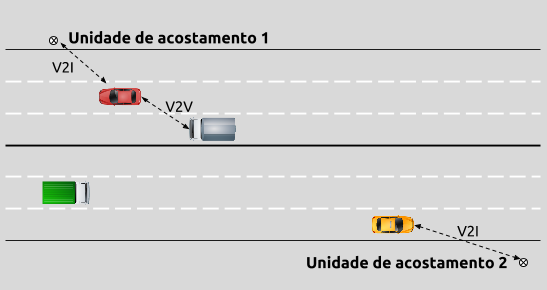
\includegraphics[scale=.7]{figuras/cap3/15VANETs}
		\caption{\label{fig_15}VANETs}
	\end{figure}
	
	\par Com a maior atenção de pesquisadores, o estudo das VANETs foi se aprimorando, de maneira que as organizações responsáveis pela padronização de tecnologias montaram equipes para discutir normas que regimentassem a forma com que as comunicações veiculares seriam utilizadas.
	
	\par A normalização das redes veiculares iniciou-se em 2006, com o desenvolvimento da família de padrões WAVE. Estes padrões serão vistos em maior detalhe nos próximos capítulos.
	
	\section{Dispositivos Car2X: Componentes e Tipos de Comunicação}
	
	\par Um dispositivo Car2X é um meio de comunicação de rádio que pretende oferecer serviços interoperáveis para os transportes. Funciona como um “roteador” para veículos. Pode apenas transmitir ou receber de dados (\textit{Simplex}) ou realizar ambas as operações.
	
	\par Atualmente, várias empresas produzem hardware, \textit{firmware} e software para dispositivos de tecnologia Car2X. Entre elas, se destacam a Cohda Wireless, Autotalks, Commsignia, Rohde \& Schwarz, Vector Informatik e Unex.
	
	Os dipositivos Car2X produzidos atualmente por estas empresas são unidades de bordo e unidades de acostamento.
	
	\par As \textbf{unidades de bordo} são dispositivos de rede veicular usados por objetos móveis no trânsito. Podem ser desde veículos até unidades portáteis de sinalização ou unidades para pedestres (como trabalhadores em uma rodovia). Também são chamadas de \textit{On Board Equipments} (OBE) ou \textit{On-Board Units} (OBU). Podem se comunicar com outros dispositivos Car2X estáticos ou móveis. A \autoref{OBU_Cohda} mostra um exemplo de unidade de bordo produzida pela empresa Cohda Wireless.
	
	% INSERIR Figura 15 Vanets
	\begin{figure} [H]
		\centering
		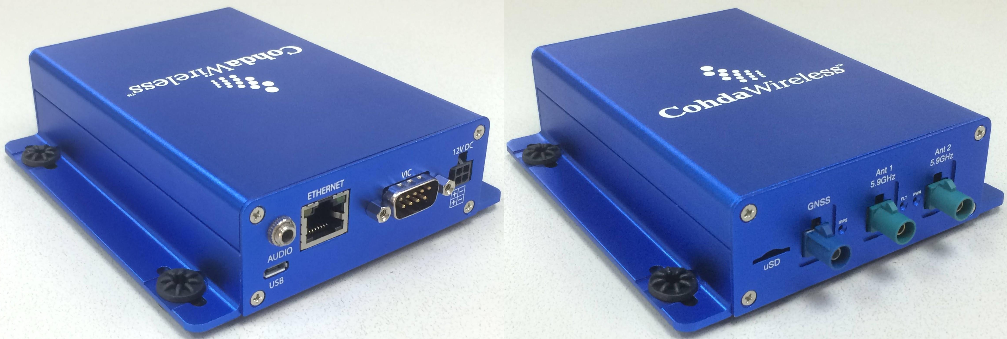
\includegraphics[scale=.45]{figuras/waveDevices/CohdaOBU}
		\caption{\label{OBU_Cohda}OBU produzida pela Cohda Wireless}
		\legend{Fonte: \href{http://cohdawireless.com/Products/Hardware}{http://cohdawireless.com/Products/Hardware} (acesso em 22 de set. 2016)}
	\end{figure}	
	
	\par As \textbf{unidades de acostamento} são dispositivos de rede veicular estáticos instalados ao lado de rodovias ou avenidas (num poste de luz, semáforo ou ponto de pedágio). Também chamados de \textit{Road Side Equipments} (RSE) ou \textit{Road Side Units} (RSU). Podem estar conectadas a uma rede de infraestrutura. Podem se comunicar com outros dispositivos Car2X estáticos ou móveis. A \autoref{RSU_Cohda} mostra um exemplo de unidade de acostamento produzida pela empresa Cohda Wireless.
	
	\begin{figure} [H]
		\centering
		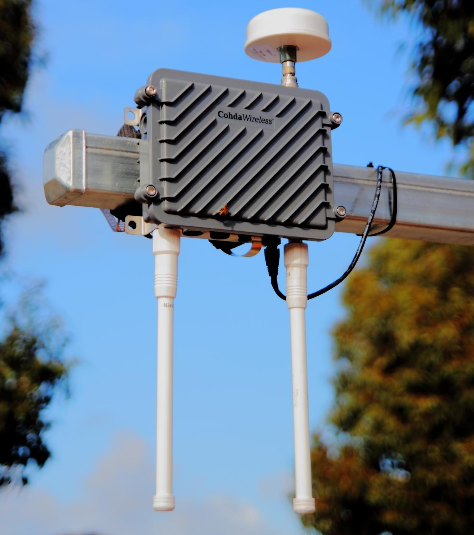
\includegraphics[scale=.45]{figuras/waveDevices/CohdaRSU}
		\caption{\label{RSU_Cohda}RSU produzida pela Cohda Wireless}
		\legend{Fonte: \href{http://cohdawireless.com/Products/Hardware}{http://cohdawireless.com/Products/Hardware} (acesso em 22 de set. 2016)}
	\end{figure}
	
	\par Os dispositivos Car2X têm duas principais formas de comunicação: veículo para veículo e veículo para infraestrutura.
	
	\par As comunicações de \textbf{veículo para veículo} (\textit{Vehicle to Vehicle} ou V2V) são transferências de informação apenas entre unidades de bordos de veículos. O protocolo WSMP é o que provê conexões para este tipo de comunicação no padrão IEEE 1609 WAVE.
		
	\par As comunicações de \textbf{veículo para infraestrutura} (\textit{Vehicle to Infrastructure} ou V2I) são as trocas de informações entre unidades de bordo e unidades de acostamento. É possível que uma unidade de acostamento conecte-se a uma rede de infraestrutura, o que poderia prover conexão à Internet as unidades de bordo próximas.
	
	\par A \autoref{fig_16} exemplifica um cenário de comunicações V2V e V2I contendo OBUs e RSUs.
	
	%INSERIR FIGURA 16 Diversas RSUs e OBUs
	\begin{figure} [H]
		\centering
		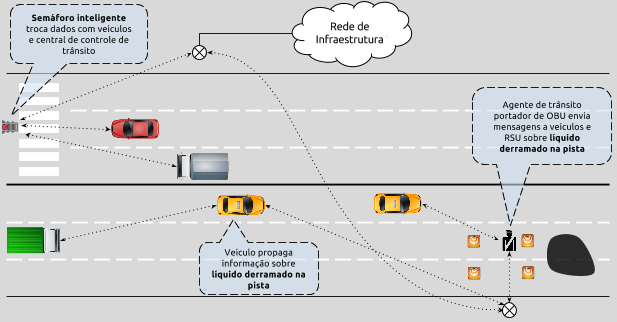
\includegraphics[scale=.7]{figuras/cap3/16DiversasOBUsERSUs}
		\caption{\label{fig_16}Diversas OBUs e RSUs}
	\end{figure}
	
	\section{Família de padrões WAVE}
	
	\par A padronização das redes veiculares tem sido feita por dois grandes grupos: pelo IEEE, numa colaboração entre a Sociedade de Tecnologia Veicular e o Comitê de Sistemas de Transportes Inteligentes, e pelo ETSI (\textit{European Telecommunications Standards Institute} ou Instituto Europeu de Padrões de Telecomunicações), por intermédio de seu Comitê de Transportes Inteligentes. Cabe ressaltar que este trabalho seguirá as diretrizes dos padrões IEEE 1609, visto que as normas ETSI são voltadas a atender principalmente o mercado europeu.
	
	\par A família de normas IEEE destina-se a prover um conjunto padronizado de interfaces para que diferentes fabricantes de automóveis possam fornecer comunicações V2V e V2I, garantindo a interoperabilidade entre os dispositivos fabricados.
	
	\par Para ajustes na camada física e de enlace lógico, o IEEE adicionou uma emenda à família de padrões 802.11 (denominada 802.11p) para especificar as mudanças nas configurações de redes sem fio adaptando-se ao meio veicular. Esta emenda visa realizar o estabelecimento da conexão mais rápida entre os nós da rede, visto que as altas velocidades de deslocamento dos nós no meio veicular demandam um tempo mais curto para a conexão.
	
	% INSERIR Figura 17 Arquitetura WAVE - Planos
	\begin{figure} [H]
		\centering
		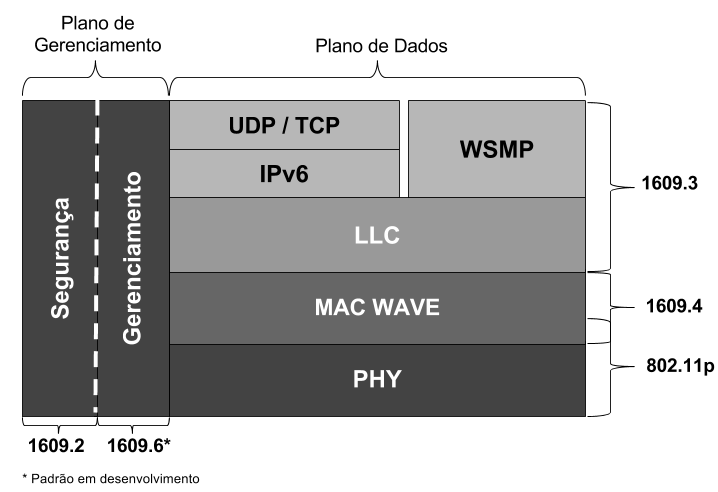
\includegraphics[scale=.6]{figuras/cap3/17ArquiteturaWAVEPlanos}
		\caption{\label{fig_17}Arquitetura WAVE - Planos}
	\end{figure}

	\par A \autoref{fig_17} mostra a divisão de camadas do padrão WAVE em dois componentes abstratos, chamados de Plano de Gerenciamento e Plano de Dados. É necessário delimitar o escopo de atuação de cada um destes componentes.
	
	\par O Plano de Gerenciamento é um componente abstrato da arquitetura WAVE que contém funções que gerenciam entidades no Plano de Dados. Estas funções atuam de forma indireta no transporte de dados de aplicação. O Plano de Gerenciamento pode utilizar camadas inferiores do Plano de Dados a fim de transferir informações de Gerenciamento entre os dispositivos WAVE (Maiores detalhes sobre o plano de gerenciamento na \autoref{sec:PlanGere}).
	
	\par O Plano de Dados é também um componente abstrato da arquitetura WAVE que possui entidades que trocam dados. O Plano de Dados contém um conjunto definido de protocolos de comunicação que transportam dados de gerenciamento e aplicação que podem ser transferidos entre dispositivos WAVE.
	
	\par Também são evidenciadas na \autoref{fig_17} a divisão de normas para as camadas da pilha WAVE. Estes padrões serão abordados ao longo deste trabalho.
	
	\par Além das camadas, alguns padrões da família 1609 definem outras características, como segurança e gerenciamento para aplicações DSRC (\textit{Dedicated Short Range Communications} ou Comunições Dedicadas de Curto Alcance). Na \autoref{tab_1}, a família de padrões WAVE é detalhada. 
	
	% INSERIR Tabela de padrões WAVE
	\begin{table}[H] %[?] Arrumar alinhamento vertical e quebra de linhas (exemplo: quebrar o camadas\\fisica e mac)
		\centering
		\renewcommand{\arraystretch}{1.2}
		\begin{tabular}{|p{1.5cm}|p{2.3cm}|p{8.5cm}|p{2cm}|} \hline
			\textbf{Padrão} & \multicolumn{1}{c|}{\textbf{Área}} & \multicolumn{1}{c|}{\textbf{Descrição}} & \multicolumn{1}{c|}{\textbf{Status}} \\ \hline
			802.11p & Camadas\newline Física e MAC & Emenda que descreve as diferenças específicas na camada física e controle de acesso ao meio em ambientes de comunicação WAVE & Ativo \\ \hline
			1609.0 & Arquitetura & Descreve a arquitetura e os serviços necessários para dispositivos WAVE multicanal & Ativo \\ \hline
			1609.1 & Gerenciador de Recursos & Aplicação retirada que permitia a sites remotos se comunicarem com OBUs via RSUs. & Retirado \\ \hline
			1609.2 & Serviços de Segurança & Define métodos para tornar as mensagens de gerenciamento e aplicação seguras. Descreve funções administrativas necessárias para suporte de funções de segurança. & Ativo \\ \hline
			P1609.2a & Emenda à 1609.2 para gerenciamento de certificados & Descreve como os serviços de segurança WAVE respeitam a privacidade do usuário. Provê características adicionais de gerenciamento de certificação. & Em desenvolvimento \\ \hline
			1609.3 & Serviços de Rede & Especifica protocolos das camadas de rede e transporte e serviços que suportam operações multicanal. & Ativo \\ \hline
			1609.4 & Operação Multicanal & Especifica as funções e serviços da subcamada de Controle de Acesso ao Meio (MAC) que suportam operações multicanal. & Ativo \\ \hline
			1609.5 & Gerente de Comunicação & Padrão previsto para definir serviços de gerenciamento de Comunicação no suporte à conexão entre OBUs e RSUs. & Rascunho \\ \hline
			P1609.6 & Serviços de Gerenciamento Remoto & Padrão em desenvolvimento que define formatos específicos de mensagens de gerenciamento e de dados para dispositivos WAVE remotamente controlados. & Em desenvolvimento \\ \hline
			1609.11 & Protocolo de pagamentos eletrônicos & Define um nível básico de interoperabilidade técnica para equipamentos de pagamento eletrônico. Ex.: OBUs e RSUs usando DSRC & Ativo \\ \hline
			1609.12 & Alocações de Identificadores & Especifica a alocações de identificadores WAVE. & Ativo \\ 
			\hline
		\end{tabular}
			\caption{\label{tab_1}Família de Padrões WAVE}
	\end{table}
	
	
	\section{Plano de Gerenciamento}
	\label{sec:PlanGere}
	
	\par As camadas de gerenciamento e segurança em conjunto formam o que é chamado de forma abstrata de Plano de Gerenciamento WAVE.
	
	\par Os serviços do plano de gerenciamento estão associados com várias entidades do plano de dados para desempenhar funções específicas de camadas que são necessárias à operação do sistema WAVE.
	
	\subsection{Camada de Gerenciamento}
	
	\par A camada de Gerenciamento contém um grupo de entidades conceituais que coordena as operações e as chamadas de funções no Plano de Dados. Estas entidades são citadas na \autoref{tab_2}.
		
	% INSERIR Tabela Entidades de Gerenciamento
	\begin{table}[h] %[?] CUIDADO, ta tirando da posicao?
		\centering
		\renewcommand{\arraystretch}{1.5}
		\begin{tabular}{|c|p{3.4cm}|p{6.7cm}|p{1.5cm}|} 
			\hline
			\textbf{Camada} & \multicolumn{1}{c|}{\textbf{Entidades}} & \multicolumn{1}{c|}{\textbf{Descrição}} & \textbf{Padrões} \\ \hline
			Física & PLME & Entidade que coordena conjunto de funções da camada física e contém interfaces de serviço. & 802.11 \\
			\hline
			\multirow{2}{*}{Enlace - MAC} & MLME & Entidade que coordena conjunto de funções da subcamada MAC e contém interfaces de serviços. Como exemplo, controla o acesso a canais de rádio específicos. Possui MIB. & 802.11 \\ \cline{2-4} 
			& MLMEX & Entidade estendida que coordena outro conjunto de primitivas da subcamada MAC. & 1609.4 \\ \hline
			Enlace - LLC & \multirow{3}{\linewidth}{WME} & \multirow{3}{\linewidth}{Provê funções de Serviços de Rede WAVE. Fornece interfaces de gerenciamento para as entidades do plano de dados.} & \multirow{3}{\linewidth}{1609.3} \\ \cline{1-1} 
			%Enlace - LLC & \multirow{3}{*}{WME} & \multirow{3}{\linewidth}{Conjunto de funções necessárias para prover Serviços de Rede WAVE. Fornece interfaces de gerenciamento para todas as entidades do plano de dados.} & \multirow{3}{\linewidth}{IEEE 1609.3 - 2016} \\ \cline{1-1} 
			Rede & & & \\ \cline{1-1}
			Transporte & & & \\ \hline 
			Aplicação & Gerenciamento de Camadas Superiores & Entidades como SDEE trabalham com primitivas na camada de aplicação. & 1609.0 \\ \hline
			Segurança & Gerenciamento de Serviços de Segurança (SSME) & Entidade responsável pelo gerenciamento as informações de certificados em um dispositivo. & 1609.2 \\
			\hline			
		\end{tabular}
			\caption{\label{tab_2}Entidades de Gerenciamento}
	\end{table}
	
	\par As entidades WME e MLMEX (MLME \textit{Extension} ou Extensão MLME) herdam aspectos da SME (\textit{Station Management Entity} ou Entidade de Gerenciamento de Estação), estabelecida no padrão 802.11.
	
	\subsection{Camada de Segurança}
	
	\par Também residindo no plano de gerenciamento, a camada de segurança pode ser chamada pela WME ou por outras entidades de camadas superiores.
	
	\par O escopo da camada de segurança em dispositivos WAVE é discutido no padrão IEEE 1609.2 - Serviços de Segurança para Aplicações e Mensagens de Gerenciamento, que tem os propósitos de estabelecer a privacidade nas comunicações WAVE e proteger os dispositivos WAVE de ataques e de vazamento de informações.

	\par Segundo a intenção dos padrões IEEE 1609, qualquer dispositivo WAVE deve proteger a privacidade de seus dados, de modo que partes não-autorizadas não conheçam dados pessoais e partes autorizadas conheçam apenas se consentidas para tal.

	\par De modo detalhado, a norma IEEE 1609.2 descreve os seguintes serviços de segurança para aplicações e mensagens de gerenciamento:

	\begin{itemize}
		\item Serviços de Segurança Internos:
		\begin{itemize}	
			\item Serviços de Dados Seguros (SDS)
			\item Gerenciamento Seguro
		\end{itemize}
		\item Serviços de Segurança de Camadas Superiores:
		\begin{itemize}	
			\item Entidade de Verificação de Listas de Revogação de Certificado
			\item Entidade de Distribuição de Certificados Ponto-a-Ponto
		\end{itemize}		
	\end{itemize}

	% INSERIR Figura 18 Segurança WAVE em detalhes
	\begin{figure} [H]
		\centering
		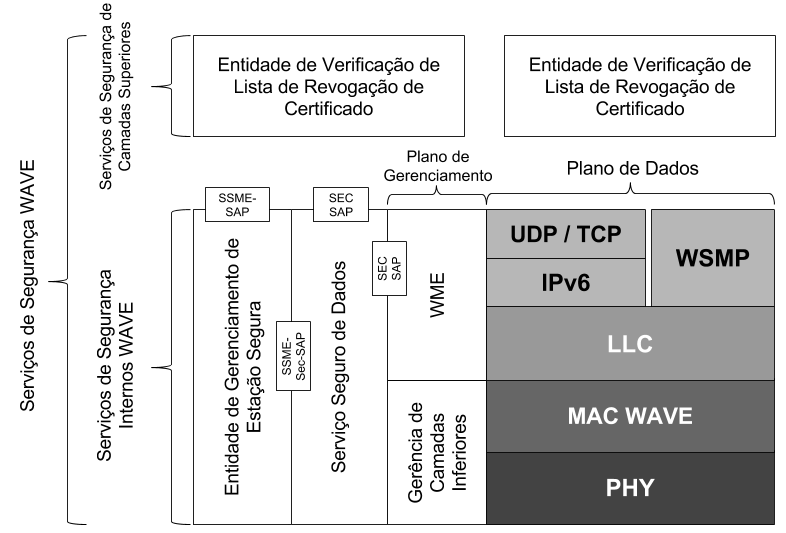
\includegraphics[scale=.5]{figuras/cap3/18SegurancaWAVEDetalhada}
		\caption{\label{fig_18}Segurança WAVE Detalhada}
	\end{figure}

	\par A camada de segurança WAVE gerencia a validação de certificados de segurança,  a criação de unidades de protocolo de dados seguros (SPDU ou \textit{Secure Protocol Data Unit}), além de operações de criptografia. Nas operações de criptografia, a norma cita algoritmos de assinatura, algoritmos hash, algoritmos de chave simétrica e assimétrica, além de diferentes abordagens de chaves de criptografia.

	\par Não é de objetivo deste trabalho discorrer de maneira detalhada sobre o estudo de segurança das redes WAVE, e sim citar a existência da camada e realizar uma abordagem geral.

	\subsection{Interfaces}
	\label{sec:Interfaces}

	\par Para comunicação entre diversos protocolos no Plano de Dados, é necessário ter interfaces. As interfaces nos componentes WAVE são chamados de Pontos de Acesso de Serviços (\textit{Service Access Points} ou SAP). Assim como no modelo OSI, os SAPs do plano de dados se localizam conceitualmente entre uma camada OSI e outra adjacente. No plano de gerenciamento, os SAPs podem ser acessados por quaisquer entidades.

	% INSERIR Figura 19 Service Access Points
	\begin{figure} [H]
		\centering
		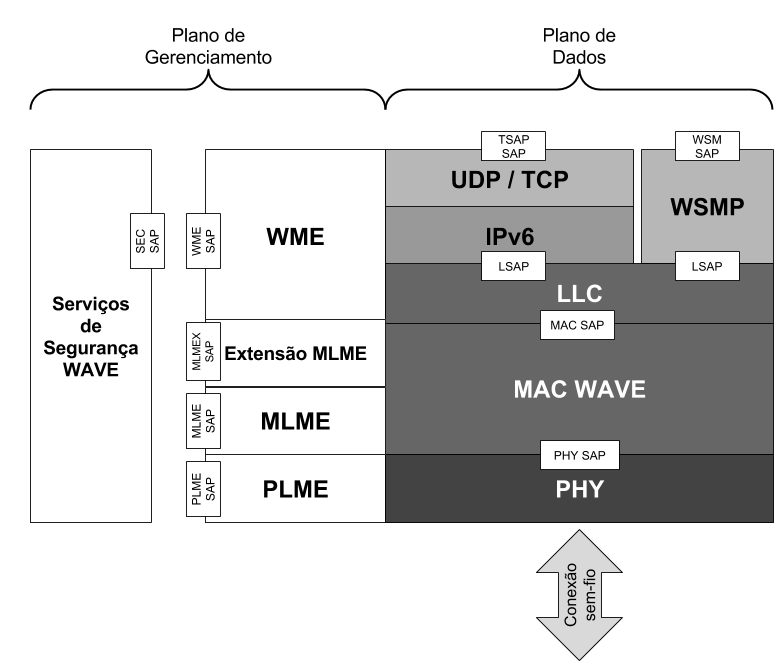
\includegraphics[scale=.5]{figuras/cap3/19ServiceAccessPoints}
		\caption{\label{fig_19}\textit{Service Access Points}}
	\end{figure}

	\par Os SAPs são compostos de primitivas de serviço. Estas primitivas informam ao serviço como desempenhar uma determinada ação. Primitivas de serviço se parecem com procedimentos em linguagem de programação. As primitivas de serviço são “codificadas” na notação ASN.1 (Ver \autoref{ASN1}).

	\section{Camada Física}

	\par A camada física do modelo WAVE foi descrita pelo padrão 802.11p, que é uma emenda à família de padrões 802.11. Esta emenda propõe uma adaptação das redes sem fio em suas camadas física e de enlace (subcamada MAC) para o ambiente veicular.

	\par Os meios sem fio de transmissão de dados mais utilizados na norma 802.11 baseiam-se em Rádio Frequência (RF).  Existem outros meios de propagação sem fio como o Infravermelho, porém são menos utilizados. As frequências de rádio empregadas para redes de comunicação sem fio estão na faixa de frequência de micro-ondas no espectro eletromagnético(\autoref{fig_20}), variando entre 0,3x$10^{9}$ até 3x$10^{11}$ Hertz.

	%INSERIR Figura 20 Espectro Eletromagnético
	\begin{figure} [H]
		\centering
		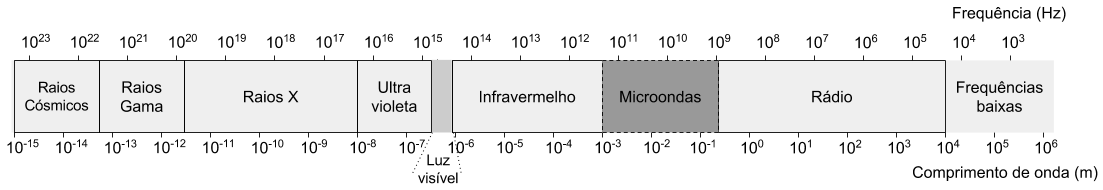
\includegraphics[scale=.4]{figuras/cap3/20EspectroEletromagnetico}
		\caption{\label{fig_20}Espectro Eletromagnético}
	\end{figure}
	
	\par A camada física do padrão WAVE é oriunda de uma transformação da mesma camada no padrão 802.11a. Assim como o 802.11a, o 802.11p utiliza a Multiplexação por Divisão Ortogonal de Frequência (OFDM ou \textit{Orthogonal frequency-division multiplexing}), que comprime os bits contendo os dados em ondas de rádio utilizando-se de técnicas de processamento de sinal. A técnica OFDM divide um largo espectro disponível em vários subcanais de bandas mais estreitas. Cada subcanal é utilizado para carregar parte da informação. As frequências e o tempo de transmissão de cada subcanal são diferentes a fim de que uma transmissão não interfira na outra. 
	
	\par O padrão 802.11p se difere do 802.11a com relação ao ambiente em que vai ser utilizado. O padrão 802.11a é voltado uso em ambientes fechados. pouca mobilidade dos nós e tem alcances curtos. Já a norma 802.11p é voltada para médias distâncias (até 1 quilômetro), alta mobilidade dos nós e mudanças rápidas de canal.
	
	\par Nos Estados Unidos, as redes veiculares foram licenciadas pelo Departamento de Transporte para a operação numa largura de banda de 75MHz, operando na faixa entre 5.850 e 5.925 GHz. Este espectro havia sido separado alguns anos antes para comunicações de alcance curto(DSRC). Por isso, os termos DSRC, WAVE e 802.11p são correlacionados em diversas bibliografias e podem ser usados como sinônimos.
	
	\par Na camada física, a principal emenda acrescida pela norma 802.11p foi operação das interfaces em canais de 10 MHz ao invés de 20 MHz, como eram usados em dispositivos 802.11a. A diminuição da largura do canal foi motivada por estudos feitos por Cheng et al (2008) que demonstraram que os intervalos de guarda em transmissão de 20MHz (0.8$\mu$s) não são suficientemente longos para conter os atrasos gerados por efeitos da propagação multi-percurso, que eram de até 1.5$\mu$s. Um canal de 10MHz tem intervalos de guarda de 1.6$\mu$s. 
	
	\par O espectro que segue na \autoref{fig_21} foi alocado pela Comissão Federal das Comunicações(FCC) dos Estados Unidos para o DSRC. É esperado que os sistemas WAVE desenvolvidos nos EUA trabalhem nos canais definidos pela FCC.
	
	% INSERIR Figura 21 Espectro WAVE - FCC USA
	\begin{figure} [H]
		\centering
		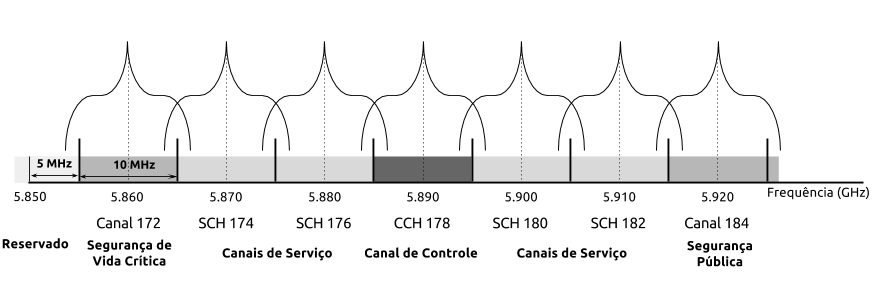
\includegraphics[scale=.5]{figuras/cap3/21EspectroWAVEFCCUSA}
		\caption{\label{fig_21}Espectro WAVE FCC EUA}
	\end{figure}
	
	\par Segundo o padrão 1609.0, o espetro DSRC apresenta as seguintes características no canais:
	
	\begin{itemize}
		\item A faixa de frequência 5850 - 5855 GHz foi colocada em reserva;
		\item O canal 178 é um CCH (\textit{Control Channel} ou Canal de Controle);
		\item Os canais 172, 174, 176, 180, 182 e 184 são SCHs (\textit{Service Channels} ou Canais de Serviço);
		\item Os canais 174 e 176  e os canais 180 e 182 podem ser combinados para produzir 2 canais de 20 MHz, nomeados de canais 175 e 181 respectivamente;
		\item Os canais 172 e 184 são designados a aplicações de segurança pública envolvendo segurança da vida e propriedade. Especificamente alocado pelo FCC nos EUA, o canal 172 é voltado à aplicações de segurança V2V para prevenção e mitigação de acidentes e aplicações para a segurança de vida e de propriedades. O canal 184, por sua vez, se destina à aplicações de mesmo fim atendendo especificamente as comunicações de longa distância e alto consumo. 
	\end{itemize}
	
	\par É importante salientar que o espectro alocado pelo FCC para os EUA pode ou não ser imitado por outros países, como o Brasil. É de escopo da Agência Nacional de Telecomunicações (Anatel) determinar o espectro e a alocação dos canais para os serviços de redes veiculares com fins públicos e privados.
	
	\subsection{Tipos de Canais}
	
	\par Os padrões WAVE especificam duas tipos de canais de rádio. Os dispositivos Car2X que utilizam o padrão WAVE e que têm múltiplas camadas físicas (vários transmissores de rádio) poderão operar um canal de controle (CCH) e pelo menos um canal de serviço(SCH) ao mesmo tempo. Os dispositivos WAVE de apenas um rádio transmissor trabalham alternando entre o canal de controle e os canais de serviço. Para lidar com a limitação de um rádio transmissor, é exigido um sincronismo para que os dispositivos WAVE monitorem cada canal no seu intervalo de tempo específico.
	
	\par O canal de controle é reservado apenas para mensagens do protocolo WSMP e para troca de mensagens de gerenciamento do sistema, como as mensagens de anúncio de serviços WAVE(WSA). As mensagens do protocolo WSMP podem ser recebidas por qualquer dispositivo WAVE com o canal de controle "acordado". Como exemplo, um dispositivo WAVE pode solicitar informações de sincronismo entre rádios por meio de uma requisição broadcast utilizando o protocolo WSMP. O dispositivo WAVE receptor responderia com informações de sincronismo por meio de um quadro de gerenciamento.
	
	\par Os canais de serviço são destinados a operar as transferências de dados de aplicações  diversas, e também podem ser coordenados via mensagens de anúncio de serviço WAVE. Os protocolos WSMP e IPv6 podem ser usados para transmitir informações nos canais de serviço. 
	
	\par Para um melhor entendimento, iremos separar os diferentes tipos serviços WAVE em dois grupos: serviços “anunciados” e serviços “não anunciados”. 
	
	\par Os serviços WAVE “não anunciados” estão geralmente ligados à segurança pública e têm canais fixos. Os serviços “não anunciados” forçam os dispositivos WAVE recebedores a mudar para o canal proposto imediatamente após o envio de uma mensagem de gerenciamento WAVE.
	
	\par Como exemplo, um veículo de segurança pública pode enviar uma mensagem do protocolo WSMP contendo informações de emergência no canal de serviço 172 (canal de segurança pública nos EUA) para que os veículos em seu percurso liberem passagem. Todos os veículos no alcance da unidade de bordo emissora processariam a mensagem imediatamente, propagando a mesma em seguida por meio do canal de serviço 172.
	
	\par Nos serviços "anunciados", um dispositivo WAVE assume o papel de provedor. Este provedor transmite mensagens de anúncio WAVE mediante o canal de controle identificando e descrevendo o serviço e o canal a serem utilizados por este. Os dispositivos WAVE que decidirem se associar ao provedor sintonizam suas antenas no canal proposto pela WSA, se tornando usuários deste provedor. Assim feito, o  dispositivo provedor e os usuários poderão trocar informações associadas com o serviço oferecido. 
	
	\par Como exemplo, a \autoref{fig_22} representa um cenário no qual há 3 unidades de acostamento, todas instaladas em postes de iluminação ao longo da rodovia. Neste cenário, cada unidade de acostamento está transmitindo anúncios de serviço WAVE via canal de controle contendo a Identificação do Serviço com o valor 0x04, atribuído ao serviço de aconselhamento de tráfego para viajantes. As unidades de acostamento enviam as mensagens de anúncio (WSAs) na forma de broadcast contendo avisos sobre o tráfego local em um canal proposto e respondem a requisições para informações adicionais de tráfego usando IPv6. Quando os dispositivos usuários entrarem na área de cobertura das unidades de acostamento, estes irão receber as WSAs e avaliarão se o valor da identificação de serviço é desejado. Os dispositivos usuários que têm interesse em aconselhamento de tráfego (neste cenário representados pelo caminhão verde e pelo carro vermelho) aceitarão este serviço e sintonizarão no canal especificado. Os dispositivos usuários que não têm interesse neste serviço irão simplesmente descartar os pacotes recebidos.
	
	%INSERIR Figura 22 Tipos de Canais - SCH
	\begin{figure} [H]
		\centering
		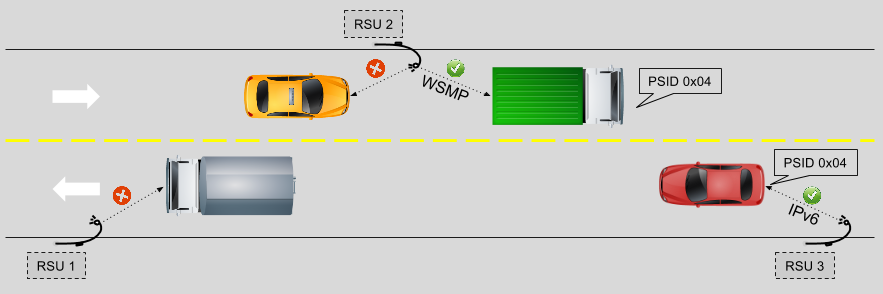
\includegraphics[scale=.5]{figuras/cap3/22TiposDeCanais}
		\caption{\label{fig_22}Tipos de Canais}
	\end{figure}
	
	\section{Subcamada MAC}
	
	\par Na camada de enlace também foram acrescidas emendas, sobretudo na subcamada MAC. Diferentemente de uma conexão sem fio tradicional, na qual o MAC do \textit{Access Point} está presente no cabeçalho do \textit{frame}, a norma 802.11p define um método de troca de informações mais rápido, sem o estabelecimento de um BSSID real. Um BSSID “coringa” (com os valores binários em 1’s) é utilizado no cabeçalho dos \textit{frames} trocados. Este é inserido no campo Endereço 3 do cabeçalho MAC (\autoref{fig_23}). 
	
	%INSERIR Figura 23 Cabeçalho 802.11 MAC E 802.11p WAVE
	\begin{figure} [H]
		\centering
		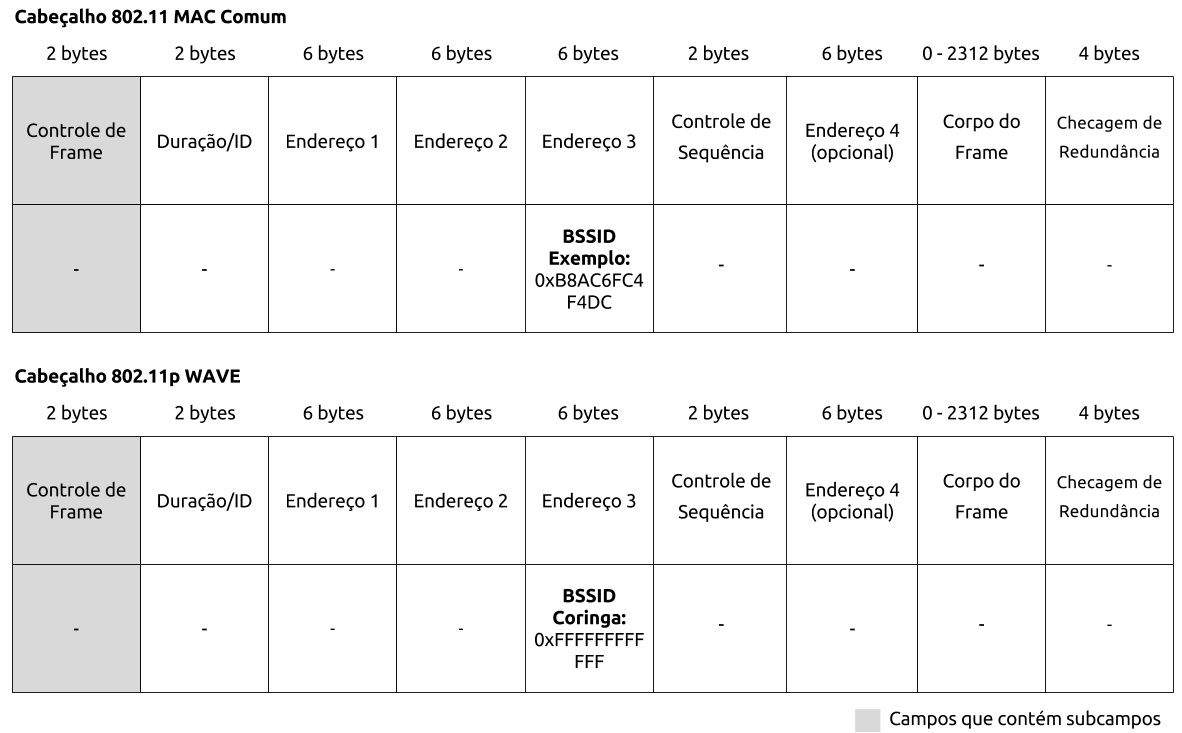
\includegraphics[scale=.38]{figuras/cap3/23ExemploMACComumMACWAVE}
		\caption{\label{fig_23}Exemplo de MAC Comum e MAC WAVE}
	\end{figure}

	
	\par Além disso, a emenda adiciona à MIB (Ver mais em \autoref{MIB}) do protocolo de gerenciamento SNMP a variável \textbf{dot11OCBActivated} como booleana. OCB (\textit{On the Context of} BSS) significa no contexto do BSS. Caso for configurada como verdadeira e o BSSID Coringa for utilizado, a conexão entre os pares é realizada dispensando os procedimentos de associação, autenticação e confidencialidade de dados. Estes serviços então seriam de responsabilidade das camadas superiores.
	
	\par Também foi adicionado por intermédio da emenda 802.11p um quadro de gerenciamento para anúncio de hora a fim de que as estações 802.11p sincronizem entre si uma referência de hora comum. A única referência definida na emenda é o padrão UTC (\textit{Universal Time Coordinated} ou Tempo Universal Coordenado).
	
	\subsection{Operações multi-canal}
	
	\par Os dispositivos WAVE implementam operações e serviços que suportam conectividade multi-canal na subcamada de acesso ao meio (MAC), baseando-se na norma IEEE 1609.4. Esta norma descreve mecanismos efetivos que controlam a transferências de dados de camadas superiores através de múltiplos canais. Outra norma descrita nesta seção é a IEEE 802.11 MAC, que trata de forma mais abrangente a coordenação de múltiplos canais em redes sem fio.
	
	\par Conforme visto na \autoref{fig_18}, o padrão WAVE tem uma pilha contendo protocolos, entidades de gerenciamento e serviços de segurança. As entidades de gerenciamento são importantes para o funcionamento dos protocolos pois proveêm as interfaces de serviços por meio das quais as funções de gerenciamento de cada camada podem ser chamadas.
	
	\par O padrão IEEE 1609.4 adiciona extensões ao modelo de subcamada MAC do padrão 802.11 para adaptação ao meio veicular. Para realizar operações sobre múltiplos canais sem fio tendo o parâmetro \textit{OCBActivated} como verdadeiro, há necessidade de realizar a coordenação de canal, o que é proposto no padrão mencionado.
	
	\par Na subcamada MAC, a entidade MLME (mostrada na \autoref{fig_19}) é responsável por gerenciar os serviços de coordenação do canal e por auxiliar a entrega das unidades de dados de serviço MAC.
	
	\subsection{Serviços do Plano de Dados} 
	\label{subsec:Serviços do Plano de Dados}
	
	\par Os serviços executados pela MLME são inerentes ao Plano de Dados e ao Plano de Gerenciamento. Os serviços MLME no Plano de Dados abrangem:
	
	\begin{description}
        \item[Coordenação de canal]
    \end{description}
	
	\par A coordenação de canal pela subcamada MAC garante que os pacotes serão transmitidos no canal sem fio pretendido e permite a troca de dados entre dispositivos com operações alternadas e concorrentes em múltiplos canais. Esta última característica permite que dispositivos WAVE com uma única camada física utilizem o acesso alternado na coordenação de canal. Como exemplo, num dispositivo WAVE de única camada física os tráfegos de alta prioridade e de gerenciamento operariam no canal de controle em intervalo de tempo 0 enquanto o tráfego geral de camadas superiores atuaria no canal de serviço durante intervalo de tempo 1. 
	
	\par Os dispositivos WAVE de várias camadas físicas podem utilizar o acesso contínuo na utilização de canal de controle ou canal de serviço, sem necessitar de alguma coordenação. Também é possível que haja acesso alternado entre os canais de serviço. A coordenação de canais é mostrada na \autoref{fig_24}.
	
	\begin{description}
        \item Exemplos:
    \end{description}
    
	\begin{description}
		\item[(A)] Um dispositivo WAVE A pode acessar o canal de controle em intervalo de tempo 0 e um canal de serviço em intervalo de tempo 1;
		\item[(B)] Um dispositivo WAVE B pode acessar um canal de serviço em intervalo de tempo 0 e o canal de controle em intervalo de tempo 1;
		\item[(C)] Este mesmo dispositivo WAVE B em algum tempo depois pode acessar um canal de serviço em intervalo de tempo 0 e outro canal de serviço em intervalo de tempo 1.	
	\end{description}
	
	%INSERIR Figura 24 Exemplos de acesso ao canal
	\begin{figure} [H]
		\centering
		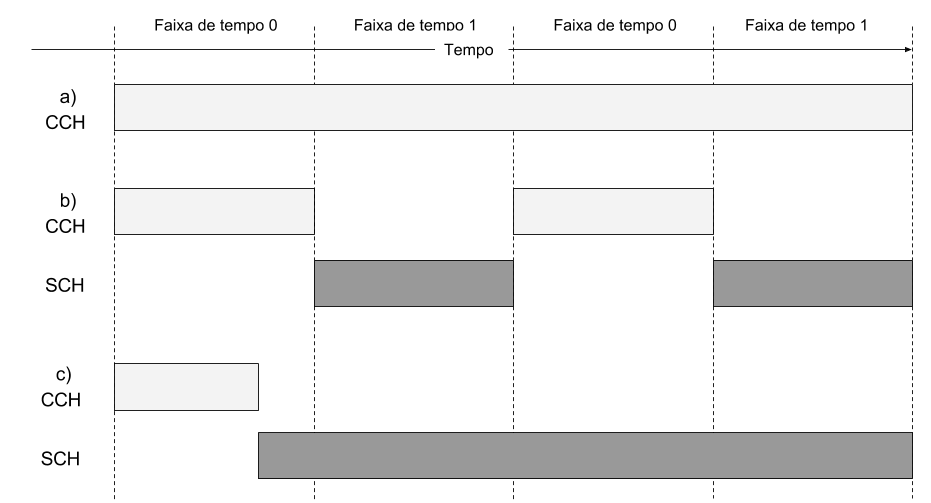
\includegraphics[scale=.5]{figuras/cap3/24ExemplosDeAcessoAoCanal}
		\caption{\label{fig_24}Exemplos de Acesso ao Canal}
	\end{figure}
	
	\par Esta alternação entre o CCH e SCH depende de um mecanismo de sincronização entre os dispositivos participantes, que é garantido pelo Serviço de Gerenciamento Sincronização multi-canal. Também é definido um período de guarda no início de cada intervalo de tempo com o objetivo de compensar os efeitos de comutação de rádio e imprecisões no sincronismo, como mostrado na \autoref{fig_25}.
	
	%INSERIR Figura 25 Intervalo de sincronismo e de guarda
	\begin{figure} [H]
		\centering
		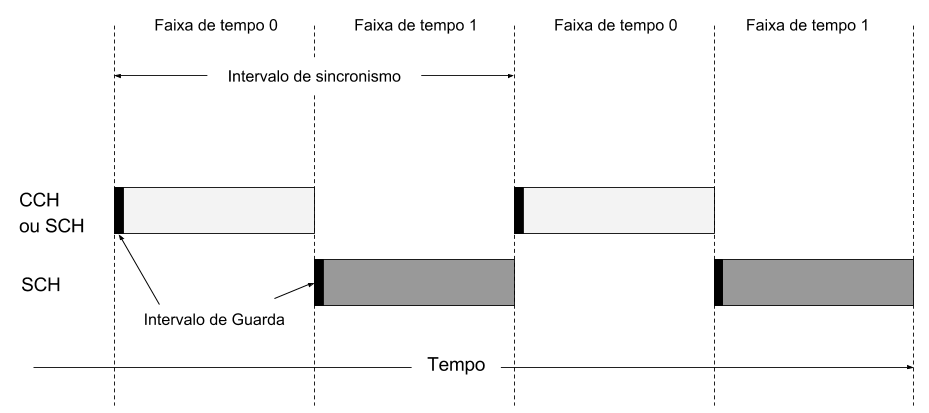
\includegraphics[scale=.5]{figuras/cap3/25IntervaloDeSincronismoEDeGuarda}
		\caption{\label{fig_25}Intervalo de Sincronismo e de Guarda}
	\end{figure}
	
	\begin{description}
        \item[Roteamento de canal]
    \end{description}
	
	\par A subcamada MAC lida com dados de entrada e saída das camadas superiores, roteando os pacotes de dados de uma camada superior até o canal designado e configurando os parâmetros para transmissões sem fio WAVE. Do lado do destinatário, a subcamada MAC garante o roteamento de pacotes para o protocolo de camada superior correto.
	
	\par O protocolo WSMP define o canal, a potência de transmissão e a taxa de transferência a cada mensagem. Quando dados WSMP são recebidos na subcamada MAC, os pacotes são direcionados à filas para a transmissão de acordo com o \textbf{identificador do canal} e a \textbf{prioridade}. Logo após, a subcamada MAC deve transmitir o pacote dentro do intervalo de tempo indicado, com taxa de transferência e potência de transmissão determinadas.
	
	\par Datagramas IP, entretanto, têm os parâmetros canal, potência de transmissão e taxa de transferência armazenados no perfil do transmissor. Os pacotes IP são recebidos pela subcamada MAC e colocados em filas de acordo com o nível de prioridade para a transmissão no SCH. Utilizando os parâmetros estabelecidos no perfil do transmissor, os pacotes são enviados por meio da camada física caso a MLME delibere acesso.

	\newpage
	
	\begin{description}
        \item[Prioridades de pacotes]
    \end{description}

	% INSERIR Figura 26 MAC (Multi-Canal)
	\begin{figure} [H]
		\centering
		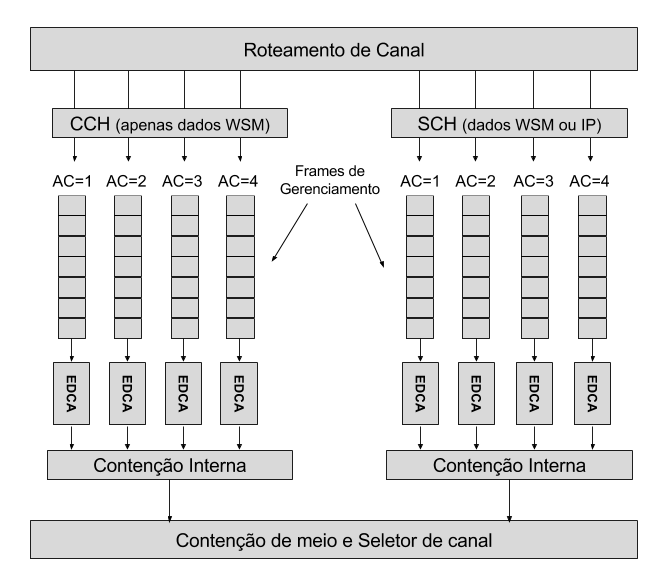
\includegraphics[scale=.5]{figuras/cap3/26MAC(MultiCanal)}
		\caption{\label{fig_26}MAC(Multi-Canal)}
	\end{figure}
	
	\par Os padrões WAVE suportam Qualidade de Serviço (\textit{Quality of Service} ou QoS) nos pacotes aplicando as técnicas EDCA (\textit{Enhanced Distributed Channel Access} ou Acesso ao Canal Distribuído Aprimorado).
	
	\par Quando um pacote WSMP ou IPv6 chega na subcamada MAC, tendo o roteamento do canal apropriadamente finalizado, esta deverá “enfileirar” os dados de acordo com a categoria de acesso indicada (valores entre 1 e 4). A \autoref{fig_26} ilustra as filas e o roteamento do canal. O mapeamento dos pacotes atribuindo o indicador de prioridade é tratado pelo padrão IEEE 802.11. Os Provedores de Serviço WAVE podem opcionalmente anunciar parâmetros EDCA via anúncio de serviço WAVE. Caso nenhum parâmetro EDCA seja especificado, o EDCA padrão é ativado.
	
	\subsection{Serviços do Plano de Gerenciamento}
	
	\par Em adição aos serviços de gerenciamento MLME mencionados no padrão 802.11 para redes sem fio em geral, o padrão WAVE IEEE 1609.4 adiciona características de acesso ao canal e sincronização de dispostivos WAVE em apoio à coordenação de canal, manutenção da MIB e reendereçamento.
		
	\newpage
	
	\begin{description}
        \item[Sincronização multi-canal]
    \end{description} 
	
	\par A entidade da subcamada MAC(MLME) utiliza uma base de tempo comum que pode ser obtida localmente ou recebida via rádio para gerar uma função de sincronismo com objetivo de alinhar os intervalos de tempo entre os dispositivos WAVE comunicantes. A MLME gera quadros de anúncio de sincronismo para distribuição de informação de sincronismo e monitora os estes quadros recebidos.
	
	\par A referência de tempo comum usada para o sincronismo multi-canal é o módulo 1 segundo da UTC, utilizado por muitos equipamentos GPS.
	
	\par Parâmetros como intervalo de guarda, tolerância de sincronização e tempo máximo de troca de canal são gerenciados pelo Serviço de Gerenciamento de Sincronização Multi-canal.
	
	
	\begin{description}
        \item[Acesso ao canal]
    \end{description}
	
	\par A MLME controla o acesso aos canais de rádio específicos em suporte às requisições recebidas da entidade de gerenciamento WAVE (WME ou WAVE \textit{Manager Entity}). Opções de acesso a canal incluem acesso contínuo, acesso alternado e acesso imediato, evidenciado pela \autoref{fig_24}.
	
	\begin{description}
		
		\item[(A)] Acesso contínuo: o canal designado fica disponível por duração indefinida;
		\begin{itemize}
			\item Um dispositivo WAVE configurado para operar em um único canal de serviço ou de controle.
		\end{itemize}
		
		\item[(B)] Acesso alternado: o acesso é alternado entre os canais de serviço ou entre o canal de controle e um canal de serviço;
		\begin{itemize}
			\item Um dispositivo WAVE configurado para monitorar anúncios de serviço no canal de controle. Quando o canal de controle recebe um anúncio de serviço WAVE de seu interesse, o dispositivo o alterna para o canal de serviço durante do intervalo de tempo 1 para participar da aplicação de interesse, retornando ao canal de controle durante intervalo de tempo 0 para monitoramento de outras WSAs ou qualquer outra atividade. Alternativamente, um dispositivo pode ser configurado para alternar entre canais de serviço também.
		\end{itemize}
		
		\item[(C)] Acesso imeditado: o acesso é mudado por tempo determinado ou indefinido;
		\begin{itemize}
			\item Um dispositivo é configurado para monitorar um canal de controle. Ao receber uma WSA com uma aplicação de interesse, o dispositivo alterna imediatamente para um canal de serviço por um tempo específico a fim de completar determinada atividade. Ao término desta atividade, o dispositivo retorna ao primeiro canal.
		\end{itemize}		
	\end{description}
	
	\begin{description}
        \item[Outros serviços IEEE 802.11]
    \end{description}
	
	\par A MLME permite outros serviços 802.11 que podem ser chamados por cada canal independentemente.
	
	\begin{description}
        \item[Manutenção da Base de Gerenciamento de Informação (MIB)]
    \end{description}
	
	\par A MLME mantém uma Base de Gerenciamento de Informação contendo informações de configuração e status.
	
	\begin{description}
        \item[Reendereçamento]
    \end{description}
	
	\par A MLME permite alterações dinâmicas no endereço MAC a fim de suportar pseudonimato. O pseudonimato é uma propriedade  em que identidades e padrões de comportamento de entidades não podem ser deduzidos pelo tráfego de rede, sendo apenas observáveis por partes propriamente autorizadas.
	
	\section{\label{sec:llc}Subcamada LLC}
	
	\par Definida no padrão 1609.3, a subcamada de Controle de Enlace Lógico do modelo WAVE está imediatamente acima da subcamada MAC. A subcamada LLC do modelo WAVE é parte essencial no direcionamento dos dados para processamento nas camadas superiores. 
	
	\par Nesta camada, é utilizado o protocolo SNAP. No cabeçalho deste protocolo há o campo \textit{Type} que revela o valor \textit{Ethertype}. Este valor indica qual protocolo da camada imediatamente acima será introduzido. A \autoref{fig_27} mostra o cabeçalho do protocolo SNAP juntamente ao cabeçalho LLC em mais detalhes.
	
	%INSERIR Figura 27 Cabeçalho LLC
	\begin{figure} [H]
		\centering
		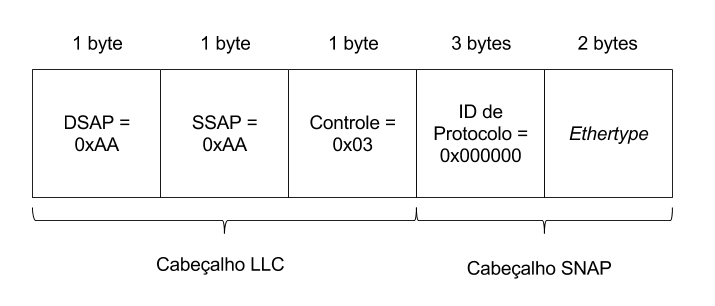
\includegraphics[scale=.5]{figuras/cap3/27CabecalhoLLC}
		\caption{\label{fig_27}Cabeçalho LLC}
	\end{figure}
	
	\par Iniciando pelo cabeçalho do LLC, os campos de 1 byte DSAP e SSAP são sempre configurados com o dígitos hexadecimais 0xAA (valor binário 10101010) indicando encapsulamento.
	
	\par O campo de 1 byte \textbf{control} é utilizado para verificar se os dados são sequenciais ou não. São sempre configurados com os dígitos hexadecimais 0x03 (valor binário 00000011) indicando o uso de transporte de dados sem conexão e que os dados não precisam ser sequenciados ou reconhecidos.
	
	\par No cabeçalho do protocolo SNAP, o campo \textbf{Protocol ID} ou também chamado de OUI (\textit{Organization Unique Identifier}) tem tamanho de 3 bytes e é configurado com os dígitos hexadecimais 0x000000 indicando que o protocolo a ser utilizado na camada acima é do tipo \textit{Ethernet} (\textbf{Ethertype}).
	
	\par O campo \textbf{Type} é o campo que indica qual protocolo será utilizado na camada imediatamente acima, isto é, a camada de rede. O tamanho do campo é de 2 bytes. No caso dos padrões WAVE, apenas dois protocolos são possíveis na camada de rede: IPv6 ou WSMP. 
	
	\par O processamento da transmissão de um pacote da camada de rede funciona da seguinte maneira: 
	
	\par O protocolo da camada de rede requisita a transmissão de um pacote e a subcamada LLC configura o campo \textbf{Type} ao valor \textit{Ethertype} correspondente. 
	
	\begin{itemize} %[?] FICA ASSIM MSM?
	    \item Se o protocolo a ser chamado for o WSMP, uma primitiva chamada DL-UNITDATAX.request é acionada e o valor \textit{Ethertype} atribuído no campo Type é 0x88DC. Os dados são transmitidos para as camadas inferiores usando a primitiva MA-UNITDATAX.request. 
        \item Se o protocolo for o IPv6, uma primitiva chamada DL-UNITDATA.request é acionada e o valor \textit{Ethertype} atribuído no campo Type é 0x86DD. Os dados são transmitidos para as camadas inferiores usando a primitiva MA-UNITDATA.request.
    \end{itemize}
	
	\par O processamento de recebimento de um pacote na subcamada LLC funciona da seguinte maneira: 
	\begin{enumerate}
		\item A subcamada MAC envia um quadro via primitiva MA-UNITDATA.indication.
		\item A subcamada LLC lê o campo Type contendo o valor \textit{Ethertype} e extrai o pacote.
		\begin{description}
			\item[A.] Se o valor no campo Type é 0x88DC, a subcamada LLC entrega o pacote para WSMP.
			\item[B.] Se o valor no campo Type é 0X86DD, a subcamada LLC entrega o pacote para IPv6.
		\end{description}
		\item Em ambos protocolos, o pacote é entregue da subcamada LLC para as camadas superiores via primitiva DL-UNITDATA.indication.	
	\end{enumerate}
	
	\section{Camadas de Rede e Transporte}
	
	\par Como as camadas de rede e transporte no modelo WAVE estão intrinsicamente relacionadas, especialmente no protocolo WSMP, estas serão discutidas em seção única.
	
	\par Os protocolos da camadas de Rede e Transporte WAVE são definidos em grande parte no padrão IEEE 1609.3 - Serviços de Rede. Este padrão especifica duas pilhas de protocolos na camada de rede (\autoref{fig_17}), IPv6 e WSMP. Esta pilha de protocolos distingue-se entre as duas camadas superiores no campo \textit{Ethertype} conforme explicado na \autoref{sec:llc}.
	
	\par O protocolo WSMP foi projetado para otimizar operações em Redes Veiculares, sendo indicado para serviços que necessitam de troca rápida de mensagens. Também é possível a utilização de tráfego IP para serviços que necessitam de conexão com a Internet para obtenção de dados na nuvem. O protocolo IPv6 gera um volume superior de tráfego na rede, sendo apenas permitido nos canais de serviço para não comprometer a performance do WSMP nos canais de controle.
	
	\subsection{Protocolo WSMP}
	
	\par A família de padrões WAVE é constituida por uma pilha de protocolos de comunicação otimizada para o ambiente veicular, provendo protocolos da camada de rede e transporte. O protocolo WSMP consiste de uma camada de serviços de rede, uma camada de transporte e uma entidade associada do plano de gerenciamento, a entidade de gerenciamento WAVE (WME ou WAVE Management Entity). O escopo do protocolo WSMP nesta seção é mostrado na \autoref{fig_28}.
	
	%INSERIR Figura 28 Escopo do Tópico
	\begin{figure} [H]
		\centering
		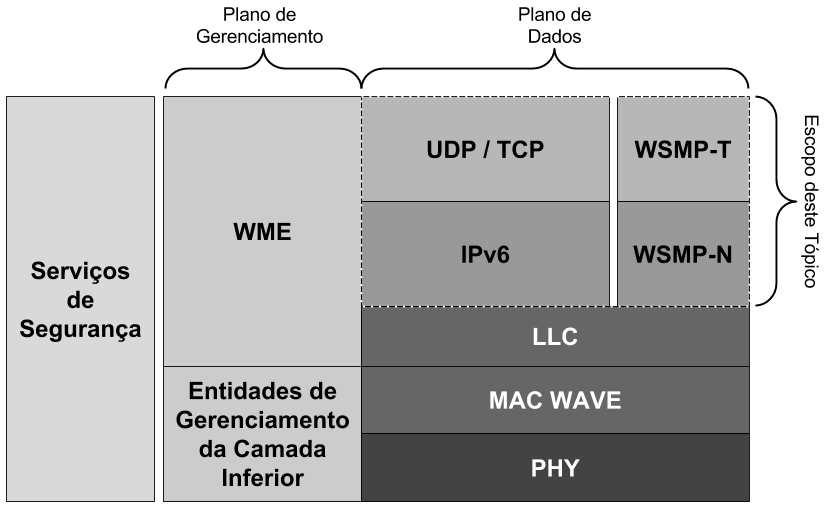
\includegraphics[scale=.45]{figuras/cap3/28Escopo}
		\caption{\label{fig_28}Escopo do WSMP nesta seção}
	\end{figure}
	
	\par Nas redes sem fio tradicionais, as aplicações estão preocupadas em apenas enviar e receber informações. Desta forma, detalhes da camada física como canal de transmissão e potência do sinal não são definidos pelas aplicações.
	
	\par No padrão WAVE, o protocolo WSMP permite que aplicações controlem diretamente as características da camada física (como o canal ou potência do transmissor) a serem utilizadas na transmissão das mensagens. A aplicação de origem também provê um identificador do Provedor de Serviço (PSID ou (\textit{Provider Service Identifier}), que é utilizado como um direcionador da  aplicação no receptor, além de marcar o endereço MAC do dispositivo de destino com a possibilidade de um endereço de grupo para \textit{multicast} ou broadcast.
	
	\par As mensagens curtas WAVE (WSMs ou WAVE \textit{Short Messages}) são entregues para a entidade de destino correta baseados no PSID. Caso o valor do PSID no cabeçalho de uma mensagem recebida representar um serviço que não seja de interesse local, a mensagem pode ser ignorada. Os procedimentos de aceitação de uma mensagem curta WAVE por meio do PSID serão explicados em maior detalhe na \autoref{subsubsec:TransRecWSM}.

	\subsubsection{\label{sssec:wsm}Mensagem Curta WAVE}
	
	\par  Quando a camada de aplicação requisita o envio de uma mensagem, esta é encapsulada dentro do campo \textbf{dados WSM} de uma mensagem curta WAVE (WSM). Mensagens Curtas WAVE são formadas pelo \textbf{cabeçalho} do protocolo WSMP em conjunto com os \textbf{dados da WSM}.
	
	\par A \autoref{fig_29} ilustra como este cabeçalho é construído conforme os dados são movidos da camada de aplicação através dos Serviços de Rede{\footnote{\textbf{Serviços de Rede} comprime os serviços da Camada 3 (Rede) e Camada 4 (Transporte) do Modelo OSI conforme pode ser visto na \autoref{fig_28}.}} até a camada MAC. As caixas com borda pontilhada são opcionais e não fazem parte do pacote em si, mas podem ser enviadas para as camadas inferiores como parâmetros por meio das primitivas ("funções" em itálico na \autoref{fig_29}). As caixas com borda preenchida indicam  os campos formatados para a transmissão.

	%INSERIR Figura 29 Composição de uma WSM
	\begin{figure} [H]
		\centering
		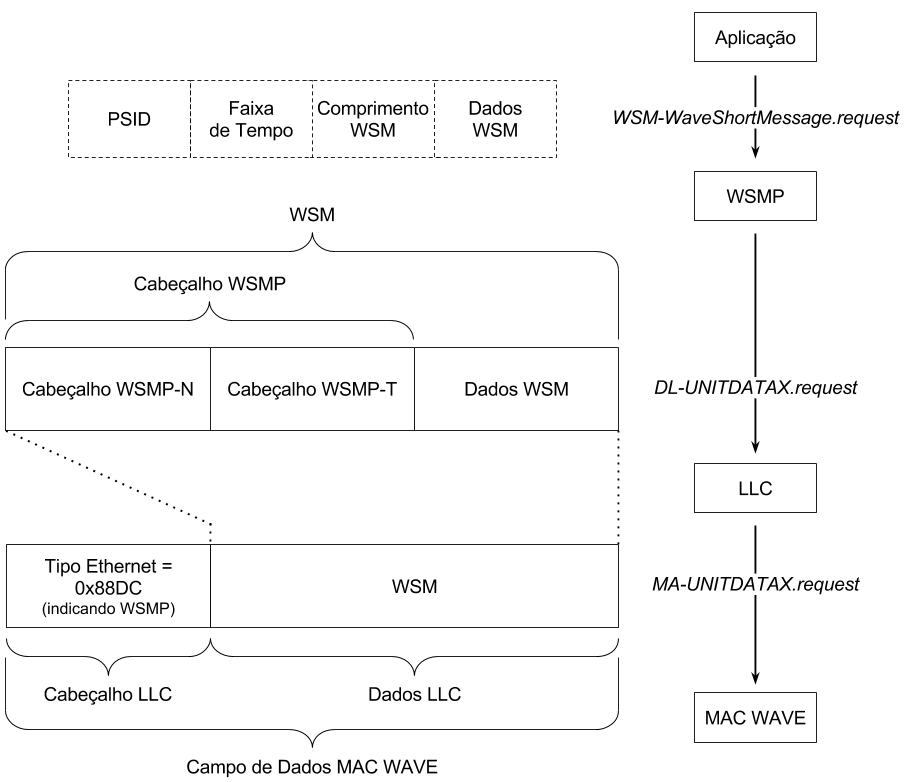
\includegraphics[scale=.5]{figuras/cap3/29ComposicaoDeUmaWSM}
		\caption{\label{fig_29}Composição de uma WSM}
	\end{figure}
	
	\par Conforme mostra a \autoref{fig_29}, o cabeçalho do protocolo WSMP-N (camada de rede do protocolo WSMP) é composto por um campo \textbf{subtipo} de 4 bits, um \textbf{indicador de campos opcionais WSMP-N} de 1 bit, um campo de \textbf{versão do WSMP} de 3 bits, e um campo de identificação para o protocolo de transporte (\textbf{TPID}) de 8 bits. Existe também o campo opcional chamado de \textbf{informações extensíveis do elemento WAVE}.
	
	%INSERIR Figura 30 Composição de uma WSM
	\begin{figure} [H]
		\centering
		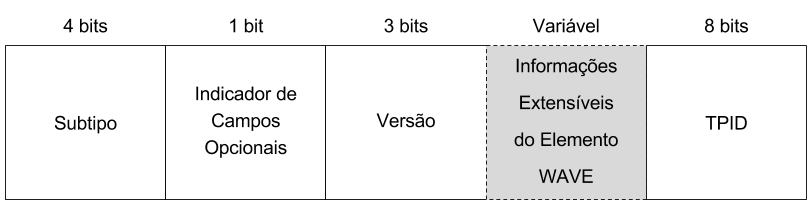
\includegraphics[scale=.5]{figuras/cap3/30CabecalhoDeRedeWSMPPadrao(Subtipo0)}
		\caption{\label{fig_30}Cabeçalho de Rede WSMP Padrão(Subtipo = 0)}
	\end{figure}
	
	\par O suporte para o campo \textbf{subtipo} com valor 0 (Protocolo de Redes Nulo) é obrigatório. Já o suporte para outros valores de subtipos são possíveis mas não foram descritos no padrão IEEE 1609.3.
	
	\par O campo \textbf{indicador de campos opcionais WSMP-N} contendo valor 1 aponta a presença de \textbf{informações extensíveis do elemento WAVE}. Caso o valor seja 0, o campo extensível deve ser desconsiderado. Informações adicionais sobre os campos extensíveis WAVE podem ser encontradas no \autoref{att:InfoElemWAVE}).
	
	\par O campo \textbf{versão do WSMP} indica qual versão do protocolo WSMP é utilizada. Mensagens curtas WAVE com diferentes valores de versão indicam incompatibilidade entre o formato e o emprego das mensagens. Caso um dispositivo WAVE receba uma mensagem curta com o um valor de  versão não suportado, este não processará a mensagem. 
	
	\par O campo \textbf{TPID} recebe valores entre 0 e 255. Este campo indica a característica do protocolo de transporte a ser utilizada e especifica qual será a estrutura do cabeçalho de transporte WSMP (\textbf{WSMP-T}).
	
	%INSERIR Figura 31 Cabeçalho de Transporte WSMP Padrão
	\begin{figure} [H]
		\centering
		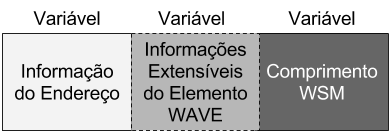
\includegraphics[scale=.6]{figuras/cap3/31CabecalhoDeTransporteWSMPPadrao}
		\caption{\label{fig_31}Cabeçalho de Transporte WSMP Padrão}
	\end{figure}
	
	\par A \autoref{fig_31} demonstra um cabeçalho \textbf{WSMP-T} genérico. O conteúdo do campo \textbf{informação do endereço} depende do valor do \textbf{TPID} inserido. A presença dos campos de \textbf{informações extensíveis do elemento WAVE} também depende do \textbf{TPID}. O campo \textbf{comprimento WSM} é obrigatório e indica o tamanho do campo \textbf{dados WSM}.
	
	\par A \autoref{fig_32} apresenta os diferentes formatos do cabeçalho de transporte WSMP (\textbf{WSMP-T}). Para valores de \textbf{TPIDs} iguais a 1 ou 3, o campo \textbf{informações extensíveis do elemento WAVE} estará presente, enquanto nos valores 0 ou 2 não. O \textbf{comprimento WSM} sempre estará presente. O campo \textbf{informação do endereço} também muda de acordo com o \textbf{TPID}.
	
	\par O suporte para \textbf{TPID} 0 e 1 são obrigatórios. Os demais \textbf{TPIDs} não são especificados pelo padrão IEEE 1609.3.
	
	\par Para \textbf{TPIDs} com valores iguais a 0 ou 1, a \textbf{informação do endereço} é composta apenas do \textbf{PSID}. O \textbf{PSID} é o endereço de destino que indica qual camada de aplicação deve receber a mensagem. O endereço de origem não é conhecido.
	
	\par Para \textbf{TPIDs} com valores iguais a 2 ou 3, a \textbf{informação do endereço} é composta pelos valores das portas de origem e de destino dos dispositivos WAVE. 
	
	%INSERIR Figura 32 Diferentes formatos do Cabeçalho WSMP-T de acordo com TPID
	\begin{figure} [H]
		\centering
		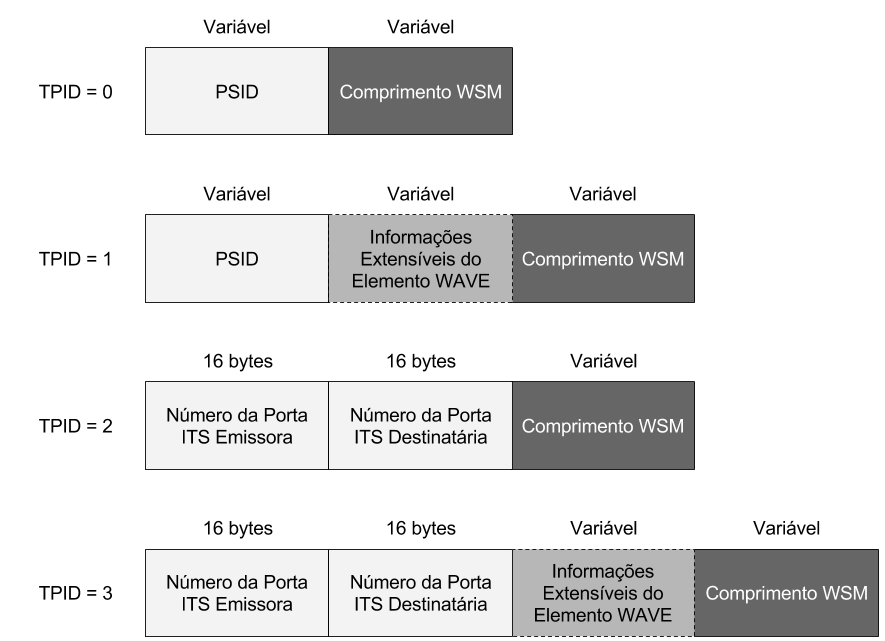
\includegraphics[scale=.45]{figuras/cap3/32DiferentesFormatosTPID}
		\caption{\label{fig_32}Diferentes formatos do Cabeçalho WSMP-T de acordo com TPID}
	\end{figure}

	\subsubsection{Mensagem de Anúncio WAVE}
	
	\par Um anúncio de serviço WAVE (WSA) é a compressão das informações de um serviço na forma de mensagens. Conforme a \autoref{fig_33}, uma WSA formatada (denominada \textit{Ieee1609Dot2Data} pelo padrão WAVE) é inserida no campo \textbf{dados WSM} e enviada pelo dispositivo WAVE com o valor do \textbf{PSID} 0x87, atribuído para anúncios de serviços WAVE.
	
	\par Esta mensagem formatada poderá ser uma WSA segura ou não segura.
		
	%INSERIR Figura 33 Modelos de uma WSA
	\begin{figure} [H]
		\centering
		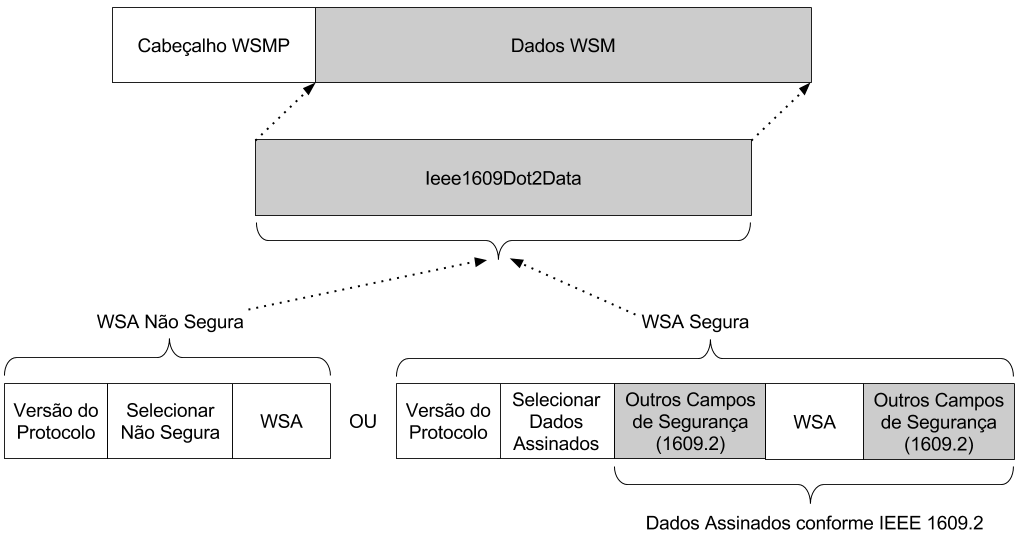
\includegraphics[scale=.4]{figuras/cap3/33ModelosWSA}
		\caption{\label{fig_33}Modelos de uma WSA}
	\end{figure}
	
	\par Não há nenhuma especificação para mensagens WSA não seguras, enquanto WSA seguras podem atender a duas especificações diferentes: mensagens assinadas ou mensagens encriptadas.
	
	\par O padrão IEEE 1609.11 propõe uma aplicação de coleta eletrônica de taxas, onde as trocas de informações para o pagamento de pedágios devem ser encriptadas com intuito de garantir a privacidade dos dados do cartão do motorista. Já mensagens assinadas são utilizadas para garantir que determinado serviço anunciado pertença a um provedor confiável. Conforme proposto por Whyte et al(2015) toda anúncio de serviço WAVE deveria ser assinado, garantindo que punições sejam aplicadas aos provedores que divulgam WSAs maliciosas.
	
	\par Mensagens assinadas podem contemplar os serviços de: autenticidade, indicando que a mensagem realmente foi enviada pela origem indicada; autorização, assegurando que o dispositivo de origem tem acesso aos privilégios requisitados; e integridade, certificando que qualquer mudança na mensagem será detectável. Mensagens Encriptadas devem ser confidenciais, garantindo que apenas os dispositivos determinados terão acesso ao conteúdo da mensagem.
	
	\par É possível configurar os dispositivos WAVE para receberem apenas anúncios de serviços assinados, de forma similar ao que acontece com a escolha de \textbf{PSIDs} aceitos pelo dispositivo.
	
	%INSERIR Figura 34 Cabeçalho WSA
	\begin{figure} [H]
		\centering
		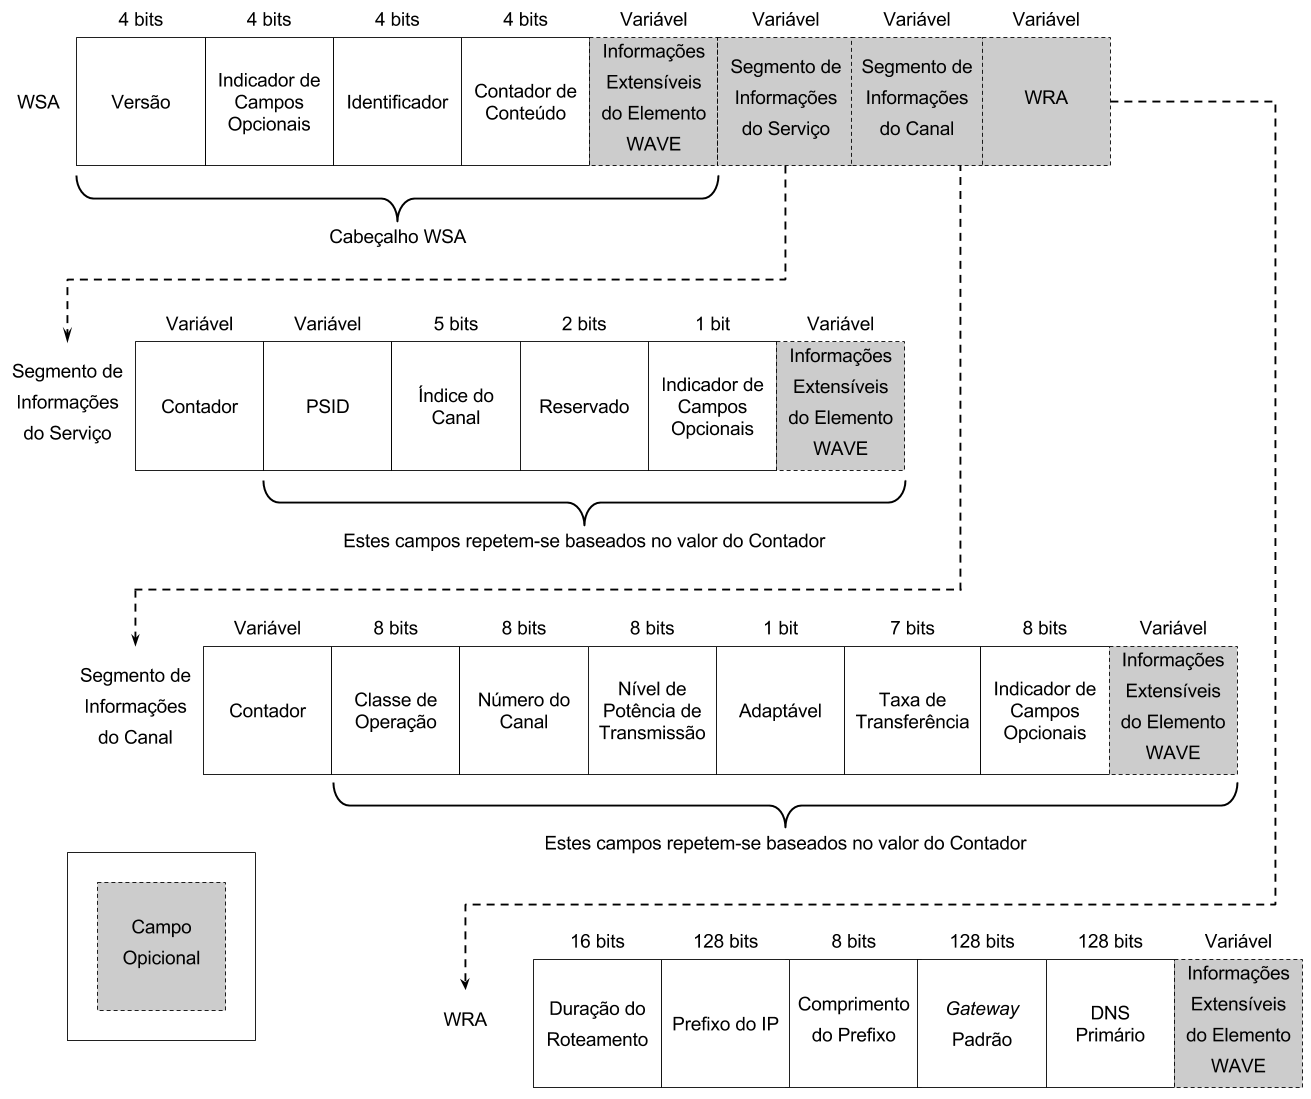
\includegraphics[scale=.3]{figuras/cap3/34CabecalhoWSA}
		\caption{\label{fig_34}Cabeçalho de WSA}
	\end{figure}
	
	\par A \autoref{fig_34} exibe o cabeçalho de uma anúncio de serviço WAVE. Pode-se perceber a existência de diversos campos, entretanto, não é de escopo deste trabalho entrar em detalhes nos informações que compõe uma WSA.
	
	\subsubsection{Transmissão e recepção de mensagens curtas WAVE}
	\label{subsubsec:TransRecWSM}

	\par Visando uma melhor compreensão da transmissão e recepção de uma mensagem curta WAVE, considere o seguinte exemplo de uma troca de WSMs. Uma aplicação de origem prepara os dados da mensagem para transmissão e seleciona um endereço MAC de broadcast. Baseado nas configurações especificadas para esta mensagem, a aplicação informa as configurações da camada física (potência de transmissão, taxa de transferência) e invoca a primitiva de requisição de mensagem curta WAVE (WSM-WaveShortMessage.request) para solicitar que o protocolo WSMP entregue o pacote resultante para as camadas inferiores com o intuito de serem transmitidas no canal selecionado.

	\par É possível perceber no exemplo que o canal, a faixa de tempo, a potência de transmissão, a taxa de transferência e o canal podem ser definidos conforme o envio de mensagens são requisitados.	
	
	\par O protocolo WSMP provê funções da camada de rede por meio do seu cabeçalho de rede (\textbf{WSMP-N}). Este protocolo também fornece funções da camada de transporte por intermédio do cabeçalho de transporte (\textbf{WSMP-T}). Diferentes primitivas são utilizadas para a troca de informação entre os componentes conforme apresentado na \autoref{fig_37}.
	
	%INSERIR Figura 37 Transmissão e Recepção de uma WSM
	\begin{figure} [H]
		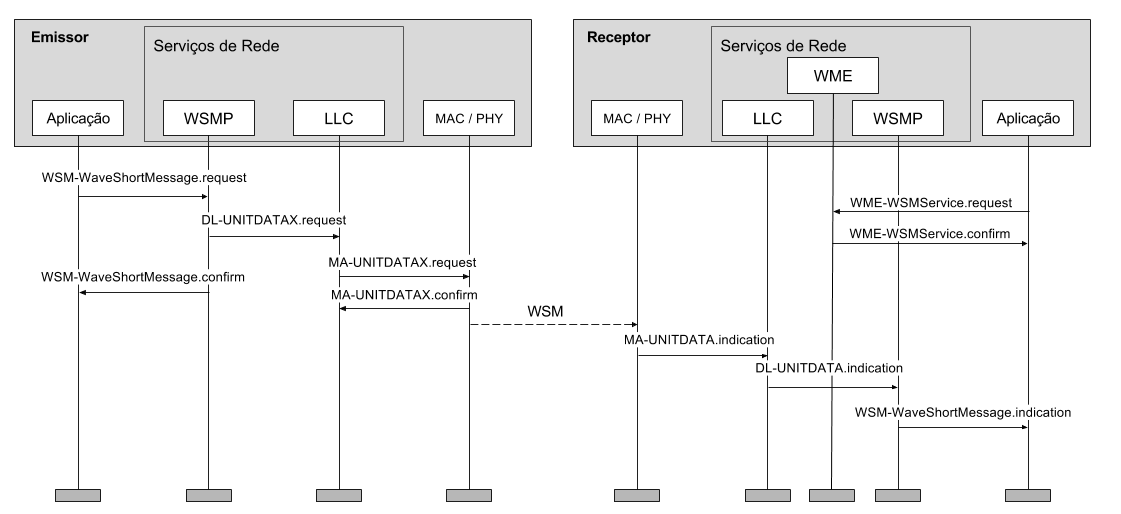
\includegraphics[scale=.4]{figuras/cap3/37TransmissaoRecepcaoWSM}
		\caption{\label{fig_37}Transmissão e Recepção de uma WSM}
	\end{figure}

	\par Ao receber uma \textit{WSM-WaveShortMessage.request} de uma aplicação, a protocolo WSMP{\footnote{Serviços de Rede e Transporte vide \autoref{fig_28}}} verifica se o comprimento do cabeçalho está de acordo com o limite proposto pelo \textit{WsmMaxLength} da MIB da entidade de gerenciamento WAVE. Caso a verificação seja positiva, o cabeçalho WSMP é gerado e incluído na primitiva \textit{DL-UNITDATAX.request}. Caso haja inconsistência na verificação do \textit{WsmMaxLength}, a mensagem curta WAVE não é enviada e a falha é indicada por meio da primitiva \textit{WSM-WaveShortMessage.confirm}.

	\par A mensagem curta WAVE recebida na camada física é entregue para a aplicação especificada no campo \textbf{PSID}. O dispositivo receptor aceita a mensagem e a envia para as camadas superiores na pilha de protocolos (\autoref{fig_28}). A camada MAC deste dispositivo verifica se a mensagem é destinada a ele e se é uma mensagem de \textit{Unicast}, \textit{Multicast} ou Broadcast. Caso este dispositivo seja realmente o receptor, o \textbf{PSID} é verificado pela protocolo WSMP para saber se há interesse neste tipo de mensagem. Caso haja o interesse, a camada MAC envia esta mensagem para as camadas superiores. A mensagem recebida será enviada pela protocolo WSMP para quaisquer entidades da camada de aplicação com interesse no serviço associado àquele \textbf{PSID}. O interesse é indicado mediante primitiva \textit{WME-WSMService.request}.

	\par Ao receber uma \textit{DL-UNITDATA.indication} da subcamada LLC, a protocolo WSMP avalia a \textbf{versão do WSMP}. Se o dispositivo WAVE receber uma mensagem curta com uma \textbf{versão do WSMP} não suportada, nenhum processamento adicional é necessário. Em seguida, a protocolo WSMP avalia o \textbf{subtipo} e processa o \textbf{TPID}. As entidades da camada superior são notificados da recepção da WSM por intermédio da primitiva \textit{WSM-WaveShortMe-\\ssage.indication}. Após o processamento do cabeçalho, a protocolo WSMP entrega o valor do campo \textbf{dados WSM} para as aplicações com interesse no \textbf{PSID} recebido, os destinatários são indicados na tabela MIB \textit{WsmServiceRequestTable}, que é uma tabela estabelecida com cada \textit{WME-WSMService.request} executado. Se um dispositivo WAVE receber uma mensagem curta WAVE onde o \textbf{subtipo} for diferente de 0, ou o \textbf{TPID} for diferente de 0 e 1, então não há a necessidade de processamento adicional. 

	\subsection{Protocolo IPv6}
	
	\par Na camada de rede, o suporte WAVE ao protocolo IPv6 deve obedecer as especificações da norma IETF RFC 2460. O tráfego IP das Redes Veiculares é transmitido e recebido por meio da subcamada de enlace LLC com o campo \textit{Type} contendo valor \textit{Ethertype} 0x86DD. 
	
	\par Os serviços com tráfego IPv6 nas Redes Veiculares são controlados por unidades de acostamento ligadas à redes de infraestrutura. Como exemplo na \autoref{fig_38}, um serviço de informação sobre o clima pode operar via unidade de acostamento. As unidades de bordo WAVE interessadas no serviço e dentro da área de cobertura podem obter endereços IPv6 a fim de operar na rede de infraestrutura, com objetivo de obter informações mais precisas sobre o serviço ofertado. Os endereços da rede são distribuídos pelo dispositivo WAVE localmente e podem ser usados sem necessidade de configuração externa.
	
	%INSERIR Figura 38 Atribuição de IPv6 por RSU
	\begin{figure} [H]
		\centering
		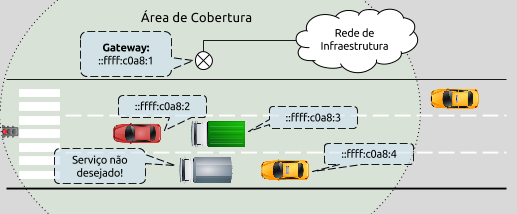
\includegraphics[scale=.8]{figuras/cap3/38AtribuicaoIPv6RSU}
		\caption{\label{fig_38}Atribuição de IPv6 por uma unidade de acostamento}
	\end{figure}
	
	\par Cada dispositivo WAVE que oferecer serviços IP deverá suportar endereços locais, globais e de \textit{multicast} para IPv6, seguindo a norma IETF RFC 2373. 
	
	\par A configuração IP do padrão WAVE será realizada por meio de WSAs utilizando um canal de serviço, já que o canal de controle não podem ter tráfego IP. 
		
	\par Os dispositivos WAVE podem implementar qualquer outro protocolo da IETF (Internet \textit{Engineering Task Force}), mas devem ser tomadas precauções para que a interoperabilidade não seja afetada com outros dispositivos da Rede Veicular.
	
	\par Portanto, conforme visto nesta seção, a comunicação entre veículos nas camadas de rede e transporte pode ser feita via protocolos IPv6 ou WSMP. O protocolo WSMP é utilizado para troca de informações \textit{ad hoc} dentro da rede veicular, já o IPv6 é empregado em situações quando a troca de dados necessita de uma rede de infraestura.
	
	\section{Camada de Aplicação}
	
	\par Utilizando a troca de mensagens na camada de aplicação WAVE, softwares podem ser desenvolvidos para gerar funcionalidades voltadas à segurança, informação e entretenimento nas redes veiculares.
	
	\subsection{Aplicações de Segurança e Informação}
	
	\par A SAE, por meio da norma SAE J2735, propôs três diferentes conjuntos de mensagens para aplicações de redes veiculares. Estas mensagens foram propostas de modo pragmático, utilizando notação ASN.1 e regras de codificação nos formatos DER (\textit{Distinguished Encoding Rules}) e XML. É importante salientar que o padrão SAE J2735 não implementa uma aplicação ou sistema e sim ilustra como as mensagens da camada de aplicação são codificadas e decodificadas.
	
	\par Como até então não haviam APIs (\textit{Application Program Interface}) desenvolvidas para as camadas do modelo WAVE e nem protótipos de placas de rede, o padrão realizou testes de construção e decodificação de mensagens broadcast WSM utilizando \textit{sockets} Berkeley como API padrão, além do protocolo de transporte UDP representando o WSMP em uma placa de rede \textit{Ethernet}. Entidades de gerenciamento WAVE foram criadas no código.
	
	\par Os conjuntos de mensagens implementados no padrão SAE J2735 são:

	\begin{itemize}
		\item BSM (\textit{Basic Safety Message} ou Mensagem Básica de Segurança)
		\item RSA (\textit{RoadSide Alert} ou Mensagens de Alerta de Acostamento)
		\item Mensagens Sensoriais de Veículos (\textit{Probe Vehicle Message} ou PVM)
	\end{itemize}
	
	\par As BSMs são mensagens para aplicações de segurança em veículos. Estas aplicações utilizariam o fluxo de dados de BSMs provenientes de veículos nas redondezas para detectar potenciais eventos de risco. As BSMs fornecem aos veículos conhecimento da posição, velocidade e direção dos veículos nas imediações. Estas mensagens de segurança possuem grupos de PSIDs para dados específicos. Conforme mostrado \autoref{tab_9}, para BSMs contendo dados de alta precisão o grupo PSID utilizado é o 0x20. Para veículos com dados não tão acurados, o grupo de PSID utilizado é o 0x21. 
	
	\par Como exemplo, foi proposta uma aplicação de um sistema de frenagem inteligente que detecta potenciais colisões traseiras mediante algoritmos de detecção. Após detectado o potencial risco de colisão, o condutor é alertado passivamente ou o sistema realiza ações corretivas, como desabilitar o “piloto automático”, fortalecer os freios e pré-tensionar os cintos de segurança. 
	
	\par Outros exemplos de aplicações podem aproveitar-se das mensagens básicas de segurança para os mais diversos fins, como:
	\begin{itemize}
		\item Aplicações para aviso de pontos cegos;
		\item Aplicações para cooperação entre pilotos automáticos;
		\item Aplicações para prevenção de colisões;
		\item Aplicações para advertir presença de veículos de emergência;
		\item Aplicações para alertar mudança de faixa;
		\item Aplicações para detecção pré-colisão
	\end{itemize}
	
	\par As RSAs são mensagens de broadcast voltadas à aplicações de informação. Estas informações são voltadas principalmente às condições de tráfego e são propagadas principalmente por veículos de segurança pública ou por unidades de acostamento (RSUs ou \textit{RoadSide Units}) que entregam dados de Centros de Gerenciamento de Tráfego. Os tipos de dados transmitidos por RSAs são geralmente de atrasos em percursos causado por engarrafamentos, recálculo de rotas, informações de sinalização, incidentes, pontos de interesse, etc.
	
	\par As PVMs são mensagens usadas por múltiplas aplicações. Os veículos coletam dados próprios, de condições de pistas e de tráfego por meio de seus sensores em determinados intervalos de tempo. Esta gama de dados coletada é chamada de \textit{snapshot}. Estes dados são combinados em mensagens e transmitidos para unidades de acostamento (RSUs) que aceitam estes \textit{snapshots}  quando dentro de seu alcance. Das RSUs, os dados são enviados para Centros de Gerenciamento de Tráfego e Provedores de Serviços a fim de outros usuários móveis serem abastecidos destas informações.
	
	\par Como exemplo, os sensores de dados retornam informações como:
	
	\begin{itemize}
		\item Aceleração Vertical e Horizontal
		\item Altitude
		\item Ângulo do volante
		\item Calibragem dos pneus
		\item Clima (Sol, Chuva, Radiação)
		\item Coeficiente de Fricção com a pista
		\item Direção de obstáculo
		\item Direção do veículo
		\item Distância de obstáculo
		\item Latitude
		\item Longitude
		\item Pressão atmosférica
		\item Status do Sistema de Freio
		\item Taxa de derrapagem
		\item Temperatura
		\item Tempo e hora
		\item Tipo de veículo
		\item Velocidade
	\end{itemize}

	\subsection{Protocolo para Coleta eletrônica de Taxas}

	\par Baseando-se no padrões IEEE 1609.3, IEEE 1609.4, IEEE 1609.11, ISO 14906 e ISO 15628, um sistema de pagamento eletrônico para redes veiculares foi proposto como aplicação em redes veiculares. As normas citadas estabelecem as diretrizes para alcance de confiabilidade e segurança no pagamento. 
	
	\par Para transações eletrônicas ocorrerem com sucesso, deve-se garantir uma associação inequívoca de cada pagador com seu veículo para que não haja erros no processamento do pagamento durante a curta presença dos veículos ao atravessarem os postos de pagamento eletrônicos (que podem ser de estacionamentos ou pedágios utilizando-se ou não de cancelas eletrônicas). Isto é, se cinco veículos passarem por um posto eletrônico de pedágio e apenas 4 pagamentos forem registrados, o sistema deve determinar qual veículo evadiu o pagamento. Fotografias dos veículos em conjunto com o registro de transações realizadas podem evidenciar possíveis evasões.
	
	\par A \autoref{fig_39} apresenta uma aplicação de um sistema de pagamento eletrônico para pedágios. Com duas unidades de acostamento (RSUs) de três antenas na praça de pedágio, a primeira antena de cada unidade é sintonizada no Canal de Controle (CCH) para enviar \textit{frames} “despertadores” para as unidades móveis próximas.
	
	%INSERIR Figura 39 Aplicação de pedágio
	\begin{figure} [H]
		\centering
		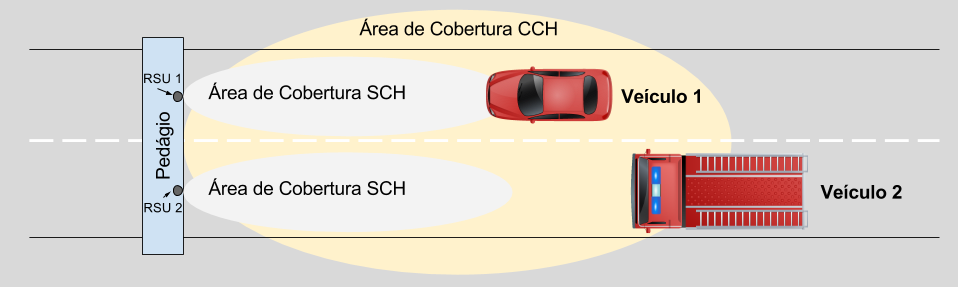
\includegraphics[scale=.4]{figuras/cap3/39AplicacaoPedagio}
		\caption{\label{fig_39}Aplicação de pedágio}
	\end{figure}
	
	\par A antena no CCH também envia Mensagens de Anúncio que divulgam a presença da praça de pedágio no percurso e entregam os parâmetros do serviço como o canal, método de acesso ao canal, PSID e demais parâmetros.
	
	\par Quando uma unidade móvel (OBU) recebe o anúncio de um Serviço de Coleta Eletrônica de Taxas, a entidade de gerenciamento WAVE (WME) troca para o canal de serviço (SCH) e método de acesso descritos pelo anúncio, que no exemplo é respectivamente SCH 182 com acesso contínuo. Informações da aplicação na \autoref{tab_4}.
	
	\par As duas antenas restantes se responsabilizam pelo SCH a fim de executar a troca de mensagens com OBUs na área de cobertura. Logo, as camadas de aplicação da RSU e das OBUs dentro da área de cobertura trocam informações de pagamento.
	
	% TABELA Aplicação de Pedágio
	
	\begin{table}[H]
		\centering
		\renewcommand{\arraystretch}{1.5}
		\begin{tabular}{|c|c|p{6cm}|} \hline
			\textbf{Parâmetro} &	\textbf{Valor} &	\multicolumn{1}{c|}{\textbf{Descrição}} \\ \hline
			Endereço MAC Destinatário & broadcast & WSA é um broadcast \\ \hline
			Tipo WSA & não segura & WSA não assinada \\ \hline
			PSID & 0x01 & Coleta eletrônica de taxas \\ \hline
			Número do Canal & 182 &	Identifica o número do canal a ser utilizado pelo serviço \\ \hline
			Tipo de Acesso ao Canal & contínuo & Usuário deve trocar para SCH imediatamente \\ \hline
			Taxa de repetição & 250 &	WSA transmitida 5 vezes a cada 100ms \\ \hline
			Serviço de IP & falso & Utiliza-se WSMP \\ \hline
		\end{tabular}	
			\caption{\label{tab_4}Dados da aplicação de pedágio}
	\end{table}			
	
	\par É importante acrescentar que a realização do pagamento eletrônico leva em consideração que os veículos tenham algum mecanismo de pagamento cadastrado e funcional.

	\par O próximo capítulo irá discorrer sobre as diversas formas de avaliar novas tecnologias.

%-------------------------------------------------------------
	\newpage
	\chapter{Abordagem Avaliativas}
	\label{chap:Abor_Aval}
	
	\par Toda e qualquer tecnologia precisa ser testada utilizando abordagens avaliativas antes de entrar em caráter de produção no mercado. Abordagens avaliativas são métodos distintos de pensar, desenhar e conduzir atividades de avaliação. A utilização de abordagens avaliativas na ciência cresceu consideravelmente a partir de um movimento internacional encorajando práticas científicas baseadas em evidências. A abordagem avaliativa empregada em determinada tecnologia é fundamental para antecipar possíveis inconvenientes ou conflitos antes desta entrar em fase de produção.
	
	\par Para a implementação de tecnologias em redes veiculares, há um conjunto de abordagens avaliativas que podem ser empregadas que vão desde coletas da análise conjuntos de dados, passando por simulações até experimentos no mundo real. 
	
	\par A utilização de ferramentas de simulação foi a abordagem experimental escolhida por este trabalho para o experimento de redes veiculares em estudo de caso. Banks et al (2005) cita diversos propósitos em que simulações são ferramentas apropriadas de avaliação, entre as quais se destacam para o escopo deste projeto:
	
	\begin{itemize}
		\item O conhecimento alcançado durante o desenho do módulo de simulação é de valor considerável para a sugestão de aprimoramentos no sistema sob investigação;
		\item A simulação pode ser usada como instrumento pedagógico para reforçar solução analíticas;
		\item A simulação pode ser utilizada para experimentar novos conceitos antes da implementação, como também preparar para situações inesperadas;
		\item A simulação pode testar diferentes recursos para a máquina que podem auxiliar em uma futura determinação de requisitos.
	\end{itemize}
	
	\par Banks et al (2005) acrescem que as simulações devem portar dados de saída que correspondam diretamente àqueles gravados em mundo real para que suposições duvidosas não sejam criadas a seu respeito. O processo avaliativo envolvido na simulação é de caráter observativo. Um conjunto de dados de entrada e características é dado, o módulo é executado para então resultar em cenários a serem avaliados.
	
	\par Pegden et al (1995) citam vantagens no desenvolvimentos de módulos para simulação:
	
	\begin{itemize}
		\item Novas políticas, regras, fluxos, procedimentos organizacionais e operacionais podem ser explorados sem interromper as operações em andamento no mundo real;
		\item Novos esboços de hardware podem ser testados sem necessidade de reservar recursos para sua aquisição;
		\item Hipóteses sobre como certos fenômenos ocorrem podem ser testados;
		\item O tempo pode ser compresso ou expandido para permitir aceleração ou desaceleração dos fenômenos sob investigação;
		\item A compreensão das interações, das variáveis e sua importância pode ser aprimorada na observação de simulações;
		\item A simulação permite analisar gargalos a fim de descobrir onde há processos atrasando o desempenho do sistema;
	\end{itemize}
	
	\par Confome corroborado também por Olariu \& Weigle (2009), a maneira mais apropriada de se avaliar o desempenho de uma rede é desenvolvendo simulações que forneçam resultados mais próximos de observações do mundo real.
	
	\par Para se avaliar o funcionamento de simulações em redes veiculares, há de se integrar um conjunto de softwares que incorporem o aspecto de arquitetura de redes de comunicações juntamente com softwares que produzam a mobilidade e a aleatoriedade existente em ambientes veiculares. Isto é, para a simulação de redes veiculares é necessário integrar:
	
	\begin{itemize}
		\item Um software de Simulação de Redes
		\item Um software de Simulação de Tráfego Urbano
		\item Um \textit{Middleware} que coordene comunicação bidirecional 
	\end{itemize}
	
	\par Cheng et al (2015) analisaram um considerável número de softwares destes grupos e coletaram características individuais para concluir quais seriam os conjuntos de softwares de simulação de redes veiculares que trariam resultados mais próximos à realidade. No fim de cada seção seguinte, serão listados requisitos importantes para a escolha de um software de cada tipo e anunciado o software escolhido para o estudo de caso deste trabalho.
	
	\section{Softwares de Simulação de Redes}
	
	\par Os softwares de simulação de redes auxiliam no desenvolvimento de novos projetos de redes. Alguns destes softwares oferecem interface gráfica  (\textit{Graphical User Interface} ou  GUI), além de módulos de tráfego para diversos protocolos, módulos de perda de pacotes, de atenuação de sinal, de tipos de cabos e protocolos de rede desejados. Fabricantes de dispositivos de rede como a Cisco utilizam de softwares de simulação para demonstrar o funcionamento de seus produtos.
	
	\par Através das simulações desempenhadas em softwares de simulação de redes, o desempenho de diferentes configurações de redes pode ser comparado, sendo possível reconhecer e resolver problemas de desempenho sem a necessidade de conduzir testes de campo que seriam potencialmente caros. A simulação de redes é amplamente utilizada por pesquisadores na avaliação do comportamento de protocolos recém desenvolvidos e por projetistas de rede para desenhar e avaliar novos projetos de rede.

	\par Na maioria dos casos, softwares de simulação de redes são baseados no conceito de modelagem de eventos discretos, que consiste na mudança de estado de sistemas apenas no instante que um determinado evento ocorrer. Para os demais instantes de tempo, nada muda no sistema. Os modelos de simulação utilizam métodos numéricos, isto é, procedimentos computacionais para lidar com modelos matemáticos.
	
	\par Como redes veiculares utilizam de comunicações sem fio, nem todos os softwares de simulação de redes podem ser utilizados para a construção deste cenário de simulação exceto aqueles que apresentarem módulos de simulação de redes veiculares integrados ou externos.
	
	\par Cheng et al (2015) analisaram softwares de simulação de redes, distinguindo-os conforme mostrado na \autoref{tab_5}. 
	
	%INSERIR Tabela comparativa de softwares de simulação de redes
	\begin{table}[H]
		\renewcommand{\arraystretch}{1.5}
		\centering
		\begin{tabular}{|p{1.97cm}|p{1.72cm}|p{1.73cm}|p{1.66cm}|p{1.66cm}|p{1.77cm}|p{1.78cm}|p{1.77cm}|}
			\hline
			{\textbf{Simulador de Redes}} & \textbf{OPNET} & {\textbf{ns-2}} & {\textbf{ns-3}} & \textbf{J-Sim} & \textbf{OMNET} & \textbf{SWANS} \\ \hline
			Licença & Comercial & GNU GPLv2 & GNU GPLv2 & BSD License & Acadêmica, Comercial & Acadêmica \\ \hline
			Linguagem de Programação escrita & - & C++ & C++ & Java & C++ & Java \\ \hline
			Linguagem da simulação & C, C++ & C++, OTcl & C++, Python & Java, Tcl, Perl, Python & C++, NED & Java, Python \\ \hline
			Possui GUI & Sim & Não & Não & Não & Sim & Não \\ \hline
			Sistemas Suportados & Windows & Linux, OS X, Solaris, Windows & Linux, Windows & Windows, OS X, Linux & Windows, OS X, Linux & Windows, OS X, Linux \\ \hline
			Código Fonte & Apenas para nós de simulação & Sim & Sim & Sim & Sim & Sim \\ \hline
			Tecnologias sem-fio & \textit{WiFi}, LTE, UMTS, \textit{WiMAX}, Zigbee, \textit{Satellite} & \textit{WiFi}, \textit{Satellite}, \textit{Cellular} & \textit{WiFi}, \textit{WiMAX}, LTE & \textit{WiFi} & Nenhuma (Apenas módulos externos) & \textit{WiFi} (IEEE 802.11b)  \\ \hline
			Módulo de mobilidade & Não & Não & Não & Não & Não & Não \\ 
			\hline
		\end{tabular}
			\caption{Comparação entre softwares de simulação de redes}
			\label{tab_5}				
	\end{table}

	\par Para determinar o software de simulação de redes para o desenvolvimento de estudo de caso, o processo de escolha atendeu os seguintes requisitos:
	
	\begin{enumerate}
		\item O software possui uma interface gráfica amigável para compreensão ágil de seu escopo de desenvolvimento;
		\item O software apresenta portabilidade para diversos sistemas operacionais;
		\item O software possui licença acadêmica ou aberta;
		\item O software permite a simulação modelos de redes veiculares;
		\item O software possui boa reputação na campo acadêmico com uma comunidade ativa.
	\end{enumerate}
	
	\par O software de simulação que atendeu melhor tais critérios foi o \textbf{OMNET++}. Este software é descrito com maiores detalhes na próxima seção.
	
	\subsection{OMNET++}
	
	\par O OMNET++ é um software de simulação de eventos discretos que possui licença acadêmica pública. As bibliotecas componentes deste software foram construídas na linguagem C++. 
	Este software apresenta características de modularidade, extensibilidade e portabilidade. A primeira e segunda características dizem respeito à possibilidade de integração com outras  bibliotecas, tornando possível simular, por exemplo, redes de sensores, redes \textit{ad hoc}, protocolos de Internet, redes fotônicas. Isto fez do OMNET++ conhecido na comunidade científica como um software de simulação de redes, justamente por conter bibliotecas de simulação de redes como MiXiM, INET e VEINS. A portabilidade do \textit{framework} é vista no suporte à diversas plataformas, como os sistemas Windows, Linux e Mac OS X.
	
	\par A interface gráfica do software é baseada no Eclipse, o que torna a ambientação mais rápida para desenvolvedores acostumados a trabalhar com esta IDE. A \autoref{fig_40} apresenta a IDE do OMNET++.

	%INSERIR Figura 40 Interface OMNET++
	\begin{figure} [H]
		\centering
		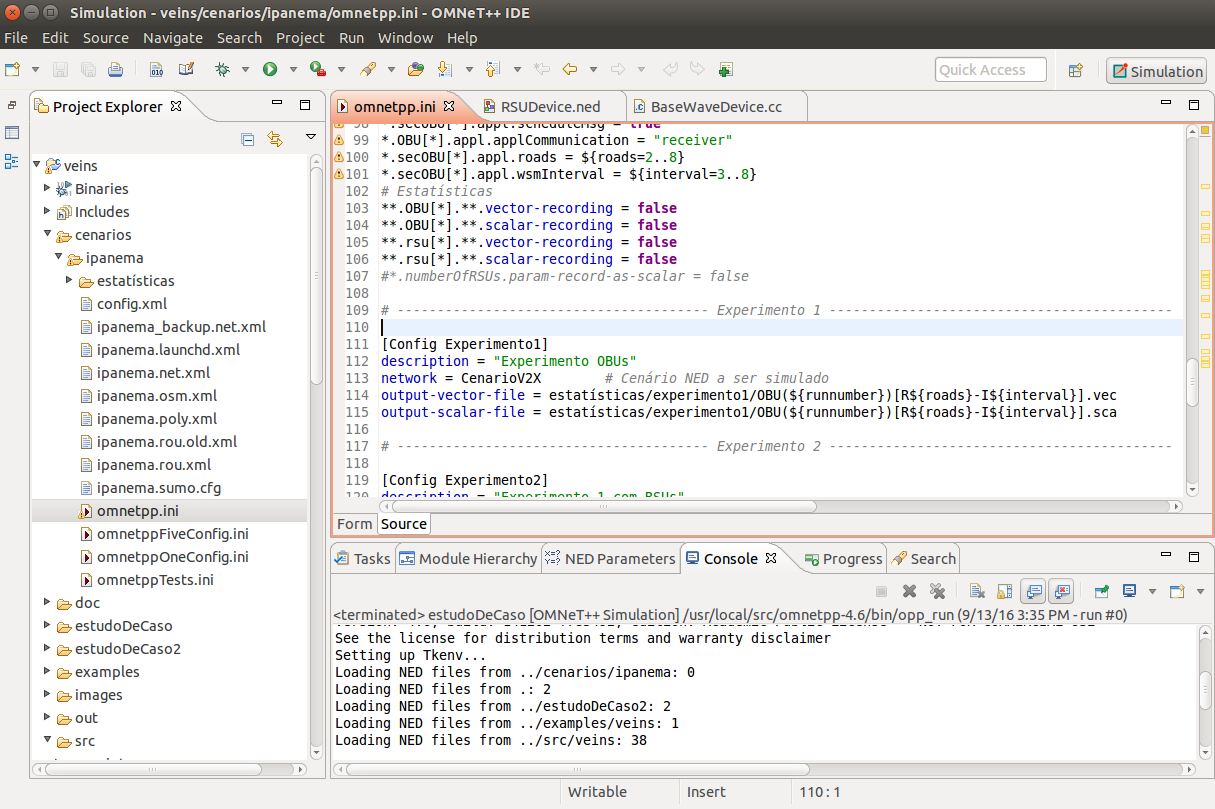
\includegraphics[scale=.37]{figuras/cap4/40InterfaceOMNET}
		\caption{\label{fig_40}Interface OMNET++}
	\end{figure}
	
	\par O software possui três ambientes de execução, sendo duas gráficas. O Cmdenv, que executa as simulações em lote pela linha de comando. O TkEnv, que é o mais tradicional e permite a virtualização de objetos em duas dimensões (\autoref{fig_41}). E por fim, o recém incorporado QtEnv permite a simulação gráfica de objetos em três dimensões, utilizando a biblioteca do \textit{openscenegraph} (\autoref{fig_42}).
	
	% INSERIR FIGURA 41 INTERFACE GRÁFICA do TKEnv
	\begin{figure} [H]
		\centering
		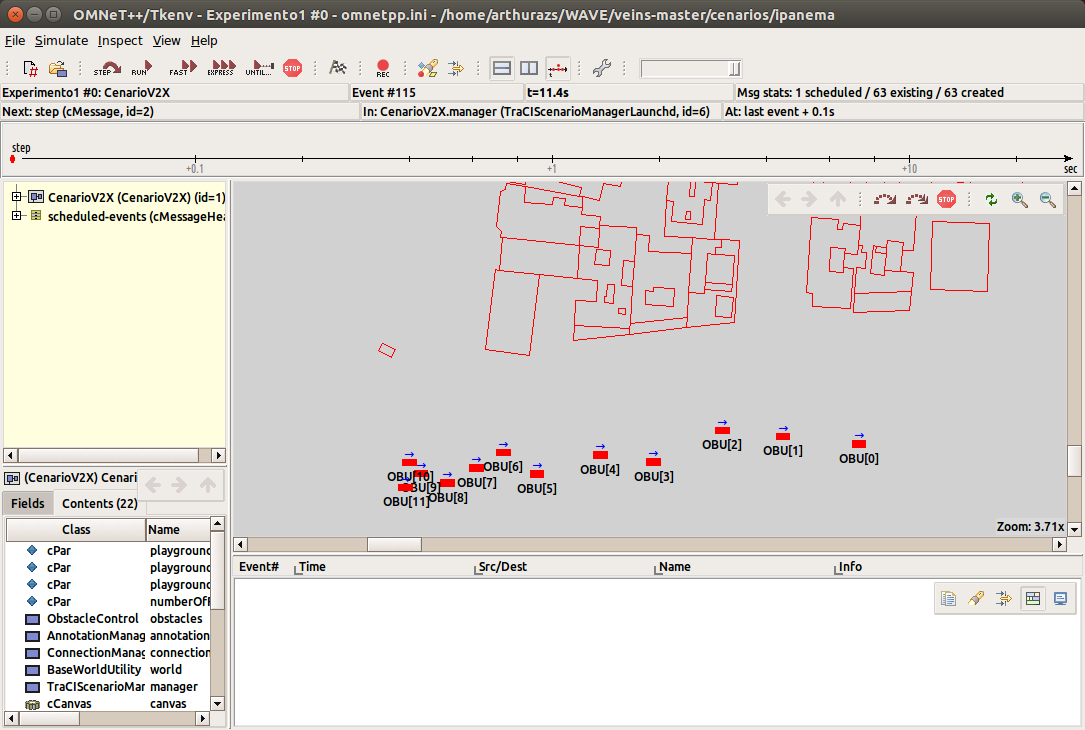
\includegraphics[scale=.4]{figuras/cap4/41InterfaceTKENV}
		\caption{\label{fig_41}Interface TkEnv}
	\end{figure}
	
	% INSERIR FIGURA 42 INTERFACE GRÁFICA do QTEnv
	\begin{figure} [H]
		\centering
		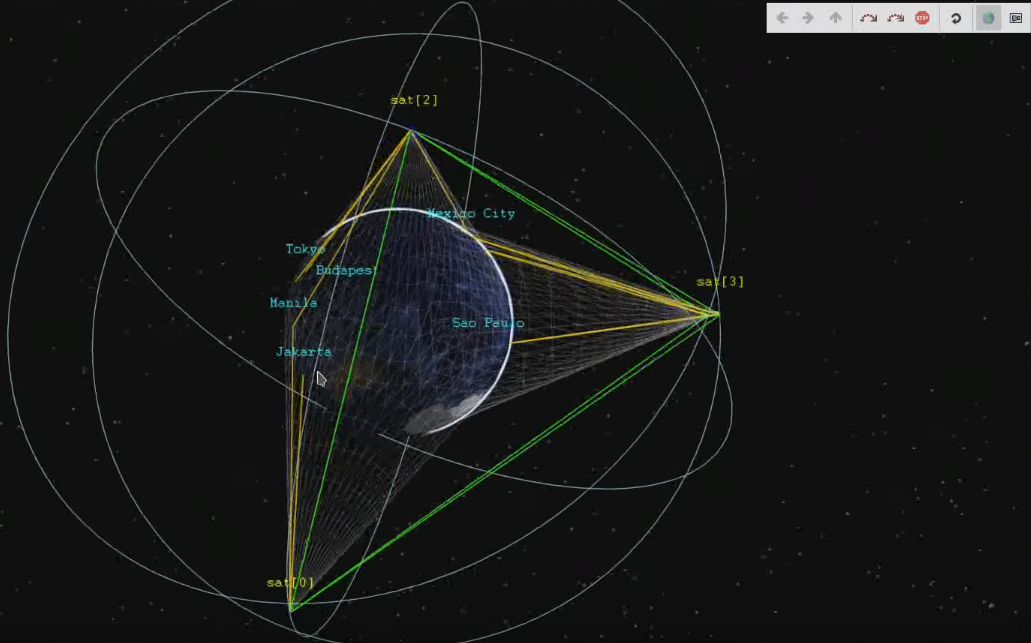
\includegraphics[scale=.4]{figuras/cap4/42InterfaceQTENV}
		\caption{\label{fig_42}Interface QtEnv}
	\end{figure}
		
	\newpage
		
	\par Além de realizarem a simulação gráfica, o TkEnv e QtEnv fazem o registro de eventos. Há GUIs específicas para os registros dos módulos (\autoref{fig_43}) e de pacotes enviados entre os nós (\autoref{fig_44}).
	
	%INSERIR Figura 43 ModuleLog
	\begin{figure} [H]
		\centering
		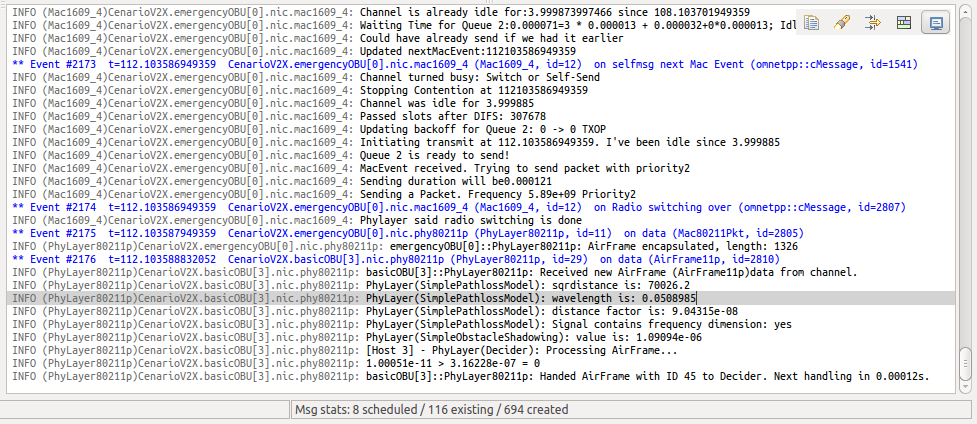
\includegraphics[scale=.4]{figuras/cap4/43ModuleLog}
		\caption{\label{fig_43}Module Logger}
	\end{figure}
	
	%INSERIR Figura 44 MessageLog
	\begin{figure} [H]
		\centering
		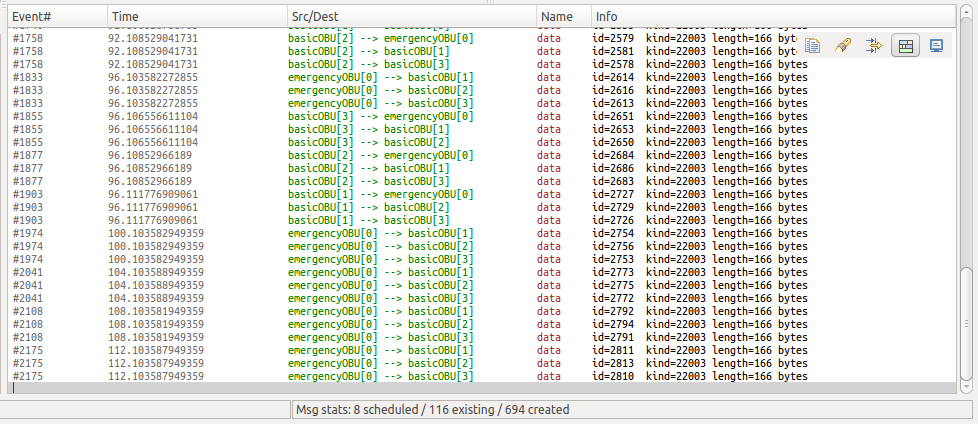
\includegraphics[scale=.4]{figuras/cap4/44MessageLog}
		\caption{\label{fig_44}Message Logger}
	\end{figure}
		
	\par O OMNET++ fornece uma arquitetura de componentes para os módulos a serem simulados. Este componentes são programados em C++, e integrados em uma linguagem de alto nível chamada NED. O principal objetivo da linguagem NED é descrever as topologias de rede a serem utilizadas. Os módulos descritos podem ser estendidos ou reutilizados por qualquer outro externo. A GUI do OMNET++ também pode ser estendida.
	
	\section{Software de Simulação de Tráfego}
	
	\par Os softwares de Simulação de Tráfego são utilizados na Engenharia de Transportes e ajudam a descrever o desenho do trânsito de uma cidade da forma mais eficiente possível. Estes \textit{softwares} utilizam modelos de tráfego que se classificam em três tipos no que diz respeito à granularidade do fluxo:
	
	\par \textbf{Modelos Macroscópicos} medem o tráfego em larga escala, tratando o tráfego como um líquido. O nível de detalhamento do fluxo de tráfego nestes modelos é baixo, não existindo interesse por cada veículo e sim pelo fluxo.
	
	\par \textbf{Modelos Mesoscópicos} medem o tráfego em uma escala menor, se preocupando com o movimento de pelotões de veículos. Utilizam funções velocidade-densidade para modelar o comportamento destes modelos. 
	
	\par \textbf{Modelos Microscópicos} medem o tráfego de veículos em uma escala individual em que cada veículos é um traço, portanto o nível de detalhamento do fluxo de tráfego nestes modelos é alto.
		
	% INSERIR Tabela de tipos de modelos de tráfego por granularidade
	\begin{table}[H]
		\centering
		\renewcommand{\arraystretch}{1.5}
		\label{tab_6}
		\begin{tabular}{|c|c|}
			\hline
			\textbf{Granularidade do Modelo de Tráfego} & \textbf{Frameworks} \\ \hline
			Macroscópica & METACOR \\ \hline
			Mesoscópica & CONTRAM \\ \hline
			Microscópica & SUMO \\ \hline
		\end{tabular}
		\caption{Modelos de tráfego por granularidade}
	\end{table}
	
	\par Para a simulação de redes veiculares, foi notado que o modelo de tráfego deveria se preocupar com a modelagem individual de transmissão de rádio entre os nós, necessitando das posições, dos vetores e de ações exatas de nós individuais. Modelos com pelotões de veículos e ou tendências macroscópicas de tráfego não se adequariam às  comunicações inter veiculares. 
	
	\par Seguindo o critério estabelecido acima foi visto que há diversos modelos de microtráfego urbano implementados. Segundo conclusão de Brockfeld \& Wagner (2004), todos os modelos microscópicos de simulação apresentam um mesmo valor de acurácia como modelos de mobilidade. Isto inclui os modelos \textit{Cellular Automaton}, \textit{Car-following} e IDM/MOBIL.
	
	\par O processo de escolha de software de simulação de trânsito para o desenvolvimento de estudo de caso atendeu os seguintes critérios:
	
	\begin{enumerate}
		\item O software apresenta um modelo de trânsito com granularidade microscópica;
		\item O software apresenta portabilidade para diversos sistemas operacionais;
		\item O software é de licença acadêmica ou aberta;
		\item O software permite a simulação modelos de redes veiculares;
		\item O software possui boa reputação na campo acadêmico com uma comunidade ativa.		
	\end{enumerate}

	\par O software de simulação que cumpriu estes critérios foi o \textbf{SUMO} (\textit{Simulator of Urban Mobility}). Este software é descrito em maior detalhe na próxima seção.
	
	\subsection{\textit{Simulator of Urban Mobility}}
	
	\par O SUMO é um software de simulação de tráfego urbano desenvolvido pelo Instituto de Sistemas de Transportes da Alemanha. É um sistema de código aberto, portátil e foi projetado para lidar com grandes redes rodoviárias.
	
	\par O SUMO faz a modelagem de tráfego microscópica. Cada veículo tem sua própria rota e se move individualmente na rede. As simulações são determinísticas por padrão, contudo há um conjunto de configurações que introduzem aleatoriedade no software.
	
	\par As bibliotecas do SUMO são majoritariamente em C++. Algumas ferramentas de apoio foram codificadas em Python e XML.
	
	\par No SUMO há a possibilidade de criar os próprios mapas a partir de códigos XML, importar mapas de outros softwares de simulação ou mesmo de sites como o \textit{Openstreetmaps}. Isto é, cidades inteiras podem ter seus tráfegos simulados no SUMO.

	% INSERIR FIGURA DE IDE DO SUMO
	\begin{figure} [H]
		\centering
		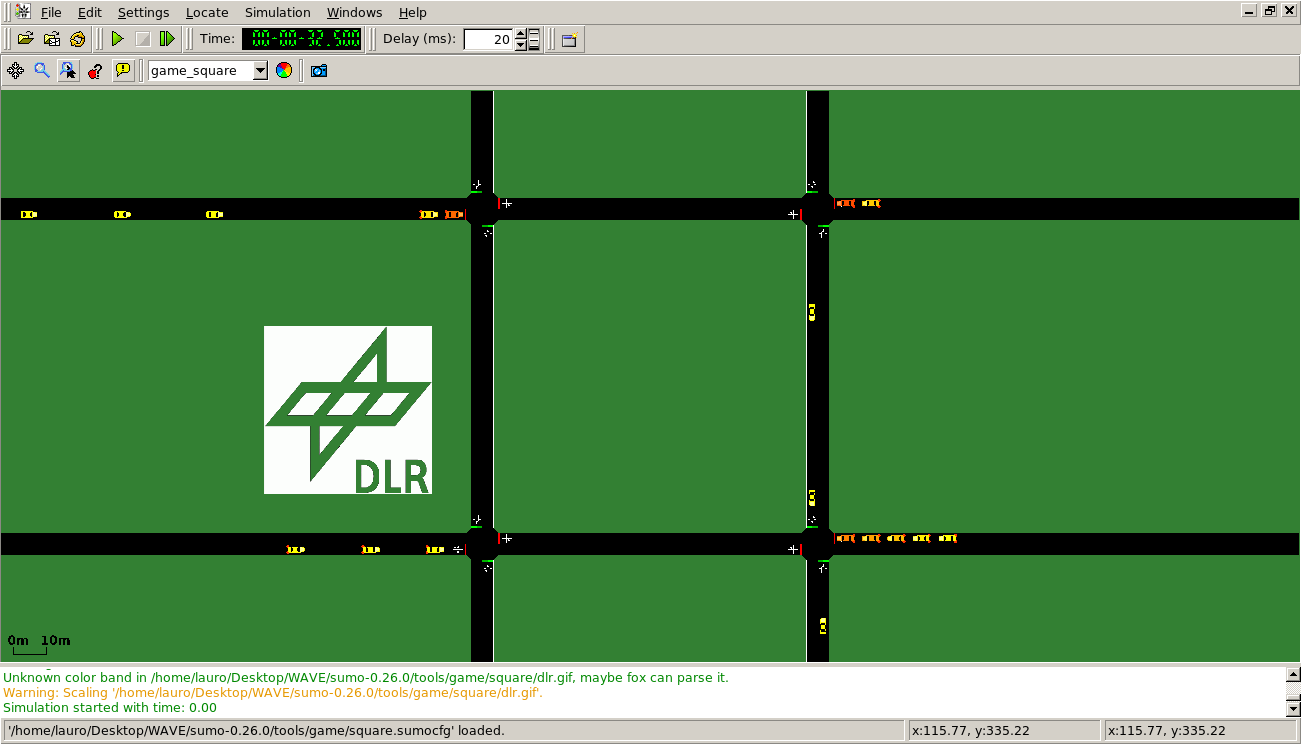
\includegraphics[scale=.3]{figuras/cap4/45InterfaceSUMO}
		\caption{\label{fig_45}Interface SUMO}
	\end{figure}
	
	\par Além das características já citadas acima, o SUMO também permite:
	
	\begin{itemize}
		\item A criação de ruas de múltiplas faixas, com regras de trânsito específicas por faixa e com mudança de faixa permitida aos veículos;
		\item Regras e temporização de semáforos, sendo possível criar algoritmos que os controlem;
		\item Criação de fluxos e rotas para veículos seguirem;
		\item Escolha de diferentes tipos de veículos (carros \textit{sedan}, \textit{hatch}, ambulâncias, motos, ônibus, caminhões, etc)
		\item Configuração de regras de trânsito específicas (mão inglesa, vias com preferência, etc.)		
	\end{itemize}
	
	\par Uma das características fundamentais do SUMO é que este pode interoperar com outras aplicações em tempo de execução transferindo dados da simulação para o processamento em outros sistemas. Isto também possibilita que o SUMO receba dados provenientes de outros sistemas, alterando diretamente no resultado de simulações e introduzindo mais um fator de aleatoriedade.
	
	\section{Middleware de Integração}
	\label{sec:MiddleIntegra}
	
	\par Para integrar aplicações de simulações de rede e de tráfego com troca de informações bidirecional, é necessário ter um \textit{framework} que faça a interface entre estes software e ofereça bibliotecas de suporte. O \textit{framework} escolhido para esta função foi o VEINS, que será abordado com maiores detalhes na próxima seção.
	
	\subsection{\textit{Vehicles in Network Simulation}}
	
	\par VEINS (\textit{Vehicles in Network Simulation} ou Veículos em Simulação de Redes) é um \textit{framework} para o OMNET++ que contém bibliotecas para simulação de redes veiculares e faz a comunicação entre o OMNET++ e o SUMO. Sua arquitetura é mostrada na \autoref{fig_451}. O \text{framework} em questão tem o módulo de mobilidade (Mobility) ligado ao SUMO (Road Traffic Simulation) através de uma interface de controle de tráfego (TraCI) que utiliza uma porta TCP para comunicação. Isto faz com que cada simulação de rede veicular no VEINS execute os dois simuladores em paralelo: OMNET++ e SUMO.

	% INSERIR FIGURA DE IDE DO SUMO
	\begin{figure} [H]
		\centering
		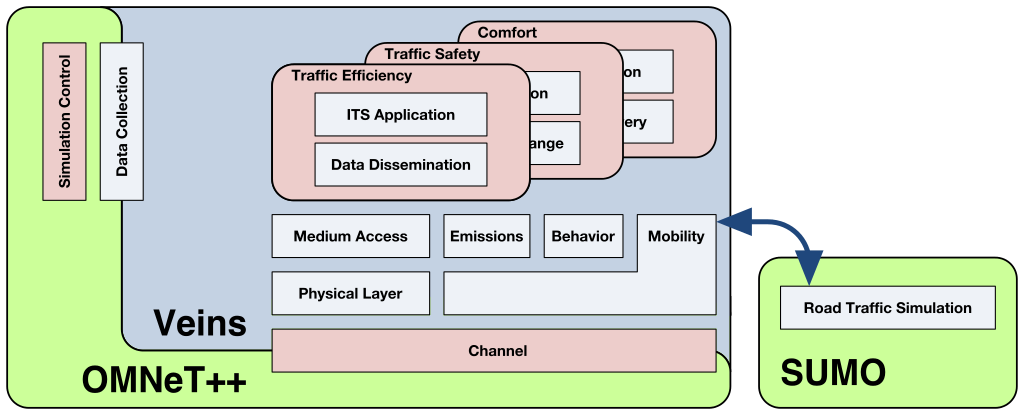
\includegraphics[scale=.8]{figuras/cap4/451Veins}
		\caption{\label{fig_451}Arquitetura do \textit{framework} VEINS}
	\end{figure}
	
	\par Este \textit{framework} foi escolhido por oferecer as seguintes características:
	
	\begin{itemize}
		\item Possui código 100\% aberto, promovendo extensibilidade irrestrita;
		\item Permite a reconfiguração de rotas dos veículos do SUMO em tempo de execução em reação ao envio de pacotes de rede;
		\item Baseado nos padrões IEEE 802.11p e IEEE 1609.4 para descrever as camadas física e de rede, incluindo operação multi-canal, QoS, efeitos de ruído e interferência;
		\item Inclui módulos de redes de celular, como LTE;
		\item Permite a importação de cenários do \textit{OpenStreetMap}, incluindo prédios, limites de velocidade, semáforos, etc;
		\item Permite empregar módulos de atenuação de sinal causados por veículos e prédios;
		\item Gera dados com uma diversidade de métricas, incluindo tempo total de trajeto, emissões de dióxido de carbono, velocidades máxima e mínima. A geração de novos conjuntos de dados é possível extendendo o código do \textit{framework};
		\item Possui uma base ampla de usuários.
	\end{itemize}
	
	\par O VEINS utiliza uma relevante coleção de módulos aplicados em suas simulações de redes veiculares. Estes módulos servem como base para a construção de uma simulação específica, utilizando apenas aqueles relevantes para o cenário concebido. Alguns desses módulos são:
	
	\begin{description}
		\item[O MiXiM] é utilizado para modelagem precisa da camada física, trabalhando com distribuição da potência de transmissão por tempo e distância;
		\item[O TraCI] (\textit{Traffic Control Interface} ou Interface de Controle de Tráfego) é uma interface que transforma os veículos do SUMO em nós de rede do OMNET++. Este modulo é utilizado pra monitorar o fluxo da simulação no SUMO, atualizando informações sobre a mobilidade do nó (posição, velocidade, direção) no OMNET++, baseado nos comportamentos dos veículos. Este módulo permite a reconfiguração de rotas dos veículos em tempo de execução e que VEINS e SUMO trabalhem em conjunto trocando mensagens de status por intermédio de uma porta TCP aberta;
		\item[Os módulos IEEE 802.11p e IEEE 1609.4 DSRC/WAVE] realizam uma modelagem mais precisa das camadas física e de rede WAVE, incluindo técnicas de modulação e coordenação de canal, QoS conforme EDCA. Este módulo também inclui a manipulação de WSM, quadros de gerenciamento (\textit{beacons}), WSAs, BSMs, etc.
		\item[O módulo \textit{Two-Ray Interference}] gerencia a perda de pacotes em diferentes distâncias e trabalha com a propagação de mensagens entre os carros, a distância máxima de uma mensagem enviada por um único nó e a distância máxima da mesma mensagem propagada por intermédio de outros nós;
		\item[O módulo \textit{Obstacle Shadowing}] monitora os obstáculos que podem interferir a propagação da mensagem.
	\end{description}
	
	\par A vasta biblioteca do VEINS em C++ contém classes que exercem diversos papéis no contexto de simulações veiculares. O código fonte destas classes pode ser alterado ou estendido para a obtenção de resultados mais específicos. Quando importados no OMNET++, tais classes são encontradas no diretório src/veins/modules do projeto VEINS. Algumas classes relevantes deste \textit{framework} são explicadas em detalhe na \autoref{tab_7}. 
	
	% INSERIR Tabela Módulos do VEINS
	\begin{table}[H]
		\renewcommand{\arraystretch}{1.5}
		\centering
		\begin{tabular}{|l|p{10.5cm}|}
			\hline
			\multicolumn{1}{|c|}{\textbf{Classes}} & \multicolumn{1}{c|}{\textbf{Detalhes}} \\ \hline
			TraCICommandInterface & Classe que controla o comportamento dos veículos no SUMO. É possível enviar comandos de mudança de faixa, velocidade, rota, etc. Esta classe simula os comportamentos de um motorista. \\ \hline
			TraCIScenarioManager & Classe que cria e gerencia o nó de rede de cada veículo. \\ \hline
			TraCIMobility & Classe que controla a situação dos diversos sensores do veículo. É possível obter informações como quilometragem, velocidade, emissão de carbono, estado atual (em deslocamento, estacionando, parado, etc), entre outros. Esta classe simula o funcionamento dos diversos sensores de um carro. \\ \hline
			Consts80211p & Arquivo cabeçalho que reúne constantes relacionadas aos padrões IEEE WAVE, como o tempo para alterar do modo transmissão (Tx) para recepção (Rx), intervalo de guarda, número dos canais, etc. \\ \hline
			ConstsPhy & Arquivo cabeçalho que reúne constantes da camada física de um rádio. Contém informações sobre modulação de sinal, largura de banda, etc. \\ \hline
			PhyLayer80211p & Classe que implementa módulos de modelos analógicos e faz  pequenas alterações no módulo base MiXiM. \\ \hline
			Mac1609\_4 & Classe que reúne as funções da camada de rede do modelo WAVE. \\ \hline
			BaseWaveApplLayer & Classe que estabelece uma base para funcionamento de uma aplicação WAVE além de iniciar WSMs de forma similiar à primitiva \textit{WSM-WaveShortMessage.request}. \\ \hline
			WaveShortMessage & Classe que reúne os campos do cabeçalho além dos dados gerados por uma aplicação WAVE. \\ \hline
			ObstacleControl & Classe que cria obstáculos baseado no arquivo de polígonos *.poly.xml criado. \\ 
			\hline
		\end{tabular}
			\caption{Módulos do VEINS}
			\label{tab_7}
	\end{table}
	
	\newpage
	
	\par Para a realização das simulações veiculares, é necessário manipular arquivos específicos dentro da pasta da simulação. Os arquivos são listados em detalhe na \autoref{tab_8}.
		
	% INSERIR Tabela Arquivos do OMNET++
	\begin{table}[H]
		\centering
		\renewcommand{\arraystretch}{1.5}
		\begin{tabular}{|l|p{12.5cm}|}
			\hline
			\multicolumn{1}{|c|}{\textbf{Arquivos}} & \multicolumn{1}{c|}{\textbf{Detalhes}} \\ \hline
			omnetpp.ini & Arquivo de configuração de parâmetros. Valores diversos podem ser atribuídos para gerar resultados diferentes. \\ \hline
			*.launchd.xml & Arquivo XML de configuração para ser enviado ao pequeno \textit{daemon} dos módulos TraCI que realiza a execução em pares dos \textit{frameworks} SUMO e OMNET++, rodando em plano de fundo. \\ \hline
			*.ned & Arquivo de descrição de topologia da rede. Pode ser um nó, uma arquitetura de dispositivo, um protocolo, uma camada do modelo OSI, etc. \\ \hline
			*.net.xml & Arquivo XML que contém o mapa utilizado como painel para a simulação. \\ \hline
			*.poly.xml & Arquivo XML que contém mapa de polígonos. É relacionado ao arquivo de mapa *.net.xml. O mapa de polígonos é essencial na utilização do módulo de obstáculos do VEINS. \\ \hline
			*.rou.xml & Arquivo XML que contém as rotas a serem utilizadas pelos veículos durante a simulação. \\ \hline
			*.rou.alt.xml & Arquivo XML que contém rotas alternativas a serem utilizadas pelos veículos durante a simulação. \\ \hline
			*.sumo.cfg & Arquivo XML que integra a simulação no SUMO. Arquivos *.net.xml, *.poly.xml, *.rou.xml, *.rou.alt.xml podem ser citados nele. \\ \hline
			config.xml & Arquivo XML que contém módulos de modelos analógicos de sinal além da classe decisora (\textit{decider}) para processamento de sinais utilizados pela simulação. Os modelos analógicos que podem ser utilizados estão contidos em \textbf{src/veins/modules/analogueModel} no projeto VEINS. Os modelos analógicos padrão são \textit{SimplePathlossModel} e \textit{TwoRayInterferenceModel} e em caso de simulação com obstáculos \textit{SimpleObstacleShadowing}. O \textit{decider} padrão é do tipo \textit{Decider80211p}. \\
			\hline
		\end{tabular}
			\caption{Arquivos do OMNET++}
			\label{tab_8}
	\end{table}
	
	\newpage
	
	\par Portanto, conforme demonstrado neste capítulo, a escolha do OMNET + VEINS + SUMO neste trabalho de conclusão de curso se justifica, pois será possível criar aplicações para Redes Veiculares que operem de forma similar àquilo descrito na família de padrões 1609, simulando desde cenários com poucos veículos até situações mais complexas como grande tráfego em cidades conhecidas. Este conjunto de programas apresentam uma ampla variedade de logs, permitindo uma análise mais profunda da demonstração produzida, além de permitir diversas configurações de elementos reais como potência e atenuação do sinal, interferência por obstáculos, número de veículos e suas velocidades, produzindo, portanto, simulações bem próximas à realidade.
	
	\par No próximo capítulo serão apresentados três cenários simulados nos softwares supracitados, utilizando-se de uma aplicação desenvolvida pelos autores deste trabalho, nos quais os resultados obtidos serão analisados e discutidos.

	%----------------------------------------------------------------

	\newpage
	\chapter{Especificações do Sistema e Estudo de Caso}

	\par Este capítulo apresenta um estudo de caso, tendo por objetivo experimentar por intermédio de simulações o uso de uma aplicação de emergência desenvolvida para comunicações interveiculares. A escolha do \textit{framework} VEINS para a realização deste estudo de caso possibilitou ir além das simulações. Foram a incluídas novas classes no código-fonte do \textit{framework} \textbf{VEINS}, visando adaptar as simulações a realidade proposta neste trabalho.

	\par Os sistemas utilizados na realização das simulações foram: VEINS 4.4, SUMO 0.25.0 e OMNET 4.6.

	\par Os experimentos mostrados a seguir incluem veículos equipados com tecnologias Car2X. Foi garantido que um mesmo conjunto de sementes aleatórias fosse gerado para os experimentos a serem comparados, o que descarta uma possível influência nos dados coletados e aumenta o grau de confiabilidade destes.

	\par Conforme descrito na enciclopédia on-line do SUMO, estas sementes aleatórias são produzidar por um gerador de números pseudoaleatórios chamado \textit{Mersenne Twister}, garantindo efeitos mais aproximados de cenários reais.

	\par As simulações realizadas nos cenários subsequentes utilizam o mesmo espectro regulamentado pela FCC para comunicações DSRC nos Estados Unidos. A ANATEL (ATO No 2.099, 2012) ainda não estabeleceu um espectro para as comunicações interveiculares no Brasil até a presente data.

	\section{Especificações do Sistema}

   	\par Conforme relatado na \autoref{sec:MiddleIntegra}, o \textit{framework} escolhido para simulação de Redes Veiculares é o VEINS. Devido a grande quantidade de atributos e métodos presentes no código fonte deste \textit{framework}, a \autoref{fig_5.1} demonstra um diagrama de classes simplificado do funcionamento do software. A \autoref{tab_5.1} apresenta uma breve descrição sobre suas principais classes.

	 \begin{figure} [H]
	  \centering
	  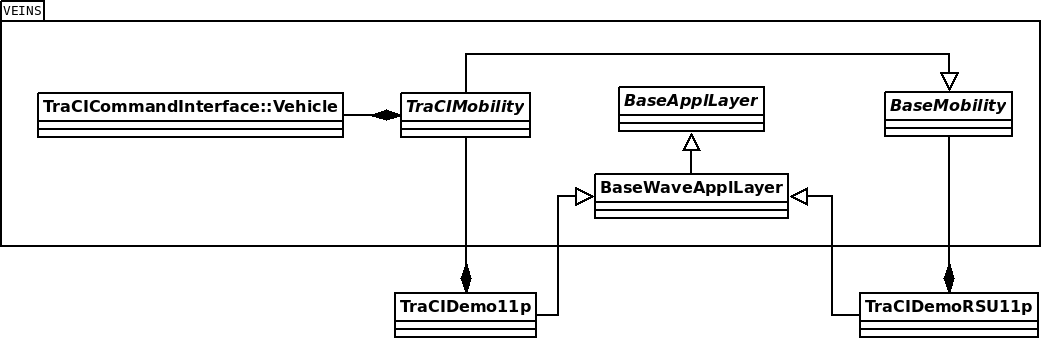
\includegraphics[scale=.43]{figuras/cap5/51ClassesVEINS}
	  \caption{\label{fig_5.1}Diagrama Simplificado de Classes do VEINS}
	 \end{figure}
	
   	\par Vale ressaltar que este diagrama de classes é uma versão simplificada do diagrama original deste \textit{framework}.
   		
	\begin{table}[H]
		\centering
        \renewcommand{\arraystretch}{1.5}
        \begin{tabular}{|p{4.4cm}|p{10.6cm}|}
			\hline
			\multicolumn{1}{|c|}{\textbf{Classes}}  & \multicolumn{1}{c|}{\textbf{Descrição}}                                                                                                                                  \\ \hline
			BaseApplLayer                  & Base para uma camada de Aplicação Genérica. Implementa o envio de pacotes para a camada inferior. \\ \hline
			BaseMobility                   & Base para todos os tipo de mobilidade para dispositivos Car2X. Esta base provê comportamento apenas para módulos estáticos como Unidades de Acostamento (RSUs). \\ \hline
			TraCIMobility                  & Classe abstrata que gerencia mobilidade dinâmica para dispositivos Car2X móveis. \\ \hline
			TraCICommandInterface\newline::Vehicle & Implementação de mobilidade para Veículos. Permite alteração de velocidade, mudança de rota, e obtenção de dados sobre a posição atual. \\ \hline
			BaseWaveApplLayer              & Base para camada de Aplicação WAVE com funcionalidades específicas como a criação, envio e recebimento de WSMs. \\ \hline
			TraCIDemo11p                   & Aplicação Exemplo para comunicação entre Veículos (OBUs). \\ \hline
			TraCIDemoRSU11p                & Aplicação Exemplo para Unidades de Acostamento (RSUs). \\ \hline
		\end{tabular}
		\caption{Descrição das Classes do VEINS}
		\label{tab_5.1}
	\end{table}
	
	\subsection{Aplicação de Emergência}
	
	\par Atualmente, os veículos de segurança pública utilizam-se apenas de giroscópio e sirene para solicitar passagem no trânsito, o que faz com que quaisquer barreiras visuais e sonoras dificultem a percepção de outros motoristas, possibilitando a análise de novos métodos de alerta que não sejam influenciados por estes aspectos.
	
	\par As Redes Veiculares permitem um novo meio de comunicação no trânsito, proporcionado uma alternativa nos momentos em que o giroscópio e sirene não são suficientes. Por ser uma tecnologia que permite a comunicação em um ambiente de trocas rápidas de informação, os veículos comuns tomam ciência antecipa de fatos ocorridos no trânsito.
	
	\par O código fonte do VEINS foi modificado, e uma aplicação de emergência foi desenvolvida para o estudo de caso neste trabalho. Esta aplicação objetiva ser de benefício para veículos de segurança pública, tais quais:
	\begin{itemize}
		\item Veículos de Socorro
		\item Veículos Policiais
		\item Veículos de Fiscalização e Operação de Trânsito
		\item Veículos de Agentes Públicos
	\end{itemize}
	
	\par Esta aplicação, quando ativada, emite mensagens periódicas aos dispositivos Car2X nas redondezas. A partir do recebimento destas mensagens, os veículos comuns podem ser orientados para uma melhor tomada de decisão no trânsito.
	
	\par Um diagrama de classes da aplicação de emergência foi desenhado e é apresentado na \autoref{fig_5.2}.
	
    \begin{figure} [H]
	    \centering
	    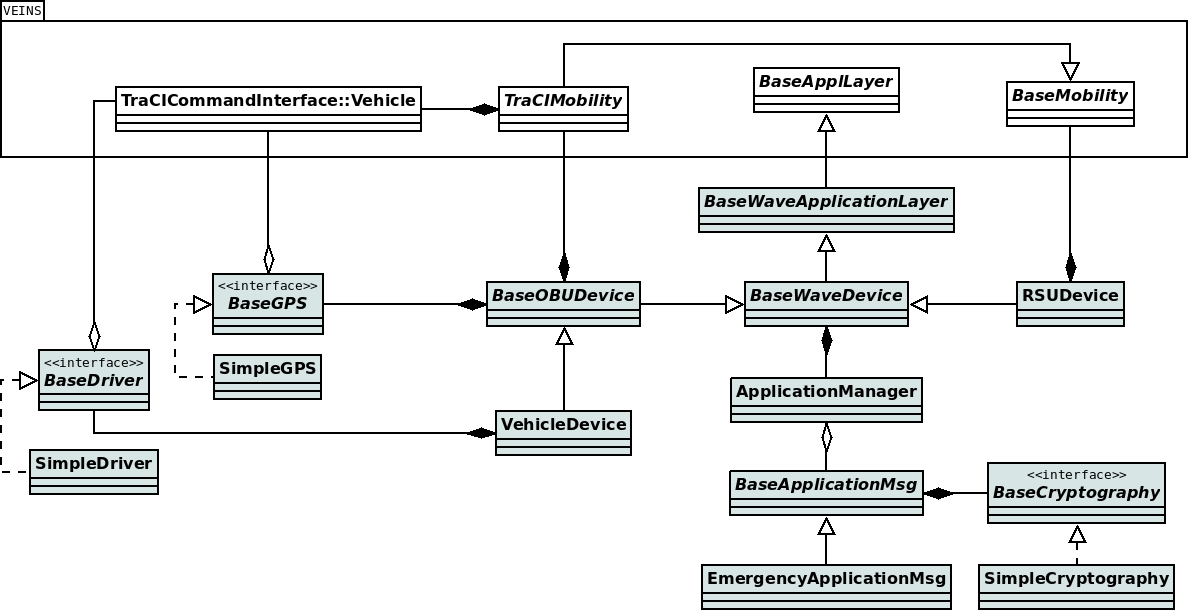
\includegraphics[scale=.37]{figuras/cap5/52ClassesEstudodeCaso}
	    \caption{\label{fig_5.2}Diagrama de Classes para o Estudo de Caso}
    \end{figure}

	A \autoref{tab_5.2} contém uma breve descrição das classes desenvolvidas para extensão do VEINS e para este estudo de caso.

    \begin{table}[H] %[?] ARRUMAR tamanho da tabela e rever italicos+negritos! OBS: REFERENCIAR LIVRO DO PADRAO DE PROJETO COMPOSITE
    	\centering
	    \renewcommand{\arraystretch}{1.4}
	    \begin{tabular}{|p{4.8cm}|p{10.2cm}|}
    		\hline
    		\multicolumn{1}{|c|}{\textbf{Classes}} & \multicolumn{1}{c|}{\textbf{Descrição}} \\ \hline
    		BaseWaveApplicationLayer, BaseWaveDevice & Classes inspiradas na classe \textit{BaseWaveApplLayer} do VEINS. Esta classe foi refatorada com intuito de simplificar o entendimento e diminuir o acoplamento do código. \\ \hline
    		BaseDriver & Interface que implementa comportamentos de um motorista. A classe concreta \textit{SimpleDriver} implementa um motorista simples com uma função simples de mudança de faixa. A base desta função foi adicionada em \textit{TraCICommandInterface::Vehicle}, a fim de possibilitar a comunicação com o simulador de tráfego. Outros tipos de motoristas com comportamentos mais complexos podem ser implementados. \\ \hline
    		BaseGPS & Interface com funções específicas de GPS. A classe concreta \textit{SimpleGPS} implementa um GPS simples com comportamentos básicos, como a obtenção e verificação de rotas de veículos. \\ \hline
    		BaseOBUDevice & Classe abstrata que contém comportamentos comuns em dispositivos Car2X móveis para veículos, como a inicialização de um GPS. A classe concreta \textit{VehicleDevice} invoca um objeto motorista. Outros tipos de dispositivos Car2X móveis podem ser implementados para pedestres e ciclistas, por exemplo. \\ \hline
    		RSUDevice & Classe utilizada por Unidades de Acostamento. Instancia um objeto \textit{BaseMobility}, característico de dispositivos estáticos. \\ \hline
    		ApplicationManager & Classe que gerencia aplicações inspirado no Padrão de Projeto Composite. O Gerente de Aplicações permite ao dispositivo WAVE executar diversas aplicações ao mesmo tempo, diferente dos exemplos do VEINS, onde cada dispositivo executa exclusivamente uma aplicação. \textit{BaseApplicationMsg} é uma classe abstrata que contém informações comuns à aplicações WAVE. É possível a adição de novas classes no futuro como aplicações de clima, comboio de veículos, segurança no tráfego, etc. \\ \hline
    		BaseCryptography & Interface que contém a base para criptografia dos dados das aplicações. A classe concreta \textit{SimpleCryptography} implementa uma criptografia simples como exemplo. \\ \hline
    		EmergencyApplicationMsg & Principal classe para o estudo de caso deste trabalho. Contém comportamentos de envio e recepção de mensagens de emergência. Requisita serviços de um GPS e contém o \textbf{PSID 0x0C}. \\ \hline
    	\end{tabular}
		   \caption{Descrição das Classes desenvolvidas}
		   \label{tab_5.2}
    \end{table}

    \par Foi escolhido o método de envio das mensagens de emergência no formato broadcast com o intuito de garantir que todos veículos na proximidade recebam o alerta. Entretanto, conforme analisado por Sommer e Dressler (2015), o envio de mensagens broadcast no meio veicular pode gerar um problema de "congestionamento de transmissões". Existem propostas de solução para o problema, porém estas não serão tratadas no trabalho.

	\par As mensagens da aplicação de emergência são enviadas no formato broadcast. Estas mensagens são de alcance direto (\textit{single-hop} ou salto único) e geradas na camada de aplicação WAVE. Serão requisitados para o envio da mensagem apenas os serviços da camadas de aplicação, da subcamada de enlace MAC e da camada física. Os serviços de outras camadas, como a de transporte e a subcamada de enlace LLC são apropriados para o envio de outras naturezas de mensagens, como mensagens de protocolos roteamento que contém múltiplos saltos (\textit{multihop}).

	\par O tamanho dos dados nas mensagens de emergência é dinâmico. Para este estudo de caso, o campo \textit{wsmData} contém o percurso parcial a ser percorrido pelo veículo de segurança pública. O formato deste campo é o seguinte:

	\begin{center} $ (L_1) [R_1] [R_2] … [R_n] $ \end{center}

	\par  $ L_1 $ e $ R_1 $ representam respectivamente a faixa e rua em trânsito. $ R_2 $ até $ R_n $ simbolizam as próximas ruas a serem percorridas pelo veículo de segurança pública. 

	\par Devido à sua natureza, a aplicação de emergência utiliza o PSID \textbf{0x0C} no cabeçalho das mensagens, apropriado para situações de emergência. O código abaixo representa como essa informação é gerada pelo veículo de segurança pública via função \textbf{prepareMessage}. % [?] verificar se é prepareMsg msm

    \begin{table}[H] %[?] Colocar cor no codigo. Fica em tabela msm? Coloca legenda ou n?
	    \centering
	    \renewcommand{\arraystretch}{1.2}
	    \begin{tabular}{|p{15cm}|}
		    \hline
		    //numberOfRoads: Número máximo de ruas a ser obtido, inicializado no construtor \\
            std::string data = gps->getCourse(\textbf{numberOfRoads}); \\
            std::string encryptedData = cryptography->encrypt(data); \\
            \\
            WaveShortMessage* wsm = new WaveShortMessage(*baseWsm); \\
            wsm->setWsmData(\textbf{encryptedData}.c\_str()); \\
            wsm->setPsid(\textbf{myPsid}); //myPsid: inicializado no construtor com valor \textbf{0x0C} \\
            wsm->setChannelNumber(Channels::\textbf{CCH}); \\
            wsm->addByteLength(encryptedData.size()); \\
            \\
            return wsm; \\
		    \hline
	    \end{tabular}
    \end{table}

    \par A aplicação de emergência solicita o percurso do veículo a um GPS (Rua Atual + próximas ruas) e encripta esta informação logo em seguida. Com o dado pronto para ser enviado, a aplicação inicia a preparação da mensagem tendo como base uma WAVE \textit{Short Message} (WSM) inicializada pela classe \textit{BaseWaveApplicationLayer}. Esta aplicação utiliza a classe \textit{BaseWaveApplicationLayer} para incluir na WSM o dado encriptado, o PSID da aplicação e o número do canal a ser utilizado, que neste caso é o canal de controle.


	\section{\label{sec:estudoDeCaso}Estudo de Caso}

	\par Para elucidação do tema proposto neste trabalho, foram criados neste estudo de caso 3 experimentos, que estão detalhados logo a seguir.

	\subsection{Descrição dos Experimentos}

	\par A aplicação de emergência descrita na seção anterior será utilizada e medida nos seguintes experimentos: 

	\begin{enumerate}
		\item Análise de comunicações entre veículos em uma rodovia simples.
		\item Análise de comunicações entre veículos e estruturas de acostamento em uma rodovia simples.
		\item Análise de comunicações entre veículos e estruturas de acostamento na microrregião de Ipanema e Copacabana no Rio de Janeiro.
	\end{enumerate}

	\par Os experimentos 1 e 2 contém simulações com cenários e métricas mais inteligíveis. Estes experimentos têm por objetivo elucidar o funcionamento das comunicações interveiculares, preparando o leitor para o experimento 3.

	\par O conjunto de experimentos 3 apresenta medições mais complexas, como a análise de valores ótimos para parâmetros da aplicação de emergência utilizados por dispositivos Car2X em tráfego rodoviário na região dos bairros de Ipanema e Copacabana, no Rio de Janeiro.

	\par Os experimentos citados serão frequentemente comparados com suas medições chamadas de “medições base”, as quais não executam a aplicação de emergência em seus cenários.

	\par Cada medição de cada experimento foi executada 100 vezes para reprodução de aleatoriedade. O SUMO estabelece uma nova posição inicial e velocidade máxima para cada veículo a cada nova repetição.

	\par É necessário o controle destas sementes aleatórias (geradas pelo SUMO) para garantir que o mesmo estado inicial seja replicado nas outras medições, como:

	\begin{itemize}
		\item Medição base (Sem comunicação)
		\item Aplicação ativa (Comunicação V2V)
		\item Aplicação ativa (Comunicação V2X)
	\end{itemize}
	
	\par O controle destas sementes permite o estudo técnico do impacto da Rede Veicular em cada cenário específico.

	\subsection{Experimentos 1 e 2: Descrição do Cenário}
	
	\par O objetivo dos experimentos 1 e 2 é mostrar o funcionamento e a efetividade da aplicação desenvolvida em comunicações interveiculares. Ambos possuem apenas função demonstrativa.
	
	\par Para a simular estes experimentos, um cenário comum foi desenvolvido por meio do software netedit, contido no pacote do \textit{framework} SUMO. Foi desenhada uma rodovia de duas pistas com faixas duplas de mesmo sentido e 4000 metros de comprimento, conforme mostrado na \autoref{fig_5.3}.
	
	 \begin{figure}[H]
	 	\centering
	 	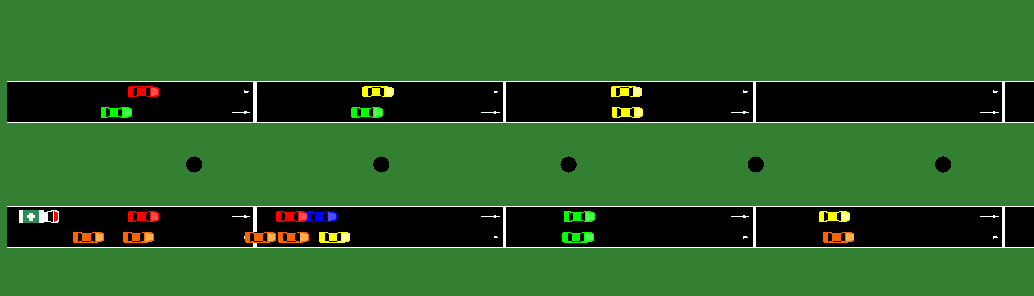
\includegraphics[scale=.355]{figuras/cap5/53CenarioExperimentos1e2}
	 	\caption{\label{fig_5.3}Cenários dos Experimentos 1 e 2 (escala reduzida)}
	 \end{figure}
	 
	 \par Neste experimento, 19 veículos e 5 unidades de acostamento localizadas entre as pistas foram espalhadas pelo cenário. O número baixo de veículos deve-se a limitações do hardware disponível para execução das simulações. A \autoref{tab_5.3} traz informações mais detalhadas sobre os dispositivos Car2X contidos neste cenário.
	 
	 \begin{table}[H]
	 	\centering
	 	\renewcommand{\arraystretch}{1.5}
	 	\begin{tabular}{|p{2.4cm}|p{3.4cm}|p{2.5cm}|p{6cm}|}
	 		\hline
	 		\textbf{Dispositivos Car2X} & \textbf{Representado(s) por} & \textbf{Potência de transmissão} & \textbf{Aplicações sendo executadas} \\ \hline
	 		secOBU{[}0{]} & Veículo de Resgate & 20 mW & Aplicação de Emergência com módulo de envio periódico de mensagens. \\ \hline
	 		OBU{[}0..18{]} & Veículos Comuns (Diversas cores) & 20 mW & Aplicação Genérica de Emergência. \\ \hline
	 		RSU{[}0..4{]} & Círculos Pretos & 30 mW & Aplicação Genérica de Emergência autorizada a replicar mensagens. \\ \hline
	 	\end{tabular}
 		\caption{Dispositivos Car2X no cenário dos experimentos 1 e 2}
 		\label{tab_5.3}
	 \end{table}
	 
	\par Nos experimentos 1 e 2, os valores dos parâmetros periodicidade do envio das mensagens e número de ruas foram definidos respectivamente como 3 segundos e 3 ruas. 
	
	\par Os veículos comuns usam uma distribuição de velocidades máximas que respeita a velocidade máxima permitida da rodovia. Neste cenário, a velocidade máxima da rodovida é de 40 m/s ou 144 km/h. Apenas o veículo de emergência pode ultrapassar o limite máximo de velocidade.
	
	\par Durante o experimento 1, as unidades de acostamento públicas permaneceram desligadas e apenas são avaliadas as mensagens trocadas entre veículos. No experimento 2, estas RSUs estão em funcionamento e replicam as mensagens recebidas pelo veículo de resgate. É válido ressaltar que a relação entre os valores de potência de transmissão e alcance do sinal são diretamente proporcionais. Portanto, as mensagens geradas por unidades de acostamento conseguem alcançar maiores distâncias se o valor da potência de transmissão for maior.
	
	\par Conceitualmente, podemos dizer que os veículos comuns que receberem a mensagem de emergência poderiam representar as informações recebidas por meio sem fio em um mapa no painel do veículo e emitir alertas sonoros em uma real situação de emergência. Estes alertas poderiam requisitar uma ação do motorista para desobstruir a passagem do veículo de segurança pública caso este esteja nos arredores, conforme mostrado em conceito na \autoref{fig_5.4}.
	
	\begin{figure}[H]
		\centering
		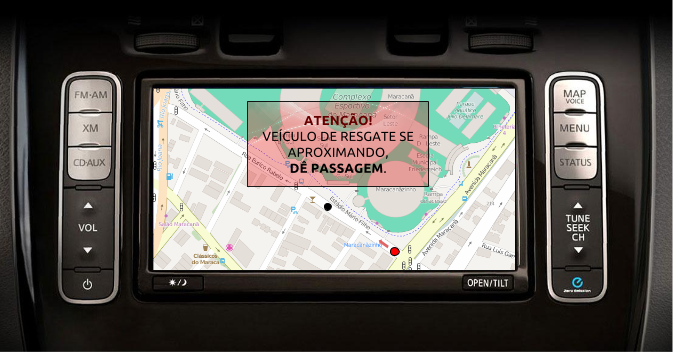
\includegraphics[scale=.65]{figuras/cap5/54ConceitoComputadorDeBordo}
		\caption{\label{fig_5.4}Computador de Bordo solicitando abertura de passagem (figura conceitual)}
	\end{figure}
	
	\subsubsection{Análise e Resultados: Experimento 1}
	
	\par O experimento 1 mede a influência da aplicação de emergência em comunicações de veículo para veículo no cenário proposto. Cada medição foi executada 100 vezes para reprodução de aleatoriedade e para posterior coleta e análise estatística.
	
	\par Durante a simulação, pode-se perceber que as mensagens de broadcast do veículo de resgate alcançam também veículos comuns que estão em ruas paralelas, ou seja, fora de sua rota de colisão. Estes veículos recebem a mensagem porém não realizam qualquer ação, visto que estão em percursos diferentes em relação ao veículo de resgate. Isto é representado na \autoref{fig_5.5} e na \autoref{fig_5.6}.
	
	\begin{figure}[H]
		\centering
		\includegraphics[scale=.9]{figuras/cap5/55Experimento1TkEnv}
		\caption{\label{fig_5.5}Veículo de Resgate envia mensagem de broadcast}
	\end{figure}
	
	\begin{figure}[H]
		\centering
		\includegraphics[scale=.35]{figuras/cap5/56Experimento1SUMO}
		\caption{\label{fig_5.6}Apenas os veículos da pista inferior mudam de faixa após mensagem}
	\end{figure}
	
	\par Os veículos que estão em rota de colisão com o veículo de resgate procuram o momento e espaço mais seguros para mudarem de faixa. Algumas ações são tomadas pelos motoristas destes veículos para evitar ao máximo o bloqueio da passagem. A \autoref{fig_5.7} mostra que no momento em que a mensagem de emergência alcança o veículo azul este está em menor velocidade em relação ao veículo vermelho. A mudança de faixa não pode ser realizada imediatamente após o recebimento da mensagem devido a uma possível colisão. 
	
	\begin{figure}[H]
		\centering
		\includegraphics[scale=.4]{figuras/cap5/57Experimento1SUMO2}
		\caption{\label{fig_5.7} Veículo azul em menor velocidade porém não é seguro mudar de faixa}
	\end{figure}
	
	\par Após alguns instantes, o veículo azul muda de faixa quando encontra uma distância segura para o veículo vermelho (\autoref{fig_5.8}).
	
	\begin{figure}[H]
		\centering
		\includegraphics[scale=.35]{figuras/cap5/58Experimento1SUMO3}
		\caption{\label{fig_5.8} Após alguns instantes a mudança de faixa é realizada}
	\end{figure}
	
	\par Outra situação observada no experimento 1 é vista na \autoref{fig_5.9}. Embora em maior velocidade, o veículo vermelho é influenciado pela mensagem de emergência e não realiza a ultrapassagem a fim de não bloquear a rota do veículo de resgate.
	
	\begin{figure}[H]
		\centering
		\includegraphics[scale=.4]{figuras/cap5/59Experimento1SUMO4}
		\caption{\label{fig_5.9}Veículo vermelho é influenciado pela mensagem de emergência}
	\end{figure}
	
	\par O veículo vermelho, que após sofrer a ultrapassagem e não estar mais na rota de colisão do veículo de resgate, pode ultrapassar o veículo amarelo no momento em que encontra uma distância segura para a ação. A \autoref{fig_5.10} apresenta o momento deste acontecimento.
	
	\begin{figure}[H]
		\centering
		\includegraphics[scale=.5]{figuras/cap5/510Experimento1SUMO5}
		\caption{\label{fig_5.10}Veículo vermelho muda de faixa e realiza a ultrapassagem}
	\end{figure}
		
	\par A \autoref{tab_5.4} apresenta o tempo total de trajeto pelo veículo de resgate no experimento 1. O endereço para as tabelas que contém todos os valores da amostra está no \autoref{links}.
		
	\begin{table}[H]
		\centering
		\renewcommand{\arraystretch}{1.5}
		\begin{tabular}{|l|c|c|}
			\hline
			\multicolumn{1}{|c|}{\textbf{Métricas}} & \textbf{Medição base} & \textbf{Aplicação de emergência} \\ \hline
			Total percorrido & 4000 m & 4000 m \\ \hline
			Tempo total gasto & 128.62 s & 120.82 s \\ \hline
			Velocidade média & 111,95 km/h & 119,18 km/h \\ \hline
		\end{tabular}
		\caption{Resultados Experimento 1}
		\label{tab_5.4}
	\end{table}
	
	\par É possível notar que devido a utilização da aplicação de emergência no cenário proposto, o veículo de resgate manteve uma velocidade média maior e pode reduzir o tempo total do trajeto em 6,07\%.
	
	\subsubsection{Análise e Resultados: Experimento 2}
	
	\par O experimento 2 mede a influência da aplicação de emergência em comunicações entre veículos e unidades de acostamento no cenário proposto. Cada medição foi executada 100 vezes para reprodução de aleatoriedade e para posterior coleta e análise estatística.
	
	\par Por ter uma potência de transmissão maior, as unidades de acostamento podem alcançar maiores distâncias do que as unidades de bordo. A \autoref{fig_5.11} apresenta o raio máximo de alcance de cada RSU no cenário proposto. Cada RSU está no raio de alcance de outra unidade de bordo subsequente.
	
	\begin{figure}[H]
		\centering
		\includegraphics[scale=.42]{figuras/cap5/511Experimento2TkEnv}
		\caption{\label{fig_5.11}Raio de alcance das RSUs}
	\end{figure}
	
	\par A utilização de unidades de acostamento públicas é de relevante vantagem para a aplicação de emergência visto que sua mensagem alcança mais rapidamente um número maior de veículos comuns, permitindo a estes uma preparação mais antecipada à aproximação de algum veículo de segurança pública. Como exemplo, vemos na \autoref{fig_5.12} que aproximadamente aos 14 segundos da simulação todos os veículos num raio de 4 quilômetros já haviam recebido a mensagem da aplicação de emergência no experimento 2, enquanto apenas 5 veículos haviam recebido a mensagem de emergência no experimento 1.
	
	\begin{figure}[H]
		\centering
		\includegraphics[scale=.4]{figuras/cap5/512Experimento2TkEnv2}
		\caption{\label{fig_5.12}Experimentos 1 e 2 - Comparação do tempo de recebimento das mensagens}
	\end{figure}	
	
	\par A \autoref{tab_5.5} apresenta o tempo total de trajeto pelo veículo de resgate no experimento 2. O endereço para as tabelas contendo todos os valores da amostra estão no \autoref{links}.
	
	\begin{table}[H]
		\centering
		\renewcommand{\arraystretch}{1.5}
		\begin{tabular}{|l|c|p{5.2cm}|}
			\hline
			\multicolumn{1}{|c|}{\textbf{Métricas}} & \textbf{Medição base} & \textbf{Aplicação  de emergência executada com RSUs} \\ \hline
			Total percorrido & 4000 m & \multicolumn{1}{c|}{4000 m} \\ \hline
			Tempo total gasto & 128.62 s & \multicolumn{1}{c|}{120,68 s} \\ \hline
			Velocidade média & 111,95 km/h & \multicolumn{1}{c|}{119,2 km/h} \\ \hline
		\end{tabular}
		\caption{Resultados Experimento 2}
		\label{tab_5.5}
	\end{table}
	
	\par Nota-se que a utilização da aplicação de emergência e das unidades de acostamento públicas no cenário proposto fez o veículo de resgate manter uma velocidade média maior em relação ao experimentos 1, reduzindo o tempo total de trajeto do veículo de resgate em 6,17\% em relação à medição base.
	
	
	\subsection{Experimento 3: Aplicação de Emergência na região de Ipanema-Copacabana}
	
	\par Para o terceiro cenário, um cenário mais complexo foi desenvolvido para a realização de experimentos. Foi importado o mapa do entorno da região de Ipanema-Copabana na cidade do Rio de Janeiro por meio do site do \textit{OpenStreetMap}. Esta região foi escolhida por serem dois bairros turísticos mundialmente famosos da cidade do Rio de Janeiro,  além do fato deles também possuírem condições propícias à simulações de tráfego, como melhor planejamento urbano, número relevante de faixas por vias, semáforos, obstáculos, etc.
	
	\par A \autoref{fig_5.13} apresenta o percurso do veículo de resgate, que parte da Avenida Vieira Souto em Ipanema e segue para Copacabana via Avenida Nossa Senhora de Copacabana até seu ponto de destino. São percorridos aproximadamente 4800 metros neste trajeto, representado na imagem pela linha vermelha. Devido ao comportamento apresentado pelas unidades de acostamento no segundo experimento, 7 RSUs (pontos pretos \autoref{fig_5.13}) foram espalhadas para auxiliar na propagação das mensagens da aplicação de emergência. 
	
	\begin{figure}[H]
		\centering
		\includegraphics[scale=.5]{figuras/cap5/513Cenario3}
		\caption{\label{fig_5.13}Trajetória do veículo de resgate e RSUs}
	\end{figure}	
	
	\par O volume de veículos gerado para as avenidas Vieira Souto e Nossa Senhora de Copacabana foi baseado em informações de tráfego obtidos em documento da Companhia de Engenharia de Tráfego do Rio de Janeiro (CET-Rio, 2014). A \autoref{tab_5.6} apresenta os dispositivos WAVE contidos no experimento.
	
	\begin{table}[H]
		\centering
		\renewcommand{\arraystretch}{1.5}
		\begin{tabular}{|p{2.4cm}|p{3.65cm}|p{2.5cm}|p{6cm}|}
			\hline
			\textbf{Dispositivos Car2X} & \textbf{Representado por} & \textbf{Potência de transmissão} & \textbf{Aplicações sendo executadas} \\ \hline
			secOBU{[}0{]} & Veículo de Resgate & 20 mW & Aplicação de Emergência com módulo de envio periódico de mensagens. \\ \hline
			OBU{[}0..114{]} & Veículo de diversas cores & 20 mW & Aplicação Genérica de Emergência. \\ \hline
			RSU{[}0..6{]} & Pontos Pretos & 30 mW & Aplicação Genérica de Emergência autorizada a replicar mensagens. \\ \hline
		\end{tabular}
		\caption{Dispositivos Car2X no cenário dos experimento 3}
		\label{tab_5.6}
	\end{table}
	
	\par Neste experimento foram incorporados modelos de atenuação de sinal por perda de caminho e reflexão (\textit{TwoRayInterferenceModel}) e por obstáculos (\textit{SimpleObstacleShadowing}) do framework VEINS para geração de dados mais próximos à realidade. Na \autoref{fig_5.14} são mostrados os raios de alcance de sinal das unidades de bordo contidas neste cenário. Cada RSU está no raio de alcance de outra unidade de acostamento subsequente.
	
	\begin{figure}[H]
		\centering
		\includegraphics[scale=.4]{figuras/cap5/514Cenario3TkEnv}
		\caption{\label{fig_5.14}Disposição das RSUs no Experimento 3}
	\end{figure}	
	
	\par Foi estabelecida uma distribuição dos valores de velocidade máxima dos veículos comuns, sendo inferiores ao de velocida máxima permitida em cada trecho (variam entre 60 e 100 km/h). Apenas o veículo de segurança pública pode ultrapassar o limite máximo de cada trecho pois precisa percorrer o trajeto descrito no menor tempo possível.

	\par A \autoref{fig_5.15} mostra uma parte do cenário Ipanema-Copacabana no SUMO-GUI. É necessário ressaltar que para este cenário todos os semáforos das ruas percorridas pelo veículo de resgate estão em funcionamento.

	\begin{figure}[H]
		\centering
		\includegraphics[scale=.34]{figuras/cap5/515Cenario3SUMO}
		\caption{\label{fig_5.15}Fluxo dos Carros e obstáculos em vermelho no  Experimento 3}
	\end{figure}
	
	\par Os dados coletados no experimento 3 tiveram seus \textit{outliers} filtrados. Um \textit{outlier} é descrito em estatística como um ponto que está muito distante das demais observações em uma série. Comumente é chamado de “ponto fora da curva”. A utilização da análise de \textit{outliers} otimiza análises e garante confiabilidade na amostra.
	
	\par O experimento tratado terá 95\% de confiabilidade, isto é, serão analisados os 95\% dos valores que encontram-se entre a média somada a duas vezes o desvio padrão e a média subtraída de duas vezes o desvio padrão.
	
	\subsubsection{Análise e Resultados: Experimento 3}
	
	\par Num conjunto de experimentos preliminar, foram medidos os parâmetros periodicidade e número de ruas da aplicação de emergência com o objetivo de encontrar seu valor ótimo para cenário Ipanema-Copacabana. Para o número de ruas, foi estabelecido um conjunto limitado de valores {2, 3, 4, 5}. Já o parâmetro periodicidade detém um conjunto de valores {0.5, 1.0, 1.5, 2.0, 2.5} medidos em segundos. 
	
	\par Descobriu-se que os valores ótimos dos parâmetros para o cenário em questão são de 0,5 segundo de periodicidade e 4 ruas de abrangência. O endereço para as tabelas contendo todos os valores das amostras está no \autoref{links}. Vale ressaltar que estes valores não serão necessariamente ótimos para outros cenários. É necessário um estudo aprofundado para obtenção de valores ótimos que possam ser utilizados em quaisquer situações.
	
	\par Os conjuntos de experimentos compartilham o mesmo conjunto de sementes aleatórias em cada medição, inclusive a medição base. Cada medição foi executada 100 vezes para reprodução de aleatoriedade e para posterior coleta e análise estatística.
	
	\par O comportamento da aplicação de emergência em unidades de bordo e de acostamento ocorre conforme discutido nos experimentos 1 e 2. As unidades de bordo de veículos comuns continuam apenas recebendo as mensagens de emergência enquanto as unidades de acostamento públicas podem receber e replicar as mensagens de emergência provenientes do veículo de resgate.
	
	\par Na medição base, onde são mensurados os dados de cenários que não utilizam a aplicação de emergência, verificou-se que a média de tempo total de trajeto do veículo de resgate é de 471,53 segundos. O gráfico na \autoref{fig_5.16} evidencia os valores medidos além de identificar os \textit{outliers} nos círculos vermelhos.
	
	\begin{figure} [H]
		\centering
		\includegraphics[scale=.4]{figuras/cap5/516Grafico1}
		\caption{\label{fig_5.16}Gráfico de Medição Base - \textit{Outliers} nos círculos vermelhos}
	\end{figure}
	
	Os valores coletados da medição base do cenário em questão estão dispostos na \autoref{tab_5.7}.
	
	\begin{table}[H]
		\centering
		\renewcommand{\arraystretch}{1.5}
		\begin{tabular}{|l|c|}
			\hline
			\multicolumn{1}{|c|}{\textbf{Métricas}} & \textbf{Medição base (semáforos habilitados)} \\ \hline
			Total percorrido & 4800 m \\ \hline
			Média de tempo total & 477,11 s \\ \hline
			Média após Análise de Outliers & 471,53 s \\ \hline
			Velocidade média & 36,65 km/h \\ \hline
		\end{tabular}
		\caption{Resultados do Experimento 3 - Medição base}
		\label{tab_5.7}
	\end{table}
	
	\par A segunda medição faz uso da aplicação de emergência. Com a utilização desta, verificou-se que a média de tempo total de trajeto do veículo de resgate é de 452,25 segundos. O gráfico contido na \autoref{fig_5.17} evidencia os valores medidos além de identificar os \textit{outliers}.
	
	\begin{figure} [H]
		\centering
		\includegraphics[scale=.4]{figuras/cap5/517Grafico2}
		\caption{\label{fig_5.17}Gráfico de Aplicação de Emergência ativada - \textit{Outliers} nos círculos vermelhos}
	\end{figure}
	
	Os valores coletados da medição com a utilização da aplicação de emergência estão dispostos na \autoref{tab_5.8}.
	
	\begin{table}[H]
		\centering
		\renewcommand{\arraystretch}{1.5}
		\begin{tabular}{|l|c|}
			\hline
			\multicolumn{1}{|c|}{\textbf{Métricas}} & \textbf{Medição base (semáforos habilitados)} \\ \hline
			Total percorrido & 4800 m \\ \hline
			Média de tempo total & 458,06 s \\ \hline
			Média após Análise de Outliers & 452,25 s \\ \hline
			Velocidade média & 38,21 km/h \\ \hline
		\end{tabular}
		\caption{Resultados do Experimento 3 - Medição com aplicação ativada}
		\label{tab_5.8}
	\end{table}
	
	\par Tais resultados apresentaram o veículo de resgate com uma rapidez de 4,09\% quando a aplicação de emergência está em uso.
	
	\par Durante a simulação, pode-se perceber uma “limitação” que não reproduz a realidade: O veículo de resgate respeitava completamente o tempo dos semáforos. Entretanto, o próprio código brasileiro de trânsito permite que os veículos de resgate avance o sinal vermelho do semáforo. Na prática, este veículo diminuiria sua velocidade e forçaria o avanço do sinal, desde que este ato pudesse ser realizado de forma segura.
	
	\par Desta forma, a fim de executar uma análise mais crítica do experimento 3, consideramos um cenário ótimo onde os semáforos sempre estariam abertos na aproximação do veículo de resgate. Este cenário foi imaginado com o intuito de avaliar o tempo de resposta do veículo caso este não ficasse preso nos semáforos. A \autoref{fig_5.18} apresenta o gráfico com os resultados obtidos.
	
	\begin{figure}[H]
		\centering
		\includegraphics[scale=.4]{figuras/cap5/518Grafico3}
		\caption{\label{fig_5.18}Gráfico de Aplicação de Emergência ativada em cenário com semáforos abertos - \textit{Outliers} nos círculos vermelhos}
	\end{figure}
	
	Os valores coletados da medição com a utilização da aplicação de emergência e os semáforos abertos estão dispostos na \autoref{tab_5.9}.
	
	\begin{table}[H]
		\centering
		\renewcommand{\arraystretch}{1.5}
		\begin{tabular}{|l|c|}
			\hline
			\multicolumn{1}{|c|}{\textbf{Métricas}} & \textbf{Medição base (semáforos habilitados)} \\ \hline
			Total percorrido & 4800 m \\ \hline
			Média de tempo total & 304,12 s \\ \hline
			Média após Análise de Outliers & 303,53 s \\ \hline
			Velocidade média & 56,93 km/h \\ \hline
		\end{tabular}
		\caption{Resultados - Medição com aplicação ativada e semáforos abertos}
		\label{tab_5.9}
	\end{table}

	\par Analisando as medições com semáforos habilitados e desabilitados, podemos verificar que o uso da aplicação de emergência somado aos semáforos abertos resultou em uma rapidez de 35,63\% no tempo total de percurso do veículo de resgate. Este cenário foi imaginado para avaliar uma situação mais próxima da realidade, onde os veículos de resgate avançam os sinais vermelhos.

	\section{Resultados e Discussões}

	\par Podemos perceber uma melhora nos tempos totais de trajeto do veículo de resgate em todos os cenários. A performance da aplicação de emergência poderia trazer resultados ainda mais significativos caso algumas limitações do software de simulação de tráfego fossem minimizadas.
	
	\par No caso do software de simulação de tráfego SUMO, algumas destas limitações foram percebidas no curso deste estudo de caso, como por exemplo:
	
	\begin{enumerate}
		\item Não é permitida a ultrapassagem de semáforos fechados por quaisquer grupos de veículos. Esta situação, possível na vida real, é utilizada por alguns veículos de segurança pública caso estes estejam em serviço;
		\item Não é atualmente implementada no SUMO a possibilidade de veículos percorrerem lado a lado em mesma faixa. Exemplo: Moto ultrapassa veículo comum sem mudar de faixa, percorrendo o trajeto ao lado deste veículo, mantendo uma distância segura;
		\item Não é permitido atualmente no SUMO um veículo permanecer posicionado no meio de duas faixas. Esta manobra é muito usada pelos veículos de resgate, quando dois veículos que ocupam duas faixas vão para os extremos opostos de cada uma destas faixas para desobstrução de passagem;
		\item No SUMO, os veículos não aceleram ou desaceleram antes de realizar a troca de faixa, ocasionando uma demora na ultrapassagem de veículos;
		\item Não é permitido atualmente no SUMO um veículo realizar uma passagem pela contramão ou pela calçada, como é comumente visto em situações reais. 
	\end{enumerate}
	
	\par As limitações citadas influenciam a métrica de tempo total do veículo de resgate nos experimentos, ainda que a aplicação de emergência tenha ocasionado efeitos percebidos como  melhor fluidez do trânsito gerando um tempo total menor. A \autoref{tab_5.10} apresenta os resultados dos experimentos do estudo de caso deste trabalho.
	
	\begin{table}[H]
		\centering
		\renewcommand{\arraystretch}{1.5}
		\begin{tabular}{|p{3.5cm}|p{3.0cm}|p{3.1cm}|p{4.0cm}|}
			\hline
			\textbf{Veículo de \newline Resgate} & \textbf{Tempo Total} (Medição Base) & \textbf{Tempo Total} \newline (Aplicação de Emergência) & \textbf{rapidez em relação \newline à medição base} (\%) \\ \hline
			Experimento 1 & 128,62 s & 120,82 s & 6,07\% \\ \hline
			Experimento 2 & 128,62 s & 120,68 s & 6,17\% \\ \hline
			Experimento 3 \newline (semáforos ligados) & 471,53 s & 452,25 s & 4,09\% \\ \hline
			Experimento 3 \newline (semáforos abertos) & 471,53 s & 303,53 s & 35,63\% \\ \hline
		\end{tabular}
		\caption{Resultados Experimentos do Estudo de Caso}
		\label{tab_5.10}
	\end{table}

	\par Concluímos que a utilização de redes veiculares como um novo meio de comunicação no trânsito seria de relevante uso em eventuais desobstruções para veículos de segurança pública. Os resultados obtidos neste estudo de caso já demonstram que a utilização de mensagens de uma aplicação de emergência por intermédio de Redes Veiculares resultam em uma melhor fluidez no percurso dos veículos de resgate, de veículos policiais ou do corpo de bombeiros. Além do mais, cabe sempre ressaltar que qualquer ganho de tempo em um situação de resgate pode significar o ganho de uma vida.

	\par As unidades de acostamento seriam de grande auxílio tanto para o bem público quanto na expansão do alcance de mensagens em Redes Veiculares. 

	\par Para a realização de simulações em redes veiculares, os softwares abertos de simulação de tráfego como o SUMO ainda necessitam de ajustes para atuar de forma fidedigna ao caráter real de sua atuação. Algumas melhorias que corrigem as limitações citadas já estão previstas pela equipe de desenvolvimento do SUMO{\footnote{\href{http://sumo.dlr.de/trac.wsgi/roadmap}{http://sumo.dlr.de/trac.wsgi/roadmap} (acesso em 19 de set. 2016)}}.
	
	\par No mais, as simulações de redes veiculares auxiliam relevantemente na preparação de provas de conceito, cooperando para uma abordagem analítica de cenários e para a economia de recursos.

	%----------------------------------------------------------------
	% ---
	% Finaliza a parte no bookmark do PDF, para que se inicie o bookmark na raiz
	% ---
	\bookmarksetup{startatroot}% 
	% ---

	% ---
	% Conclusão
	% ---

% ----------------------------------------------------------
	\chapter[Conclusão]{Conclusão}

	\par A padronização da tecnologia mediante as normas IEEE 1609 e ETSI mostra uma tentativa de incentivar a adoção de Rede Veiculares pelas indústrias. Tecnologias padronizadas facilitam a produção e implantação em maior escala.

	\par A tecnologia Car2X não se apresenta apenas como futuro promissor e sim como uma realidade iminente. Nos últimos anos, inúmeras empresas de tecnologia voltaram sua atenção para a indústria automobilística a fim de desenvolver produtos com o objetivo de alcançar a tão desejada condução autônoma. CEOs de empresas automotivas argumenta que a inclusão de tecnologias eletrônicas e de comunicação sem fio em veículos é a tendência atual desta indústria{\footnote{\href{http://telematicsnews.info/2016/06/20/toyota-connected-ceo-wants-to-contextualise-connected-cars-ju7204/}{http://telematicsnews.info/2016/06/20/toyota-connected-ceo-wants-to-contextualise-connected-cars-ju7204/} (acesso em 23 de set. 2016)}.

	\par No contexto das comunicações interveiculares, há um mercado promissor para empresas de desenvolvimento de software. Aplicativos para sensores, segurança, comunicação, entretenimento, informação, controle de tráfego poderão surgir, melhorando a experiência, segurança e a comodidade dentro do veículo.

	\par No estudo de caso foi apresentado que uma aplicação de emergência alinhada à tecnologia Car2X tem o potencial de facilitar o trajeto de veículos de segurança pública. Estes veículos passam a contar com uma nova forma de sinalização de sua presença, vencendo barreiras visuais e sonoras por intermédio da replicação de suas mensagens via Rede Veicular.

% ----------------------------------------------------------

	\chapter*[Trabalhos Futuros]{Trabalhos Futuros}
	\addcontentsline{toc}{chapter}{TRABALHOS FUTUROS}

	\par O código desenvolvido para a aplicação de emergência apresentada no estudo de caso deste trabalho permite ser incrementado em trabalhos futuros. Um mecanismo simples de criptografia foi utilizado como exemplo para realizar a encriptação dos dados da mensagem de emergência. Através da biblioteca crypto++, técnicas de criptografia podem ser incluídas para novos estudos de caso.

	\par Atualmente, o código da aplicação contém orientação de mudança de faixa no corpo da mensagem de emergência. Novas orientações podem ser incluídas em trabalhos posteriores objetivando novos cenários. Como exemplo, mensagens contendo novas orientações como desaceleração, estacionamento, permissão de ultrapassagem, direção cautelosa, velocidades máxima e mínima podem ser criadas para cenários com outros fins. Novos estudos de caso poderiam simular a troca de mensagens em perseguições policiais, passagens de comitivas especiais, operações de blitz, sinalização vertical de vias, cruzamentos de tráfego intermodais (automóveis e trens, por exemplo), entre outros.

	\par Semáforos inteligentes podem ser controlados para a liberação de vias de acordo com o tráfego. É possível desenvolver aplicações para comunicação entre veículos de segurança pública e semáforos para que haja uma mudança no sincronismo dos sinais garantindo fluxo livre perto da aproximação destes.

	\par A classe Driver permite controlar ações típicas de um motorista humano no veículo. Esta poderia ser incrementada utilizando princípios de inteligência artificial. Como exemplo, as mudanças de faixa poderiam ser realizadas ou não após o raciocínio de sinapses que calculam variáveis como distância entre veículos (frontal, traseira e lateral), aceleração e condições da pista.

	\par Aplicações que comuniquem-se com semáforos possibilitariam melhor fluidez para os veículos de segurança pública caso estes pudessem alterar momentaneamente o sincronismo entre as fases do semáfaro por meio da troca de mensagens de emergência.

	\par Placas indicativas de velocidade máxima espalhadas em pontos estratégicos de uma rodovia poderiam ser equipadas de unidades de acostamento com o intuito de enviar WSMs periódicos indicando a velocidade adequada. Os dispositivos recebedores poderiam interpretar estas mensagens de diversas maneiras.

	\par Radares poderiam ser equipados com RSUs para um registro mais confiável dos veículos que não estiverem em conformidade com as leis de trânsito, enviando a multa diretamente para o dono do veículo transgressor sem depender apenas de fotos, que por vezes não são suficientes.

	\par Estudos na manipulação física do envio de mensagens WAVE podem auxiliar na diminuição de congestionamento de sinal em rodovias movimentadas. É possível diminuir ainda mais essa inundação controlando a replicação das mensagens, seja por meio da limitação do tempo de vida dos pacotes ou com a utilização de quadros de gerenciamento para o envio \textit{multicast}.

% ----------------------------------------------------------
	% ELEMENTOS PÓS-TEXTUAIS
	% ----------------------------------------------------------
	\postextual


	% ----------------------------------------------------------
	% Referências bibliográficas
	% ----------------------------------------------------------
	\newpage
	\chapter*[Referências]{Referências}
	\addcontentsline{toc}{chapter}{REFERÊNCIAS}
	\flushleft

	\begin{itemize}[label={}] %\itemsep -4pt
		
		\item HARVEY, D. The Condition of Postmodernity: An Enquiry into the Origins of Cultural Change. Wiley-Blackwell, 1992. 392 p.
		
		\item WORLD HEALTH ORGANIZATION. Global Status Report on Road Safety, 2015. Relatório. Disponível em: \url{http://www.who.int/violence_injury_prevention/road_safety_status/2015/en/}. Acesso em: 2 de maio 2016. %[?]

		\item GAST, M. S. 802.11 Wireless Networks: The Definitive Guide. Segunda Edição. O'Reilly Media, 2005. 672 p.
		
		\item DUBUISSON, O. ASN.1 Communication between Heterogeneous Systems. Morgan Kaufmann, 2001. 562 p.
		
		\item FOROUZAN, B. A.; FEGAN, S. C. Data Communications and Networking. Quarta Edição. McGraw-Hill Higher Education, 2007. 1134p. (McGraw-Hill Forouzan Networking Series)
		
		\item DELGROSSI, L.; ZHANG, T. Vehicle Safety Communications: Protocols, Security, and Privacy. Nova Jérsia: Wiley, 2012. 372 p. (Information and Communication Technology Series)
		
		\item HARTENSTEIN, H.; LABERTEAUX, K. P. VANET: Vehicular Applications and Inter-Networking Technologies. Chichester: Wiley, 2010. 435 p. (Intelligent transportation systems)
		
		\item OLARIU, S.; WEIGLE, M. A. C. Vehicular Networks: From Theory to Practice. CRC Press, 2009. 472 p. (Chapman \& Hall/CRC Computer and Information Science Series)
		
		\item BANKS, J. Discrete-Event System Simulation. Quarta Edição. Pearson Prentice Hall, 2005. 608 p. (Prentice-Hall international series in industrial and systems engineering)
		
		\item GIORDANO, S.; STOJMENOVIC, I. Position Based Routing Algorithms for Ad Hoc Networks: A Taxonomy. In: CHENG, X.; HUANG, X.; DU, D.-Z. (Eds.). Ad Hoc Wireless Networking. Kluwer Academic, 2003. p. 103-136.
		
		\item ROYER, E. M.; TOH, C.-K. A Review of Current Routing Protocols for Ad Hoc Mobile Wireless Networks. IEEE Personal Communications, v. 6, n. 2, p. 46-55, 1999.
		
		\item CHENG, J., et al. Routing in Internet of Vehicles: A Review. IEEE Transactions on Intelligent Transportation Systems, v. 16, n. 5, p. 2339-2352, 2015.
		
		\item SOMMER, C.; GERMAN, R.; DRESSLER, F. Bidirectionally Coupled Network and Road Traffic Simulation for Improved IVC Analysis. IEEE Transactions on Mobile Computing, v. 10, n. 1, p. 3-15, 2011.
		
		\item CHENG, L., et al. Multi-Path Propagation Measurements for Vehicular Networks at 5.9 GHz. In: WIRELESS COMMUNICATIONS AND NETWORKING CONFERENCE, 2008, Las Vegas.
		
		\item YANG, F., et al. An Overview of Internet of Vehicles. China Communications, v.11, n. 10, p. 1-15, 2014.
		
		\item PEGDEN, C. D.; SADOWSKI, R. P.; SHANNON, R. E. Introduction to Simulation Using Siman. Segunda Edição. McGraw-Hill, 1995. 660 p. (Industrial engineering series)
		
		\item PURSULA, M. Simulation of Traffic Systems: An Overview. Disponível em: \url{http://publish.uwo.ca/~jmalczew/gida\_5/Pursula/Pursula.html}. Acesso em: 6 de jun. 2016.
		
		\item KRAJZEWICZ, D., et al. Recent Development and Applications of SUMO: Simulation of Urban MObility. International Journal On Advances in Systems and Measurements, v. 5, n. 3-4, p. 128-138, 2012.
		
		\item JAKOB, E. Lane-Changing Model in SUMO. Proceedings of the SUMO2014 Modeling Mobility with Open Data, Berlim, v. 24, p. 77-88, 2014.
		
		\item OMNeT++ Discrete Event Simulator: What is OMNeT++. Disponível em: \url{https://omnetpp.org/intro/what-is-omnet}. Acesso em: 6 de jun. 2016.
		
		\item Documentation: Veins. Disponível em: \url{http://veins.car2x.org/documentation/}. Acesso em: 6 de jun. 2016.
		
		\item GDAL: GDAL - Geospatial Data Abstraction Library. Disponível em: \url{http://www.gdal.org/}. Acesso em: 7 de jun. 2016.
		
		\item OSGeo.org: Your Open Source Compass. Disponível em: \url{http://www.osgeo.org/}. Acesso em: 7 de jun. 2016.
		
		\item Fox-toolkit.org. Disponível em: \url{http://www.fox-toolkit.org/}. Acesso em: 7 de jun. 2016.
		
		\item Proj.4: proj.4 4.9.3 documentation. Disponível em: \url{http://proj4.org/}. Acesso em: 7 de jun. 2016.
		
		\item Xerces-C++ XML Parser. Disponível em: \url{http://xerces.apache.org/xerces-c/}. Acesso em: 7 de jun. 2016.
		
		\item VARGA, A. OMNeT++ Installation Guide: Version 5.0. Disponível em: \url{https://omnetpp.org/doc/omnetpp/InstallGuide.pdf}. Acesso em: 7 de jun. 2016.
		
		\item Tutorial: Veins. Disponível em: \url{http://veins.car2x.org/tutorial/}. Acesso em: 7 de jun. 2016.
		
		\item Installing: Sumo. Disponível em: \url{http://sumo.dlr.de/wiki/Installing}. Acesso em: 7 de jun. 2016.
		
		\item ANATEL. Plano de Atribuição, Destinação e Distribuição de Faixas de Frequências no Brasil: Ato n. 2099. Brasil, 2012. 175 p.
		
		\item IEEE COMPUTER SOCIETY. Wireless LAN Medium Access Control (MAC) and Physical Layer (PHY) Specifications: Part 11, 802.11-2012. Nova York, 2012. 2793 p.
		
		\item IEEE COMPUTER SOCIETY. IEEE Guide for Wireless Access in Vehicular Environments (WAVE): Architecture, 1609.0-2013. Nova York, 2013. 78 p.
		
		\item IEEE COMPUTER SOCIETY. IEEE Standard for Wireless Access in Vehicular Environments: Security Services for Applications and Management Messages, 1609.2-2016. Nova York, 2016. 240 p.
		
		\item IEEE COMPUTER SOCIETY. IEEE Standard for Wireless Access in Vehicular Environments (WAVE): Networking Services, 1609.3-2016. Nova York, 2016. 160 p.
		
		\item IEEE COMPUTER SOCIETY. IEEE Standard for Wireless Access in Vehicular Environments (WAVE): Multi-Channel Operation, 1609.4-2016. Nova York, 2016. 94 p.
		
		\item IEEE COMPUTER SOCIETY. IEEE Standard for Wireless Access in Vehicular Environments (WAVE): Over-the-Air Electronic Payment Data Exchange Protocol for Intelligent Transportation Systems (ITS), 1609.11-2010. Nova York, 2010. 62 p.
		
		\item IEEE COMPUTER SOCIETY. IEEE Standard for Wireless Access in Vehicular Environments (WAVE): Identifier Allocations, 1609.12-2016. Nova York, 2016. 21 p.
		
		\item IEEE COMPUTER SOCIETY. Standard for Wireless Access in Vehicular Environments: Security Services for Applications and Management Messages Amendment - Certificate Management, P1609.2a. Nova York, 2010. 62 p.
		
		\item IEEE SA - P1609.2a - Standard for Wireless Access in Vehicular Environments--Security Services for Applications and Management Messages Amendment - Certificate Management. Disponível em: \url{https://standards.ieee.org/develop/project/1609.2a.html}. Acesso em: 21 de jun. 2016.
		
		\item IEEE SA - P1609.6 - Standard for Wireless Access in Vehicular Environments (WAVE) - Remote Management Service. Disponível em: \url{https://standards.ieee.org/develop/project/1609.6.html}. Acesso em: 21 de jun. 2016.
		
		\item SAE INTERNATIONAL. DSRC Implementation Guide: A guide to users of SAE J2735 message sets over DSRC. 2010. 210 p.
		
		\item Features: Veins. Disponível em: \url{http://veins.car2x.org/features/}. Acesso em: 19 de jul. 2016.
		
		\item DIRETORIA DE DESENVOLVIMENTO GERÊNCIA DE INFORMAÇÕES DE TRÁFEGO. Volume Diário De Veículos Das Principais Vias Do Município Do Rio De Janeiro. Disponível em: \url{http://www.rio.rj.gov.br/dlstatic/10112/5112752/4131653/VolumedasprinciaisviasdoRiodeJaneiro.pdf}. Acesso em: 25 de ago. 2016.
		
		\item WHYTE, W., et al. Threat and Countermeasures Analysis for WAVE \textit{Service Advertisement}. IEEE 18th International Conference on Intelligent Transportation Systems, Las Palmas, p. 1061-1068, 2015.
		
		\item  Simulation/Randomness. Disponível em: \url{http://sumo.dlr.de/wiki/Simulation/Randomness}. Acesso em: 13 de out. 2016.

		\item SOMMER, C.; DRESSLER, F. Vehicular Networking. Primeira Edição. Cambridge University Press, 2015. 370 p.

	\end{itemize}
	
	% ----------------------------------------------------------
	% Glossário
	% ----------------------------------------------------------
	%
	% Consulte o manual da classe abntex2 para orientações sobre o glossário.
	%
	%\glossary
	
	% ----------------------------------------------------------
	% Apêndices
	% ----------------------------------------------------------
	
	% ---
	% Inicia os apêndices
	% ---
	%\begin{apendicesenv}
	
	% Imprime uma página indicando o início dos apêndices
	%\partapendices
	
	% ----------------------------------------------------------
	%\chapter{Quisque libero justo}
	% ----------------------------------------------------------
	
	%\lipsum[50]
	
	% ----------------------------------------------------------
	%\chapter{Nullam elementum urna vel imperdiet sodales elit ipsum pharetra ligula
	%ac pretium ante justo a nulla curabitur tristique arcu eu metus}
	% ----------------------------------------------------------
	%\lipsum[55-57]
	
	%\end{apendicesenv}
	% ---
	
	
	% ----------------------------------------------------------
	% Anexos
	% ----------------------------------------------------------
	
	% ---
	% Inicia os anexos
	% ---
	\begin{anexosenv}

    	\justify
    	\setlength{\parindent}{1.3cm}
	
	    \partanexos
	
	\chapter{\label{ASN1}\textit{Abstract Syntax Notation One}}
	
	\par Em telecomunicações, ASN.1 (\textit{Abstract Syntax Notation One} ou Notação para Sintaxe Abstrata 1) é uma notação de comunicação padronizada internacionalmente em 1984 por um conjunto de organizações e funciona independentemente de hardware, sistemas operacionais e linguagens de programação utilizados. Esta notação descreve estruturas de dados usadas para a representação, codificação, transmissão e decodificação dos dados em redes de telecomunicações. Por estes motivos, a notação ASN.1 permite que a estrutura da informação entre sistemas diversos (torres de celulares, radiotelescópios, carros, \textit{smartphones}, computadores, etc) seja compartilhada sem necessidade de saber como a mensagem é construída ou que meio é utilizado para a propagação (ar ou cabo).
	
	%[?] como BER, CER e PER utilizam  : deixa sem descricao da sigla msm?
	\par ASN.1 define uma sintaxe abstrata da informação mas não restringe como a informação é codificada. Por isso, diversas regras de codificação como BER, CER e PER utilizam da sintaxe abstrata descrita em ASN.1. Regras de codificação descrevem como os valores definidos na notação podem ser codificados para a transmissão. Em outras palavras as regras de codificação ditam como a informação será traduzida em bytes para comunicações com ou sem fio. Diversos protocolos de aplicação como LDAP, H.323 e Kerberos também utilizam a notação ASN.1 em unidades de protocolos de dados trocados.
	
	\par A ASN.1 envia informação compressa em qualquer forma (áudio, vídeo, dados, etc) para qualquer lugar que a comunicação digital é alcançada. Esta notação dispõe de uma tipagem básica pré-definida - os tipos inteiro, booleano e string existem na notação - e também permite a criação de novos tipos de dados. Esta característica é de extrema importância para a comunicação entre sistemas novos e antigos. Apesar de demonstrar semelhanças, a notação ASN.1 não é considerada uma linguagem de programação pois não possui operadores.
	
	\par As informações na notação ASN.1 podem ser facilmente mapeadas em uma estrutura de dados de outras linguagens de programação, como Java ou C++. Assim, a informação da notação ASN.1 pode ser utilizada pelo código de uma aplicação para diversas finalidades.
	
	\chapter{\label{MIB}\textit{Management Information Base}}
	
	\par A Base de Gerenciamento de Informação (MIB) é responsável por agrupar parâmetros operacionais e de configuração de um dispositivo de rede em objetos. A MIB cria uma coleção de objetos nomeados, seus tipos, e seus relacionamentos hierárquicos em uma entidade gerente ou em um protocolo. Como exemplo, a MIB do protocolo de transporte UDP (\textit{User Datagram Protocol}) poderia ter o parâmetro \textit{udpInDatagram} do tipo inteiro para indicar o número de datagramas UDP de entrada para o dispositivo. 
	
	\par A MIB é especificada utilizando notação ASN.1 e assemelha-se a uma base de dados. Seus identificadores de objetos (\textit{Object Identifiers} ou OIDs) imitam uma árvore na sua estrutura hierárquica. A \autoref{fig_13} representa uma MIB com suas OIDs numa exibição de árvore.
	
	% INSERIR FIGURA 13 MIB IPv6
	\begin{figure} [H]
		\centering
		\includegraphics[scale=.7]{figuras/cap2/13MIBIPv6}
		\caption{\label{fig_13}MIB IPv6}
		\legend{Fonte: \href{http://support.ipmonitor.com/}{http://support.ipmonitor.com/} ()acesso em 29 de jul. 2016)}
	\end{figure}
	
	\par As camadas físicas e de enlace, por exemplo, têm sua própria MIB. Há entidades conceituais que gerenciam informações das camadas, requisitando informações e solicitando alterações na MIBs de outras camadas por meio de pontos de acesso a serviços (SAPs ou \textit{Service Acess Points}), que funcionam como interfaces. Como exemplo, algumas alterações na camada MAC podem necessitar de alterações na camada física, portanto o SAP que fica entre a subcamada MAC e a camada física permite à entidade da subcamada MAC solicitar à entidade da camada física alterações na MIB. A \autoref{fig_14} mostra um modelo conceitual contendo SAPs entre entidades e camadas.
	
	% INSERIR FIGURA 14 MIBs - Interfaces entre camadas
	\begin{figure} [H]
		\centering
		\includegraphics[scale=.5]{figuras/cap2/14MIBsInterfacesentrecamadas}
		\caption{\label{fig_14} MIBs - Interfaces entre camadas}
	\end{figure}
	
	\par A MIB é um dos componentes essenciais no gerenciamento de redes, juntamente com a Estrutura de Gerenciamento de Informação (SMI) e o protocolo SNMP.
	
	\par O próximo capítulo irá abordar brevemente a história das Redes Veiculares, apresentar a família de padrões WAVE e explicar em detalhes a pilha de protocolos WAVE.





		\chapter{Alocação de PSIDs}
		
		\par Na família de padrões WAVE são alocados identificadores a fim de identificar dispositivos, serviços, organizações e tipos de mensagens WAVE segundo seus propósitos. A norma que aloca os identificadores de dispositivos ou serviços WAVE é a IEEE 1609.12 .
		
		\par Para provedores de serviço, a identificação (\textit{Provider Service Identifier} ou PSID) é um número inteiro de 4 octetos que varia entre 0 a 270 549 119 (em hexadecimal 10-20-40-7F). O PSID é um identificador de uma área de aplicação e tem 3 principais usos:
		
		\begin{itemize}
			
			\item Conforme o padrão WAVE de Serviços de Rede (IEEE 1609.3), um provedor de serviço identifica os anúncios de serviço “divulgados” pelos valores PSID contidos nas mensagens WSM transmitidas.
			\item Conforme o padrão WAVE de Serviços de Rede (IEEE 1609.3), o protocolo WSMP entrega conteúdo de mensagens WSM para entidades de camadas superiores baseado no valor PSID estabelecido pelo emissário no cabeçalho da mensagem.
			\item Conforme o padrão WAVE para Serviços de Segurança (IEEE 1609.2), um certificado de segurança lista o(s) valor(es) PSID identificando áreas de aplicação onde um emissário é autorizado a gerar unidades de dados de protocolo seguros e digitalmente assinados.
			
		\end{itemize}	
		
		\par A atribuição de identificadores PSID para Redes Veiculares é coordenada por Entidades Verificadoras e é compartilhada com a identificação de aplicações para Sistemas de Transporte Inteligentes, descrita na norma ISO TS 17419. O formulário de registro de PSID é preenchido no site \href{https://standards.ieee.org/develop/regauth/psid}{https://standards.ieee.org/develop/regauth/psid}.
		
		\par Na \autoref{tab_9} seguem exemplos de conjuntos de PSIDs alocados para diversas áreas de aplicação. A codificação dos bits do primeiro octeto e o estabelecimento de significância não são abordados neste trabalho.
		
		%INSERIR Tabela do PSID - Alocação de Identificadores
		
		\begin{table}[H]
			\renewcommand{\arraystretch}{1.5}
			\centering
			\begin{tabular}{|c|c|p{6cm}|p{3cm}|}
				\hline
				\textbf{PSID} & \textbf{p-PSID} & \multicolumn{1}{c|}{\textbf{Área de aplicação}} & \textbf{Organizações ou Documentação} \\ \hline
				0x00 & 0p00 & Sistema & ISO 15628 \\ \hline
				0x01 & 0p01 & Pagamento Eletrônico de Taxas & ISO 14906 \\ \hline
				0x03 & 0p03 & Transporte Público & ISO 15628 \\ \hline
				0x04 & 0p04 & Informações de Tráfego para Viajantes & ISO 15628 \\ \hline
				0x05 & 0p05 & Controle de Tráfego & ISO 15628\\ \hline 
				0x06 & 0p06 & Gestão de Estacionamento & ISO 15628 \\ \hline
				0x07 & 0p07 & Banco de Dados Geográfico de Estradas & ISO 15628 \\ \hline
				0x0C & 0p0C & Aviso de Emergência & ISO 15628 \\ \hline
				0x20 & 0p20 & Segurança e Conscientização V2V & SAE J2735 \\ \hline
				0x22 & 0p22 & Segurança e Conscientização em veículos sobre trilhos (VLTs ou trens) & SAE J2735 \\ \hline
				0x23 & 0p23 & Gestão de Segurança WAVE & IEEE 1609.2 \\ \hline
				0x7F & 0p7F & Testes & IEEE 1609                             \\ \hline
				0x82 & 0p80-02 & Segurança e Conscientização em Interseções & SAE J2735 \\ \hline
				0x83 & 0p80-03 & Sinalização Rodoviária e Informações ao viajante & SAE J2735 \\ \hline
				0x84 & 0p80-04 & Trocas de dados de sensores veiculares & SAE J2735 \\ \hline
				0x87 & 0p80-07 & WAVE \textit{Service Advertisement} & IEEE 1609.3 \\ \hline
				0x10-20-40-7E & 0pEF-FF-FF-FE & Roteamento IPv6 & IEEE 1609.3 \\ 
				\hline
			\end{tabular}
				\caption{PSID - Alocação de Identificadores}
				\label{tab_9}
		\end{table}
		
		
		% Imprime uma página indicando o início dos anexos
		%\partanexos
		
		% ---
		%\chapter{Morbi ultrices rutrum lorem.}
		% ---
		%\lipsum[30]
		
		% ---
		%\chapter{Cras non urna sed feugiat cum sociis natoque penatibus et magnis dis
		%parturient montes nascetur ridiculus mus}
		% ---
		
		%\lipsum[31]
		
		% ---
		%\chapter{Fusce facilisis lacinia dui}
		% ---
		
		%\lipsum[32]
		
		
		%[ARTHUR]
		
	    \chapter{\label{att:InfoElemWAVE}Informações do Elemento WAVE}
	
	    \par Partes do cabeçalho WSMP e WSA permitem a presença do campo Informações Extensíveis do Elemento WAVE que deverá conter a estrutura apresentada na \autoref{fig_35}.
	
	    %INSERIR Figura 35 Estrutura do campo Informações Extensíveis do Elemento WAVE
	    \begin{figure} [H]
		    \centering
		    \includegraphics[scale=.5]{figuras/cap3/35EstruturaElementoWAVE}
		    \caption{\label{fig_35}Estrutura do campo Informações Extensíveis do Elemento WAVE}
	    \end{figure}
	
	    \par O campo Contador informa quantas informações de Elementos WAVE existem dentro dessa extensão. No campo Informações do Elemento WAVE, existirão vários (valor do Contador) elementos respeitando a estrutura da \autoref{fig_36}.
	
	    %INSERIR Figura 36 Estrutura de uma Informações do Elemento WAVE
	    \begin{figure} [H]
		    \centering
		    \includegraphics[scale=.5]{figuras/cap3/36EstruturaInformacoesElementoWAVE}
		    \caption{\label{fig_36}Estrutura de uma Informações do Elemento WAVE}
	    \end{figure}
	
	    \par O campo Identificação do Elemento WAVE revela o propósito do elemento. Como exemplo, o valor 9 neste campo indica que o conteúdo é um IPv6, enquanto o valor 5 indica uma localização 2D. A descrição de cada valor e o cabeçalho ao qual pertencem estão contidos na \autoref{tab_3}. O campo Comprimento indica o tamanho do Informações do Elemento WAVE. O campo Conteúdo envolve o conteúdo ou valor da Identificação do Elemento WAVE em questão.
	
	    % INSERIR Tabela Descrição dos diversos Identificadores do Elemento WAVE
	
	    \newpage
	
	    \begin{table}[H]
		    \renewcommand{\arraystretch}{1.5}
		    \begin{tabular}{|p{2.7cm}|p{7cm}|p{5cm}|} \hline	
			    \textbf{ID} & \textbf{Nome} & \textbf{Presente em} \\ \hline
			    0 - 3 & — &	Reservado \\ \hline
			    4 &	Potência de Transmissão Usada & Cabeçalho WSMP-N \\ \hline
			    5 &	Localização 2D & Cabeçalho WSA \\ \hline
			    6 & Localização 3D & Cabeçalho WSA \\ \hline
			    7 & Identificador do Anunciante & Cabeçalho WSA \\ \hline
			    8 &	Contexto do Provedor de Serviço & Segmento de Informações do Serviço WSA \\ \hline
			    9 & Endereço IPv6 & Segmento de Informações do Serviço WSA \\ \hline
			    10 & Porta do Serviço & Segmento de Informações do Serviço WSA \\ \hline
			    11 & Endereço MAC do Provedor &	Segmento de Informações do Serviço WSA \\ \hline
			    12 & Parâmetros EDCA & Segmento de Informações do Canal WSA \\ \hline
			    13 & DNS Secundário & WRA WSA \\ \hline
			    14 & Endereço MAC do Gateway & WRA WSA \\ \hline
			    15 & Número do Canal & Cabeçalho WSMP-N \\ \hline
			    16 & Taxa de Transferência & Cabeçalho WSMP-N \\ \hline
			    17 & Taxa de Repetição & Cabeçalho WSA \\ \hline
			    18 & — & Reservado \\ \hline
			    19 & Limite da Potência do Canal Especificado & Segmento de Informações do Serviço WSA \\ \hline
			    20 & Limite do Contador WSA & Segmento de Informações do Serviço WSA \\ \hline
			    21 & Tipo de Acesso ao Canal & Segmento de Informações do Canal WSA \\ \hline
			    22 & Limite do Contador de Intervalo WSA & Segmento de Informações do Serviço WSA \\ \hline
			    23 & Carga do Canal & Cabeçalho WSMP-N \\ \hline
			    24 - 255 &	— &	Reservado \\
			    \hline
		    \end{tabular}	
			    \caption{\label{tab_3}Descrição dos diversos Identificadores do Elemento WAVE}
	    \end{table}

	    \newpage

		\chapter{\label{tutorial_1}Preparando o ambiente para simulações veiculares no VEINS}

		    \par Um dos objetivos deste trabalho é mostrar como simulações em redes veiculares são realizadas e como desenvolver novas simulações para futuros estudos de caso. %[?] É um objetivo msm?

		    \par No \autoref{chap:Abor_Aval} foram definidos os \textit{frameworks} a serem utilizados para a criação de estudo de caso baseado-se num conjunto de critérios. 

		    \par O \textit{framework} OMNET++ é o responsável pela simulação de eventos discretos, contendo bibliotecas para a simulação de redes de comunicação. 

		    \par O \textit{framework} SUMO gerencia o tráfego em modelo microscópico, emitindo mensagens de status de cada veículo em determinado intervalo de tempo. 

		    \par O \textit{framework} integrador VEINS recebe as mensagens de status do SUMO, gerando traços dos veículos no ambiente gráfico. O VEINS também também envia mensagens via interface de comunicação TRACI. Estas mensagens podem ou não alterar a rotas dos veículos em simulação no SUMO.

		    \par Para a correta instalação e síncrona comunicação dos \textit{frameworks}, é necessária a instalação seguindo a ordem proposta além de componentes extras para que os \textit{frameworks} tenham um funcionamento adequado. 

		    \par Foram elaborados dois tutorias para dois sistemas operacionais distintos: Windows 10 e Ubuntu 16.04. Encorajamos a instalação dos \textit{frameworks} no sistema operacional Ubuntu para melhor \textit{performance} da instalação e das simulações.

		    \par O download do SUMO 0.25.0 pode ser feito por meio do site \href{https://sourceforge.net/projects/sumo/files/sumo/}{https://sourceforge.net/\\projects/sumo/files/sumo/}, escolhendo a versão compatível com o sistema operacional desejado. %[?] Colocar link para versão utilizada!

		    \par O download do OMNET++ 4.6 pode ser feito por meio do site \href{https://omnetpp.org/omnetpp}{https://omnetpp.org/\\omnetpp}, escolhendo a versão compatível com o sistema operacional desejado. %[?] Colocar link para versão utilizada!

		    \par O download do VEINS 4.4 pode ser feito no site \href{http://veins.car2x.org/download/}{http://veins.car2x.org/\\download/}. %[?] Colocar link para versão utilizada!

		    \par Recomenda-se manter os arquivos descompactados em uma pasta padrão. Neste tutorial vamos assumir que esta pasta é nomeada \textbf{WAVE}. Determine qual sistema operacional será utilizado e siga os passos conformemente.

        	\newpage

        	\section{Sistemas Linux}

            	\begin{description}
		            \item[1º Passo]
		        \end{description}
		        \par Após os arquivos compressos do SUMO, OMNET++ e VEINS terem sido obtidos em seus respectivos sites, organize os dentro da pasta padrão \textbf{WAVE}.

            	\begin{description}
            		\item[Dependências]
            	\end{description}            	
                	\par Para a correta simulação de redes veiculares, o \textit{framework} SUMO deve possuir um conjunto de bibliotecas para realizar operações de maneira apropriada. Estas bibliotecas estão contidas na \autoref{tab_10}.

                	\begin{table}[H]
			            \renewcommand{\arraystretch}{1.5}
			            \centering
			            \begin{tabular}{|c|p{13cm}|}
				            \hline
				            \textbf{Bibliotecas} & \textbf{Descrição} \\ \hline
                            GCC         & GCC (\textit{GNU Compiler Collection}) é uma coleção de compiladores para Unix. Contém compiladores para linguagens como C, C++ e Java, além de diversas outras. \\ \hline
                            GDAL        & \textit{Geospatial Data Abstraction Library} (Biblioteca Abstrata de dados Geoespaciais) é uma biblioteca para tradução de formatos de dados geospaciais vetoriais e matriciais. Tem seu código fonte aberto disponibilizada pela \textit{Open Source Geospacioal Foundation} (Fundação Geospacial de Código Aberto). Esta biblioteca oferece um modelo de dados abstrato para matrizes e vetores a fim de fornecer estes dados nos mais diversos diferentes formatos à aplicações que os invocam. \\ \hline
                            FOX         & Biblioteca baseada em C++ e voltada para o desenvolvimento de interfaces gráficas para o usuário. \\ \hline
                            PROJ.4      & API (\textit{Application Program Interface}) em C para realizar conversões entre projeções cartográficas. Esta biblioteca converte coordenadas geográficas de latitude e longitude em coordenadas cartesianas e vice-versa. \\ \hline
                            Xerces-C++  & Manipulador XML escrito em C++. Através de sua biblioteca, códigos XML são gerados, manipulados e validados. \\
				            \hline
			            \end{tabular}
			            \caption{Bibliotecas necessárias para Sistemas Unix}
                    	\label{tab_10}
                    \end{table}
                    
                    %------------

                	\begin{description}
		                \item[2º Passo]
		            \end{description}
		            \par Em muitos distribuições \textit{Unix}, as bibliotecas e APIs mencionadas na \autoref{tab_10} já são partes do sistema e não necessitam ser instaladas. Recomenda-se, portanto, verificar se tais pacotes são padrão em sua distribuição.
                    
                    %------------
					\newpage
                	\begin{description}
		                \item[3º Passo]
		            \end{description}
		            \par É necessário instalar um pacote que gera \textit{scripts} de configuração automaticamente para softwares em sistemas operacionais \textit{Unix}.
		
		            \begin{table}[H]
			            \renewcommand{\arraystretch}{1.5}
		                \begin{tabular}{|p{15.5cm}|}
			                \hline
                            \$ sudo apt-get install autoconf \\
			                \hline
			            \end{tabular}
		            \end{table}
                    
                    %------------

                	\begin{description}
		                \item[4º Passo]
		            \end{description}
		            \par Para a correta instalação do OMNET++, alguns pacotes são fundamentais para o funcionamento. Primeiramente, execute os comandos abaixo como administrador:
		
		            \begin{table}[H]
			            \renewcommand{\arraystretch}{1.5}
		                \begin{tabular}{|p{15.5cm}|}
			                \hline
                            \$ sudo apt-get install build-essential gcc g++ bison flex perl \\
                            \$ sudo apt-get install tcl-dev tk-dev libxml2-dev zlib1g-dev default-jre \\
                            \$ sudo apt-get install doxygen graphviz libwebkitgtk-1.0-0 \\
                            \$ sudo apt-get install qt4-qmake libqt4-dev libqt4-opengl-dev \\
			                \hline
			            \end{tabular}
		            \end{table}
                    
                    %------------

                	\begin{description}
		                \item[5º Passo (Opcional)]
		            \end{description}
		            \par Para utilizar pacotes adicionais de visualização 3D do OMNET++ realize a instalação mediante o comando:
		
		            \begin{table}[H]
			            \renewcommand{\arraystretch}{1.5}
		                \begin{tabular}{|p{15.5cm}|}
			                \hline
                            \$ sudo apt-get install openscenegraph libopenscenegraph-dev \\
                            \$ sudo apt-get install openscenegraph-plugin-osgearth osgearth \\
                            \$ sudo apt-get install osgearth-data libosgearth-dev \\
			                \hline
			            \end{tabular}
		            \end{table}
                    
                    %------------

                	\begin{description}
		                \item[6º Passo (Opcional)]
		            \end{description}
		            \par A fim de realizar simulação paralela, será necessária a instalação de pacotes MPI:
		
		            \begin{table}[H]
			            \renewcommand{\arraystretch}{1.5}
		                \begin{tabular}{|p{15.5cm}|}
			                \hline
                            \$ sudo apt-get install openmpi-bin libopenmpi-dev \\
			                \hline
			            \end{tabular}
		            \end{table}
                    
            	\subsection{Instalação do SUMO}

                	\begin{description}
		                \item[7º Passo]
		            \end{description}
		            \par A instalação do SUMO é feita por meio do comando:
		
		            \begin{table}[H]
			            \renewcommand{\arraystretch}{1.5}
		                \begin{tabular}{|p{15.5cm}|}
			                \hline
                            \$ sudo apt-get install sumo sumo-tools sumo-doc \\
			                \hline
			            \end{tabular}
		            \end{table}
                    
                    %------------
                    
                	\begin{description}
		                \item[8º Passo (Opcional)]
		            \end{description}
		            \par Para testar o funcionamento do SUMO, inicialize-o via terminal:
		
		            \begin{table}[H]
			            \renewcommand{\arraystretch}{1.5}
		                \begin{tabular}{|p{15.5cm}|}
			                \hline
                            \$ sumo-gui \\
			                \hline
			            \end{tabular}
		            \end{table}
		            
		            \par Vá direto para o 14º Passo. %[?] Como referenciar?
                    
            	\subsection{Instalação do OMNET++}

                	\begin{description}
		                \item[9º Passo]
		            \end{description}
		            \par Descompacte o arquivo do OMNET++ obtido no 1º Passo. Após a descompactação da pasta, é necessário acessar o diretório raiz e estabelecer as variáveis de ambiente antes da configuração. %[!] referenciar
		
		            \begin{table}[H]
			            \renewcommand{\arraystretch}{1.5}
		                \begin{tabular}{|p{15.5cm}|}
			                \hline
                            \$ cd omnetpp-4.6 \\
                            \$ . setenv \\
			                \hline
			            \end{tabular}
		            \end{table}
                    
                    %------------

                	\begin{description}
		                \item[10º Passo]
		            \end{description}
		            \par O terminal irá retornar o diretório atual indicando para onde as variáveis de ambiente do OMNET++ estão localizadas. Agora será necessário configurar a instalação previamente de acordo com as características do sistema operacional do usuário.
		
		            \begin{table}[H]
			            \renewcommand{\arraystretch}{1.5}
		                \begin{tabular}{|p{15.5cm}|}
			                \hline
                            \$ ./configure \\
			                \hline
			            \end{tabular}
		            \end{table}
		            
		            \par Se a configuração for feita com sucesso, o sistema retornará uma mensagem similar à \autoref{fig_46}.
		            
	                \begin{figure} [H]
		                \centering
		                \includegraphics[scale=.4]{figuras/aneB/46InstalacaoComSucessoLinux}
		                \caption{\label{fig_46}Configuração bem sucedida do OMNET++ no Linux}
	                \end{figure}
	                
	                \par Se houver ausência de pacotes, o \textit{script} de configuração informará o nome deste a ser instalado de forma similar à \autoref{fig_47}.
		            
	                \begin{figure} [H]
		                \centering
		                \includegraphics[scale=.4]{figuras/aneB/47InstalacaoSemSucessoLinux}
		                \caption{\label{fig_47}Configuração mal sucedida do OMNET++ no Linux}
	                \end{figure}
	                
	                %[?] lembrar de verificar os numeros de cada passo
	                %[!] referenciar
	                \par Retorne ao 4º Passo para certificar-se que todos os pacotes necessários foram corretamente instalados e refaça o 10º Passo.
                    
                    %------------

                	\begin{description}
		                \item[11º Passo]
		            \end{description}
		            \par Logo após a configuração, é necessário compilar o OMNET++ por meio do comando:
		
		            \begin{table}[H]
			            \renewcommand{\arraystretch}{1.5}
		                \begin{tabular}{|p{15.5cm}|}
			                \hline
                            \$ make \\
			                \hline
			            \end{tabular}
		            \end{table}
		            
		            \par A execução deste comando levará algum tempo. Terminada a realização do comando, o OMNET++ terá sido instalado com sucesso.
                    
                    %------------

                	\begin{description}
		                \item[12º Passo (Opcional)]
		            \end{description}
		            \par Após a instalação, abra o OMNET++ pelo terminal via comando:
		
		            \begin{table}[H]
			            \renewcommand{\arraystretch}{1.5}
		                \begin{tabular}{|p{15.5cm}|}
			                \hline
                            \$ omnetpp \\
			                \hline
			            \end{tabular}
		            \end{table}
		            
		            %[!] referenciar
		            \par Avance para o 17º Passo a fim de configurar o OMNET++.
				
        	\section{Sistemas Windows}
        	
            	\begin{description}
		            \item[1º Passo]
		        \end{description}
		        \par Após os arquivos compressos do SUMO, OMNET++ e VEINS terem sido obtidos em seus respectivos sites, organize os arquivos dentro da pasta padrão \textbf{WAVE}.

            	\subsection{Instalação do SUMO}
            	
            	    \begin{description}
		                \item[2º Passo]
		            \end{description}
		            \par Descompacte o arquivo do SUMO obtido no 1º Passo. Assim que o processo terminar, acesse a pasta \textbf{bin}. Dentro desta pasta estão os executáveis do SUMO, como os programas úteis \textbf{netedit}, \textbf{netgenerate} e \textbf{netconvert}.
		            %[!] referenciar
		
                    %------------
            	
            	    \begin{description}
		                \item[3º Passo (Opcional)]
		            \end{description}
		            \par Clique no executável \textbf{sumo-gui} para abrir o \textit{framework} SUMO. A fim de testar o SUMO, vá direto para o 14º Passo.
		            %[!] referenciar

            	\subsection{Instalação do OMNET++}
            	
            	    \begin{description}
		                \item[4º Passo]
		            \end{description}
		            \par O \textit{framework} OMNET++ oferece suporte para os sistemas Windows 7 e 10 apenas. Certifique-se que o caminho completo do diretório do arquivo compactado do OMNET++ não contém nenhum espaço, como no exemplo: \textbf{C:\textbackslash Users\textbackslash tcc\textbackslash WAVE\textbackslash omnetpp-5.0-src-windows.zip}. Descompacte o arquivo no diretório padrão \textbf{WAVE} criado no obtido no 1º Passo. A pasta do OMNET++ contém um compilador C++, um ambiente de linha de comando e todos os arquivos requeridos para funcionamento do programa.
		            %[!] referenciar
                    
                    %------------
            	
            	    \begin{description}
		                \item[5º Passo]
		            \end{description}
		            \par Acesse a pasta descompactada e execute como administrador o arquivo \textbf{mingwenv.cmd}. Este arquivo irá construir um terminal Linux para facilitar a configuração do OMNET++. Conforme a \autoref{fig_48} orienta, pressione a tecla enter para descompactar os arquivos do terminal. Este processo pode durar alguns minutos. %[?] arrumar
		            %[!] referenciar
		            
	                \begin{figure} [H]
		                \centering
		                \includegraphics[scale=.35]{figuras/aneB/48MingwenvEmEspera}
		                \caption{\label{fig_48}Software mingwenv em execução no Windows}
	                \end{figure}
	                
	                \par Após o término da configuração, o arquivo \textbf{mingwenv.cmd} deverá mostrar a mensagem contida na \autoref{fig_49}.
		            
	                \begin{figure} [H]
		                \centering
		                \includegraphics[scale=.32]{figuras/aneB/49ConfiguracaoDoTerminalLinuxNoWindows}
		                \caption{\label{fig_49}Configuração do Terminal Virtual no Windows}
	                \end{figure}
                    
                    %------------
            	
            	    \begin{description}
		                \item[6º Passo]
		            \end{description}
		            \par Aperte a tecla enter e o terminal virtual Linux será mostrado conforme a \autoref{fig_50} abaixo.
		            
	                \begin{figure} [H]
		                \centering
		                \includegraphics[scale=.35]{figuras/aneB/50TerminalVirtualLinuxNoWindows}
		                \caption{\label{fig_50}Terminal Virtual no Windows}
	                \end{figure}
                    
                    %------------
                    
                    \newpage

                	\begin{description}
		                \item[7º Passo]
		            \end{description}
		            \par Prossiga com a instalação, executando o comando para pré-configurar o sistema.
		
		            \begin{table}[H]
			            \renewcommand{\arraystretch}{1.5}
		                \begin{tabular}{|p{15.5cm}|}
			                \hline
                            \$ ./configure \\
			                \hline
			            \end{tabular}
		            \end{table}
		            
		            \par A pré-configuração do sistema pode levar alguns minutos. Após finalizada, uma mensagem será mostrada conforme a \autoref{fig_51}.
		            
	                \begin{figure} [H]
		                \centering
		                \includegraphics[scale=.37]{figuras/aneB/51InstalacaoComSucessoLinux}
		                \caption{\label{fig_51}Configuração bem sucedida do OMNET++ no Windows}
	                \end{figure}
                    
                    %------------

                	\begin{description}
		                \item[8º Passo]
		            \end{description}
		            \par Execute o comando que irá construir as bibliotecas.
		
		            \begin{table}[H]
			            \renewcommand{\arraystretch}{1.5}
		                \begin{tabular}{|p{15.5cm}|}
			                \hline
                            \$ make \\
			                \hline
			            \end{tabular}
		            \end{table}
		            
		            \par A configuração das bibliotecas do OMNET++ no sistema é demorada. Assim que for finalizada, uma mensagem será mostrada no terminal virtual como pode ser visto na \autoref{fig_52}.
		            
	                \begin{figure} [H]
		                \centering
		                \includegraphics[scale=.37]{figuras/aneB/52ConfiguracaoOmnet}
		                \caption{\label{fig_52}Instalação bem sucedida do OMNET++ no Windows}
	                \end{figure}
                    
                    %------------

                	\begin{description}
		                \item[9º Passo (Opcional)]
		            \end{description}
		            \par No fim da instalação execute o comando abaixo no terminal virtual para executar o \textit{framework}.
		
		            \begin{table}[H]
			            \renewcommand{\arraystretch}{1.5}
		                \begin{tabular}{|p{15.5cm}|}
			                \hline
                            \$ omnetpp \\
			                \hline
			            \end{tabular}
		            \end{table}
		            
		            \par A fim de configurar o OMNET++, avance para o 17º Passo. %[!] referenciar 
				
        	\section{Testar funcionamento do SUMO}

            	\begin{description}
	                \item[14º Passo (Opcional)]
	            \end{description}
	            \par Abra o exemplo test.sumo.cfg dentro da pasta do SUMO no caminho .../sumo-0.25.0/tools/contributed/traci4j/test/resources/sumo\_maps/box1l por meio do menu \textit{File > Open Simulation}.
		            
                \begin{figure} [H]
	                \centering
	                \includegraphics[scale=.33]{figuras/aneB/53SumoOpenSimulation}
	                \caption{\label{fig_53}Abrindo uma Simulação no SUMO}
                \end{figure}
                    
                %------------

            	\begin{description}
	                \item[15º Passo (Opcional)]
	            \end{description}
	            \par Haverá uma simulação de tráfego rodoviário. Para tornar a simulação mais perceptível, aumente o \textit{delay}. Também é possível mudar o esquema de apresentação do mapa, alterando de \textit{standard} para \textit{real world}. Para inicializar a simulação, clique no botão indicado pelo círculo vermelho na \autoref{fig_54} (ou pressione o atalho Ctrl + A).
		            
                \begin{figure} [H]
	                \centering
	                \includegraphics[scale=.26]{figuras/aneB/54RodandoSimulacaoTeste}
	                \caption{\label{fig_54}Inicializando uma Simulação no SUMO}
                \end{figure}
                    
                %------------
				\newpage
            	\begin{description}
	                \item[16º Passo (Opcional)]
	            \end{description}
	            \par Os veículos vão surgir em cada esquina e se movimentarão indicando que o teste foi realizado com sucesso.
		            
                \begin{figure} [H]
	                \centering
	                \includegraphics[scale=.4]{figuras/aneB/55EntendendoSimulacaoTeste}
	                \caption{\label{fig_55}Visualizando uma Simulação no SUMO}
                \end{figure}
				
        	\section{Configuração do OMNET++}
        	\label{anexo:ConfOmnet}

            	\begin{description}
	                \item[17º Passo]
	            \end{description}
	            \par Ao executar o OMNET++, é necessário definir um \textit{workspace}. É recomendado manter o \textit{workspace} pré-definido pelo OMNET++.
		            
                \begin{figure} [H]
	                \centering
	                \includegraphics[scale=.4]{figuras/aneB/56ExecutandoOmnet}
	                \caption{\label{fig_56}Executando o OMNET++}
                \end{figure}
                
                \par A tela de boas vindas do OMNET++ é mostrada. Conseguimos identificar semelhanças com a IDE do Eclipse.
		            
                \begin{figure} [H]
	                \centering
	                \includegraphics[scale=.35]{figuras/aneB/57BoasVindasOmnet}
	                \caption{\label{fig_57}Tela de Boas vindas do OMNET++}
                \end{figure}
				\newpage
            	\begin{description}
	                \item[18º Passo (Opcional)]
	            \end{description}
	            \par Se o OMNET++ solicitar a instalação do projeto INET e a importação de exemplos, clique em cancelar.
		            
                \begin{figure} [H]
	                \centering
	                \includegraphics[scale=.4]{figuras/aneB/58CancelandoImportacaoDeExemplos}
	                \caption{\label{fig_58}Importação de Exemplos}
                \end{figure}
				
        	\section{Importação do VEINS}
        	
        	    \par O VEINS é um projeto que funciona dentro do OMNET++, portanto há de ser importado. Os procedimentos de importação ocorrem de forma igual nos sistemas operacionais tratados neste tutorial.

            	\begin{description}
	                \item[19º Passo]
	            \end{description}
	            \par Descompacte o arquivo do VEINS baixado na pasta padrão \textbf{WAVE}, criada no 1º Passo, e acesse o menu \textit{File > Import > General: Existing Projects into Workspace} para importar o projeto. %[!] referenciar
		            
                \begin{figure} [H]
	                \centering
	                \includegraphics[scale=.35]{figuras/aneB/59ImportandoVeins}
	                \caption{\label{fig_59}Importação do VEINS}
                \end{figure}
		            
                \par O projeto VEINS será listado no \textit{Project Explorer}.
		            
                \begin{figure} [H]
	                \centering
	                \includegraphics[scale=.27]{figuras/aneB/60ProjetoImportado}
	                \caption{\label{fig_60}VEINS importado no OMNET++}
                \end{figure}
                    
                %------------
				\newpage                
            	\begin{description}
	                \item[20º Passo (Opcional)]
	            \end{description}
	            \par É preciso construir o projeto VEINS importado acessando o menu \textit{Project > Build All}. A construção pode levar alguns minutos.
		            
                \begin{figure} [H]
	                \centering
	                \includegraphics[scale=.25]{figuras/aneB/61ConstruindoVeins}
	                \caption{\label{fig_61}Construindo o VEINS no OMNET++}
                \end{figure}
                
                \par Certifique-se de o VEINS foi construído sem erros. No \textit{Console}, aparecerá a mensagens \textit{Build Finished} na última linha.
		            
                \begin{figure} [H]
	                \centering
	                \includegraphics[scale=.27]{figuras/aneB/62VeinsConstruido}
	                \caption{\label{fig_62}VEINS Construído com Sucesso}
                \end{figure}
				\newpage
        	    \subsection{Testar integração dos \textit{Frameworks}}
				        	
            	\begin{description}
	                \item[21º Passo]
	            \end{description}
	            \par No \textit{Project Explorer} do OMNET++, acesse a pasta \textit{veins > examples > veins}. Nela há um exemplo de simulação desenvolvida pelo criador do \textit{framework} VEINS.
                    
                %------------ 
        	
            	\begin{description}
	                \item[22º Passo]
	            \end{description}
	            \par Para integrar os \textit{frameworks} OMNET++ e SUMO, é necessário utilizar um \textit{daemon} que serve para executar processos em plano de fundo. O \textit{daemon} é disponibilizado no diretório do VEINS por intermédio do arquivo python \textbf{sumo-launchd.py}. Ele executará a interface gráfica do SUMO e trocará mensagens de \textit{status} com o projeto VEINS do OMNET++.

                \par Nos sistemas Linux, via terminal acesse o diretório raiz da pasta VEINS e execute o seguinte comando:
		
	            \begin{table}[H]
		            \renewcommand{\arraystretch}{1.5}
	                \begin{tabular}{|p{15.5cm}|}
		                \hline
                        \$ ./sumo-launchd.py -vv -c sumo-gui \\
		                \hline
		            \end{tabular}
	            \end{table}
		            
                \begin{figure} [H]
	                \centering
	                \includegraphics[scale=.29]{figuras/aneB/63DaemonLinux}
	                \caption{\label{fig_63}Executando o \textit{daemon} no Linux}
                \end{figure}
                
                \par Nos sistemas Windows, acesse o diretório raiz do VEINS via terminal virtual \textbf{mingwenv.cmd} obtido no 5º Passo da instalação Windows. Execute o \textit{daemon} seguido da pasta onde se encontra o executável \textit{sumo-gui} do SUMO. Atenção, o comando a seguir é apenas um exemplo. Modifique a parte em negrito apontando para o diretório do SUMO em seu computador. %[!] referenciar
		
	            \begin{table}[H]
		            \renewcommand{\arraystretch}{1.5}
	                \begin{tabular}{|p{15.5cm}|}
		                \hline
                        \$ sumo-launchd.py -vv -c \textbf{/c/Users/tcc/}WAVE/sumo-0.26.0/bin/sumo-gui.exe \\
		                \hline
		            \end{tabular}
	            \end{table}
                
                \par O \textit{script} executado irá realizar um \textit{proxy} entre as mensagens do OMNET++ e do SUMO na porta 9999, o que é indicado pela mensagem no terminal \textit{Listening on port 9999}.
		            
                \begin{figure} [H]
	                \centering
	                \includegraphics[scale=.28]{figuras/aneB/64DaemonWindows}
	                \caption{\label{fig_64}Executando o \textit{daemon} no Windows}
                \end{figure}
                    
                %------------
                
            	\begin{description}
	                \item[23º Passo]
	            \end{description}
	            \par Deixe a janela do terminal aberta e volte à IDE do OMNET++. No \textit{Project Explorer}, acesse a pasta \textit{veins > examples > veins}. Nela há um exemplo de simulação desenvolvida pelo criador do \textit{framework} VEINS. Clique com o botão direito sobre o arquivo de configuração \textbf{omnetpp.ini} e escolha a opção \textit{Run As > OMNeT++ simulation}.
		            
                \begin{figure} [H]
	                \centering
	                \includegraphics[scale=.35]{figuras/aneB/65SimulacaoTeste}
	                \caption{\label{fig_65}Inicializando a Simulação Teste}
                \end{figure}
                
                \par Uma caixa de diálogo indicará que uma configuração de execução foi criada. Apenas clique em \textit{OK} para prosseguir.
		            
                \begin{figure} [H]
	                \centering
	                \includegraphics[scale=.35]{figuras/aneB/66ConfiguracaoCriada}
	                \caption{\label{fig_66}Configuração de Execução Criada}
                \end{figure}
                    
                %------------
        	
            	\begin{description}
	                \item[24º Passo]
	            \end{description}
	            \par Uma tela da interface gráfica para execução de simulações (Tkenv) será aberta. Na caixa de diálogo, selecione em \textit{Config name} a opção \textit{debug}. Clique no ícone \textit{Run}.
		            
                \begin{figure} [H]
	                \centering
	                \includegraphics[scale=.28]{figuras/aneB/67TkenvDebug}
	                \caption{\label{fig_67}Executando a Simulação Teste}
                \end{figure}
                    
                %------------
        	
            	\begin{description}
	                \item[25º Passo (Opcional)]
	            \end{description}
	            \par O \textit{sumo-gui} será inicializado com o mapa da simulação já importado. Os dois softwares irão executar em conjunto, comunicando-se por intermédio do \textit{daemon} inicializado alguns passos atrás.
		            
                \begin{figure} [H]
	                \centering
	                \includegraphics[scale=.32]{figuras/aneB/68TkenvESumo}
	                \caption{\label{fig_68}Simulação Teste em Execução (SUMO e Tkenv)}
                \end{figure}
                
                \par Neste cenário, os carros trocam informações WAVE (\textit{Airframes}) de orientação de rota a partir de um acidente na pista. Unidades de acostamento (RSU ou \textit{Roadside Units}) e unidades de bordo de veículos (OBUs ou \textit{Onboard Units}) transferem estas informações a partir do momento do acidente.
		            
                \begin{figure} [H]
	                \centering
	                \includegraphics[scale=.35]{figuras/aneB/69WAVE}
	                \caption{\label{fig_69}Troca de Mensagens entre os Veículos}
                \end{figure}

		\chapter{\label{tutorial_2}Desenvolvendo Simulações}
		    
		    \par Para o desenvolvimento de uma nova simulação, é necessário que os passos do \autoref{tutorial_1} tenham sido executados com sucesso. %[!] referenciar
		    
        	\begin{description}
                \item[1º Passo]
            \end{description}
            \par Dentro do diretório padrão \textbf{WAVE} (1º Passo do \autoref{tutorial_1}), crie uma nova pasta com o nome que desejar. Para este tutorial, o nome da pasta será \textbf{simulacao}. %[!] referenciar
            
            \section{Exportando mapas no \textit{OpenStreetMap}}

                \par \textit{OpenStreetMap} é um projeto colaborativo para criação do mapa mundial que seja editável e livre.

            	\begin{description}
                    \item[2º Passo]
                \end{description}
                \par Acesse o link \href{https://www.openstreetmap.org/}{https://www.openstreetmap.org/} e pesquise o endereço do local desejado.
		            
                \begin{figure} [H]
	                \centering
	                \includegraphics[scale=.3]{figuras/aneC/70PesquisandoEndereco}
	                \caption{\label{fig_70}Pesquisando um Endereço no \textit{OpenStreetMap}}
                \end{figure}
                    
                %------------

            	\begin{description}
                    \item[3º Passo]
                \end{description}
                \par Clique no botão \textit{Export} (verde) para habilitar a exportação do mapa.
		            
                \begin{figure} [H]
	                \centering
	                \includegraphics[scale=.3]{figuras/aneC/71HabilitandoExportacao}
	                \caption{\label{fig_71}Habilitando Exportação de Mapas no \textit{OpenStreetMap}}
                \end{figure}
                    
                %------------

            	\begin{description}
                    \item[4º Passo (Opcional)]
                \end{description}
                \par Clique no link \textit{Manually select a different area} para selecionar uma área específica do mapa.
		            
                \begin{figure} [H]
	                \centering
	                \includegraphics[scale=.3]{figuras/aneC/72HabilitandoSelecao}
	                \caption{\label{fig_72}Habilitando Seleção de Área no \textit{OpenStreetMap}}
                \end{figure}
		            
                \begin{figure} [H]
	                \centering
	                \includegraphics[scale=.28]{figuras/aneC/73SelecionandoArea}
	                \caption{\label{fig_73}Selecionando Área para Exportar no \textit{OpenStreetMap}}
                \end{figure}
                    
                %------------

            	\begin{description}
                    \item[5º Passo]
                \end{description}
                \par Clique no segundo botão \textit{Export} (azul) e salve o arquivo na pasta \textbf{simulacao} (criada no 1º Passo do \autoref{tutorial_2}). %[!] referenciar
		            
                \begin{figure} [H]
	                \centering
	                \includegraphics[scale=.35]{figuras/aneC/74ExportandoMapa}
	                \caption{\label{fig_74}Exportando Mapa no \textit{OpenStreetMap}}
                \end{figure}
                    
                %------------

            	\begin{description}
                    \item[6º Passo]
                \end{description}
                \par Abra o terminal linux (ou o terminal virtual \textbf{mingwenv.cmd} obtido no 5º Passo da instalação Windows no \autoref{tutorial_1}) e vá até o diretório onde encontra-se o arquivo \textbf{map.osm} obtido e execute o seguinte comando: %[!] referenciar
		
	            \begin{table}[H]
		            \renewcommand{\arraystretch}{1.5}
	                \begin{tabular}{|p{15.5cm}|}
		                \hline
                        \$ netconvert --osm-files \textbf{map}.osm -o \textbf{maracana}.net.xml \\
		                \hline
		            \end{tabular}
	            \end{table}
	            
	            \par Atenção: mude o nome do mapa para atender à suas necessidades. O mapa foi convertido de \textbf{map}.osm para \textbf{maracana}.net.xml apenas como exemplo.
            
        	\section{Criando polígonos para o mapa}
        	
                \par É possível transferir os prédios do \textit{OpenStreetMap} para o SUMO. Estes prédios poderão ser utilizados como obstáculos causando atenuação dos sinais para uma simulação mais realista.
                    
                %------------

            	\begin{description}
                    \item[7º Passo]
                \end{description}
                \par Procure pelo arquivo \textbf{osmPolyconvert.typ.xml} dentro da pasta do SUMO e copie este arquivo para a pasta \textbf{simulacao} (criada no 1º Passo do \autoref{tutorial_2}). %[!] referenciar
                
                \par Para procurar este arquivo no linux, utilize o comando \textbf{locate osmPolyconvert} via terminal. Para procurar no Windows, acesse o diretório do SUMO extraído na pasta \textbf{WAVE} e pesquise por meio do \textit{Explorer}.
                    
                %------------

            	\begin{description}
                    \item[8º Passo]
                \end{description}
                \par Execute a linha de comando a seguir, lembrando de adaptá-la:
		
	            \begin{table}[H]
		            \renewcommand{\arraystretch}{1.5}
	                \begin{tabular}{|p{15.5cm}|}
		                \hline
                        \$ polyconvert --net-file \textbf{maracana}.net.xml --osm-files \textbf{map}.osm --type-file\\osmPolyconvert.typ.xml -o \textbf{maracana}.poly.xml \\
		                \hline
		            \end{tabular}
	            \end{table}
            
        	\section{Gerando rotas aleatórias}
        	
            	\par Com o mapa pronto, é possível incluir veículos e gerar rotas aleatórias utilizando uma das ferramentas do SUMO.
                    
                %------------

            	\begin{description}
                    \item[9º Passo]
                \end{description}
                \par No diretório do SUMO, procure pelo arquivo \textbf{randomTrips.py}. Este arquivo provavelmente estará dentro da pasta \textbf{tools}.
		
	            \begin{table}[H]
		            \renewcommand{\arraystretch}{1.5}
	                \begin{tabular}{|p{15.5cm}|}
		                \hline
                        \$ locate \textbf{randomTrips.py} \\
		                \hline
		            \end{tabular}
	            \end{table}
                
                %------------

            	\begin{description}
                    \item[10º Passo]
                \end{description}
                \par Copie os seguinte três itens abaixo para a pasta \textbf{simulacao} (criada no 1º Passo do \autoref{tutorial_2}): %[!] referenciar
		
	            \begin{table}[H]
		            \renewcommand{\arraystretch}{1.5}
	                \begin{tabular}{|l|p{11.7cm}|}
		                \hline
                        \textbf{randomTrips.py} & Programa principal de geração de rotas aleatórias. \\ \hline
                        \textbf{route2trips.py} & Programa de apoio ao \textbf{randomTrips.py}. \\ \hline
                        \textbf{sumolib}        & Pasta contendo diversas bibliotecas para a execução do \textbf{randomTrips.py}. \\
		                \hline
		            \end{tabular}
	            \end{table}
                
                %------------

            	\begin{description}
                    \item[11º Passo]
                \end{description}
                \par No diretório \textbf{simulacao} (10º Passo do \autoref{tutorial_2}), adapte a linha de comando abaixo e execute-a no terminal: %[!] referenciar
		
	            \begin{table}[H]
		            \renewcommand{\arraystretch}{1.5}
	                \begin{tabular}{|p{15.5cm}|}
		                \hline
                        \$ python randomTrips.py -n \textbf{maracana}.net.xml -r \textbf{maracana}.rou.xml -e 50 -l \\
		                \hline
		            \end{tabular}
	            \end{table}
            
        	\section{Preparando a simulação}

            	\begin{description}
                    \item[12º Passo]
                \end{description}
                \par Copie o arquivo de configuração exemplo do VEINS localizado no diretório \textit{veins-veins-4.4 > examples > veins > \textbf{erlangen.sumo.cfg}} para a pasta \textbf{simulacao}. Altere o nome deste arquivo para o mesmo padrão utilizado nos outros arquivos. Exemplo: \textbf{maracana}.sumo.cfg.
        	
                %------------

            	\begin{description}
                    \item[13º Passo]
                \end{description}
                \par Abra o arquivo \textbf{maracana.sumo.cfg} com um editor de texto e mude os valores do \textbf{\textit{input}} para ficar de acordo com os arquivos gerados nos passos anteriores.
		
	            \begin{table}[H]
		            \renewcommand{\arraystretch}{1}
	                \begin{tabular}{|lp{13.3cm}|}
		                \hline
                        <input>     & \\
                                    & <net-file value="\textbf{maracana.net}.xml"/> \\
                                    & <route-files value="\textbf{maracana.rou}.xml"/> \\
                                    & <additional-files value="\textbf{maracana.poly}.xml"/> \\
                        </input>    & \\
		                \hline
		            \end{tabular}
	            \end{table}
        	
                %------------

            	\begin{description}
                    \item[14º Passo (Opcional)]
                \end{description}
                \par O SUMO verifica on-line os arquivos xml passados como parâmetros. Para evitar a verificação (e agilizar a execução da simulação), adicione o seguinte após o \textit{\textbf{input}}:
		
	            \begin{table}[H]
		            \renewcommand{\arraystretch}{1}
	                \begin{tabular}{|lp{13.3cm}|}
		                \hline
		                    </input>    & \\
                                        & \\
                            <report>    & \\
                                        & <xml-validation value="never"/> \\
                            </report>   & \\
		                \hline
		            \end{tabular}
	            \end{table}
        	
                %------------

            	\begin{description}
                    \item[15º Passo (Opcional)]
                \end{description}
                \par Abra o SUMO, aumente o \textit{delay} e execute a simulação novamente por meio do menu \textit{File > Reload}.
		            
                \begin{figure} [H]
	                \centering
	                \includegraphics[scale=.7]{figuras/aneC/75Delay}
	                \caption{\label{fig_75}Alterando o \textit{Delay}}
                \end{figure}
                
                \par Carregue o arquivo \textbf{maracana.sumo.cfg} no menu \textit{File > Open Simulation...}
		
	            \begin{table}[H]
		            \renewcommand{\arraystretch}{1.5}
	                \begin{tabular}{|p{15.5cm}|}
		                \hline
                        \$ sumo-gui -c \textbf{maracana}.sumo.cfg \\
		                \hline
		            \end{tabular}
	            \end{table}
            
        	\section{Simulando a Rede Veicular}
        	
            	\begin{description}
                    \item[16º Passo]
                \end{description}
                \par Copie a pasta \textbf{simulacao} (criada no 1º Passo do \autoref{tutorial_2}) para o diretório \textit{veins-veins-4.4 > examples}. %[!] Referenciar!
                
                %------------
        	
            	\begin{description}
                    \item[17º Passo]
                \end{description}
                \par Copie os arquivos \textbf{omnetpp.ini}, \textbf{RSUExampleScenario.ned} e \textbf{erlangen.launchd.xml} localizados no diretório \textit{veins-veins-4.4 > examples > \textbf{veins}} para a pasta \textit{veins-veins-4.4 > examples > \textbf{simulacao}}.
                
                %------------
        	
            	\begin{description}
                    \item[18º Passo]
                \end{description}
                \par Altere o nome do \textbf{RSUExampleScenario}.ned e do \textbf{erlangen}.launchd.xml para seguir o mesmo modelo dos outros arquivos.
                
	            \begin{table}[H]
		            \renewcommand{\arraystretch}{1.5}
	                \begin{tabular}{|p{15.5cm}|}
		                \hline
                        \textbf{MaracanaScenario}.ned e \textbf{maracana}.launchd.xml. \\
		                \hline
		            \end{tabular}
	            \end{table}
                
                %------------
        	
            	\begin{description}
                    \item[19º Passo]
                \end{description}
                \par Abra o arquivo \textbf{maracana.launchd.xml} e altere o nome dos arquivos para adequar ao cenário:
		
	            \begin{table}[H]
		            \renewcommand{\arraystretch}{1.1}
	                \begin{tabular}{|lp{10.8cm}|}
		                \hline
	                        <?xml version="1.0"?> &  \\
                            <!-- debug config --> &   \\
                            <launch> &                \\
	                             & <copy file="\textbf{maracana}.net.xml" /> \\
                                 & <copy file="\textbf{maracana}.rou.xml" /> \\
                                 & <copy file="\textbf{maracana}.poly.xml" /> \\
                                 & <copy file="\textbf{maracana}.sumo.cfg" type="config" /> \\
                            </launch> &              \\
		                \hline
		            \end{tabular}
	            \end{table}
                
                %------------
                \newpage
            	\begin{description}
                    \item[20º Passo]
                \end{description}
                \par Abra o arquivo \textbf{MaracanaScenario.ned} e altere o nome da \textit{network} para o mesmo nome do arquivo:
                
	            \begin{table}[H]
		            \renewcommand{\arraystretch}{1.5}
	                \begin{tabular}{|p{15.5cm}|}
		                \hline
                        network \textbf{MaracanaScenario} extends Scenario \\
		                \hline
		            \end{tabular}
	            \end{table}
                
                %------------
        	
            	\begin{description}
                    \item[21º Passo]
                \end{description}
                \par Abra o arquivo \textbf{omnetpp.ini}, procure as duas linhas abaixo:
                
	            \begin{table}[H]
		            \renewcommand{\arraystretch}{1.5}
	                \begin{tabular}{|p{15.5cm}|}
		                \hline
                        network = RSUExampleScenario \\
                        *.manager.launchConfig = xmldoc("erlangen.launchd.xml") \\
		                \hline
		            \end{tabular}
	            \end{table}
	            
	            \par Altere estas linhas para adequá-las ao cenário:
                
	            \begin{table}[H]
		            \renewcommand{\arraystretch}{1.5}
	                \begin{tabular}{|p{15.5cm}|}
		                \hline
                        network = \textbf{MaracanaScenario} \\
                        *.manager.launchConfig = xmldoc("\textbf{maracana}.launchd.xml") \\
		                \hline
		            \end{tabular}
	            \end{table}
                
                %------------
        	
            	\begin{description}
                    \item[22º Passo]
                \end{description}
                \par Execute o OMNET++, clique com o botão direito em cima do projeto \textbf{veins} e clique em \textbf{\textit{Properties}}. Na janela que surgir, digite \textbf{NED} e clique em \textbf{NED Source Folders}.
		            
                \begin{figure} [H]
	                \centering
	                \includegraphics[scale=.35]{figuras/aneC/76NedFolder}
	                \caption{\label{fig_76}Configurando NED para a nova Simulação}
                \end{figure}
                
                \par Selecione a pasta \textbf{simulacao} (criada no 1º Passo do \autoref{tutorial_2}) e clique em \textbf{OK}. %[!] Referenciar
                
                %------------
        	
            	\begin{description}
                    \item[22º Passo]
                \end{description}
                \par Na aba \textbf{Project Explorer}, navegue até a pasta \textbf{simulacao} e siga o resto do tutorial a partir do 22º Passo do \autoref{tutorial_1} adaptando-o para a nova simulação. %[!] Referenciar
		            
                \begin{figure} [H]
	                \centering
	                \includegraphics[scale=.35]{figuras/aneC/77SimulacaoNoProjectExplorer}
	                \caption{\label{fig_77}Nova Simulação no \textit{Project Explorer}} % [!] PADRONIZAR negrito e italico nos dois tutoriais!!!!
                \end{figure}


	\chapter{\label{links}Tabelas e Código Fonte}

	\par Este anexo contém os endereços eletrônicos para visualização das tabelas e código fonte da aplicação de emergência do Estudo de Caso deste trabalho citadas ao longo da \autoref{sec:estudoDeCaso}.

	\begin{itemize}
		\item \textbf{Testes com periodicidade e número de ruas} em \href{https://goo.gl/pfvQzr}{https://goo.gl/pfvQzr};
		\item \textbf{Experimentos 1 e 2} em \href{https://goo.gl/X6ed11}{https://goo.gl/X6ed11};
		\item \textbf{Experimento 3} em \href{https://goo.gl/ewVL6u}{https://goo.gl/ewVL6u};
		\item \textbf{Código Fonte} em \href{https://github.com/laurodelacerda/veins}{https://github.com/laurodelacerda/veins};
		\item \textbf{LaTeX} em \href{https://github.com/arthurazs/la-tcc}{https://github.com/arthurazs/la-tcc}.
	\end{itemize}

	\end{anexosenv}

	%---------------------------------------------------------------------
	% INDICE REMISSIVO
	%---------------------------------------------------------------------
	
	\printindex
	
\end{document}
